\begin{filecontents*}{example.eps}
%!PS-Adobe-3.0 EPSF-3.0moveUp
%%BoundingBox: 19 19 221 221
%%CreationDate: Mon Sep 29 1997
%%Creator: programmed by hand (JK)
%%EndComments
gsave
newpath
  20 20 moveto
  20 220 lineto
  220 220 lineto
  220 20 lineto
closepath
2 setlinewidth
gsave
  .4 setgray fill
grestore
stroke
grestore
\end{filecontents*}
%
\RequirePackage{fix-cm}
%
%\documentclass{svjour3}                     % onecolumn (standard format)
%\documentclass[smallcondensed]{svjour3}     % onecolumn (ditto)
%\documentclass[smallextended]{svjour3}       % onecolumn (second format)
\documentclass[twocolumn]{svjour3}          % twocolumn
%
\smartqed  % flush right qed marks, e.g. at end of proof
%

\let\proof\relax
\let\endproof\relax

\usepackage{graphicx}
\usepackage{balance}

\usepackage{color}
\usepackage[noend]{algpseudocode}
\usepackage{algorithm}
\usepackage{varwidth}
\usepackage{url}
\usepackage{multirow}
\usepackage{subfigure}
\usepackage{mathtools}
\usepackage{amsmath,bm}
\usepackage{hyperref}
\usepackage{amsthm}

\usepackage{indentfirst}

\renewcommand{\arraystretch}{1.18}

%\newtheorem{definition}{Definition}
\newtheorem{variant}{Variant}
%\newtheorem{problem}{Problem}
%\newtheorem{example}{Example}
%\newtheorem{lemma}{Lemma}
%\newtheorem{proposition}{Proposition}

\newcommand{\fang}[1]{{\color{red}[\textbf{Yixiang:} #1]}}
\newcommand{\rey}[1]{{\color{blue}[\textbf{Reynold:} #1]}}
\newcommand{\luo}[1]{{\color{purple}[\textbf{Siqiang:} #1]}}
\newcommand{\hu}[1]{{\color{green}[\textbf{Jiafeng:} #1]}}
\newcommand{\chen}[1]{{\color{blue}[\textbf{Yankai:} #1]}}

\newcommand{\tabincell}[2]{\begin{tabular}{@{}#1@{}}#2\end{tabular}}



\begin{document}

\title{Effective and Efficient Attributed Community Search}
%\subtitle{Do you have a subtitle?\\ If so, write it here}

%\titlerunning{Short form of title}        % if too long for running head

\author{Yixiang Fang         \and
        Reynold Cheng        \and
        Yankai Chen          \and \\
        Siqiang Luo          \and
        Jiafeng Hu
}

%\authorrunning{Short form of author list} % if too long for running head

\institute{Y. Fang, R. Cheng, Y. Chen, S. Luo, J. Hu \at
              Department of Computer Science, The University of Hong Kong, Pokfulam, Hong Kong \\
              \email{\{yxfang, ckcheng, ykchen, sqluo, jhu\}@cs.hku.hk}
%           \and
%           S. Author \at
%              second address
}

\date{Received: date / Accepted: date}


\maketitle
\begin{abstract}
Given a graph $G$ and a vertex $q \in G$, the {\it community search} query returns a subgraph of $G$ that contains vertices related to $q$. Communities, which are prevalent in {\it attributed graphs} such as social networks and knowledge bases, can be used in emerging applications such as product advertisement and setting up of social events.
In this paper, we investigate the {\it attributed community query} (or ACQ), which returns an {\it attributed community} (AC) for an {\it attributed graph}. The AC is a subgraph of $G$, which satisfies both {\it structure cohesiveness} (i.e., its vertices are tightly connected) and {\it keyword cohesiveness} (i.e., its vertices share common keywords).  The AC enables a better understanding of how and why a community is formed (e.g., members of an AC have a common interest in music, because they all have the same keyword ``music'').  An AC can be ``personalized''; for example, an ACQ user may specify that an AC returned should be related to some specific keywords like ``research'' and ``sports''.

To enable efficient AC search, we develop the CL-tree index structure and three algorithms based on it. We further propose efficient algorithms for maintaining the index on dynamic graphs. Moreover, we study two typical variants of the ACQ problem. We evaluate our solutions on six large graphs. Our results show that ACQ is more effective and efficient than existing community retrieval approaches. Moreover, an AC contains more precise and personalized information than that of existing community search and detection methods. 
\end{abstract}

%\category{H.2.8}{Database Management}{Database Applications}[Data mining]
%\category{G.2.2}{Discrete Mathematics}{Graph Theory}[Graph algorithms]

% !TEX root = lac.tex
\section{Introduction}
\label{intro}

Due to the recent developments of gigantic social networks (e.g., Flickr, Facebook, and Twitter), the topic of {\it attributed graphs} has attracted attention from industry and research communities~\cite{attr-topic-sigmod2012,keyword-icde2002,keyword-icde2007,keyword-sigmod2007,keyword-vldb2005,keyword-yu-2009,keyword-vldb2011,fang2014}.  An attributed graph is essentially a graph associated with text strings or keywords.  Figure~\ref{fig:motivation} illustrates an attributed graph, where each vertex represents a social network user, and its keywords describe the interest of that user.

\begin{figure}
	\small
	\centering
	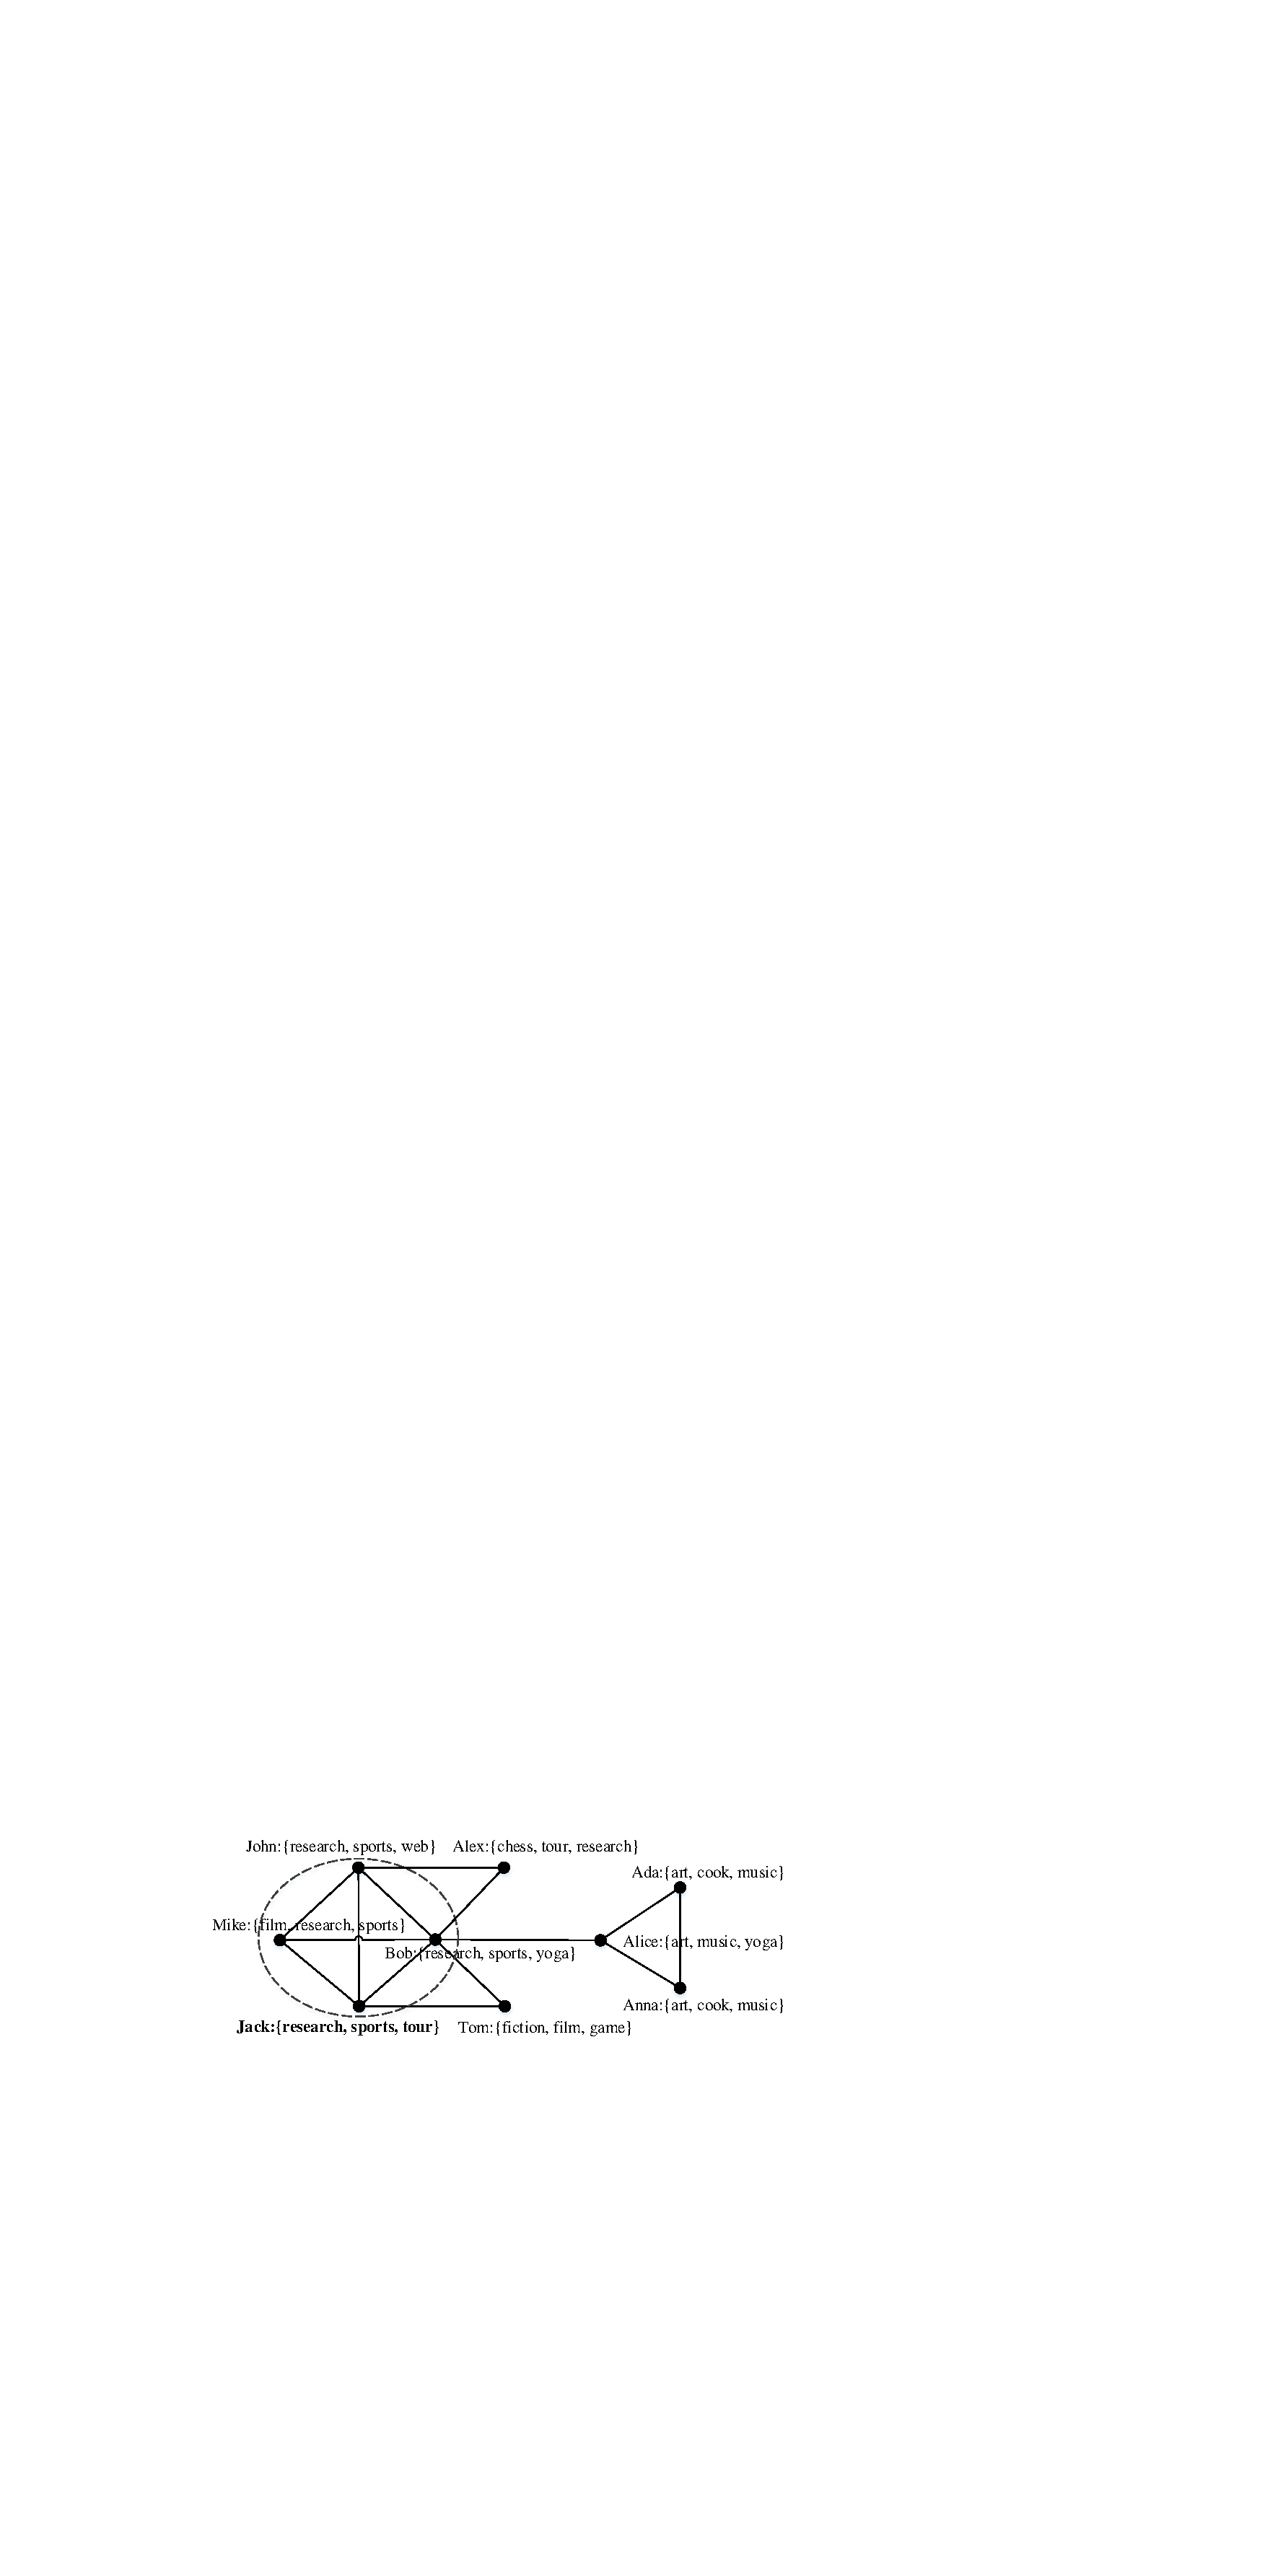
\includegraphics[width=0.88\linewidth]{figures/motivation}
	\caption{Attributed graph and AC (circled).}
	\label{fig:motivation}
\end{figure}

In this paper, we investigate the {\it attributed community query} (or ACQ). Given an attributed graph $G$ and a vertex $q \in G$, the ACQ returns one or more subgraphs of $G$ known as {\it attributed communities} (or ACs).  An AC is a kind of {\it community}, which consists of vertices that are closely related~\cite{KDD2010,local2014,online-sigmod2013,k-truss2014,community-phy2004,community-phy2010}.  Particularly, an AC satisfies {\it structure cohesiveness} (i.e., its vertices are closely linked to each other) and {\it keyword cohesiveness} (i.e., its vertices have keywords in common). Figure~\ref{fig:motivation} illustrates an AC (circled), which is a connected subgraph with vertex degree 3; its vertices $\{${\tt Jack}, {\tt Bob}, {\tt John}, {\tt Mike}$\}$ have two keywords (i.e., ``research'' and ``sports'') in common.

{\bf Prior works.} %An AC is a kind of {\it community}.
The problems related to retrieving communities from a graph can generally be classified into {\it community detection} (CD) and {\it community search} (CS).  In general, CD algorithms aim to retrieve all communities for a graph~\cite{community-phy2004,community-phy2010,attr-vldb2009,attr-topic-kdd2008,attr-topic-icml2009,attr-topic-sigmod2012,attr-www2013,yang2013community}. These solutions are not ``query-based'', i.e., they are not customized for a query request (e.g., a user-specified query vertex).
%For example, it is not clear how these algorithms can return a community that contain a given vertex $q$.
Moreover, they can take a long time to find all the communities for a large graph, and so they are not suitable for quick or {\it online} retrieval of communities. To solve these problems, CS solutions have been recently developed~\cite{KDD2010,local2014,online-sigmod2013,k-truss2014,huang2015approximate,barbieri2015efficient}. These approaches are query-based, and are able to derive communities in an ``online'' manner. However, existing CS algorithms assume {\it non-attributed} graphs, and only use the graph structure information to find communities. The ACQ is a class of CS problem for attributed graphs. As we will show, the use of keyword information can significantly improve the effectiveness of the communities retrieved. Table~\ref{tab:method} summarizes some representative existing works in this area.

\begin{table}
  \centering \footnotesize \caption {Classification of works in community retrieval. }\label{tab:method}
  \begin{tabular}{c|c|c}
     \hline
        \tabincell{c}{\textbf{Graph}\\ \textbf{Type}}
                       & \tabincell{c}{\textbf{Community}\\ \textbf{detection (CD)}}
                       & \tabincell{c}{\textbf{Community}\\ \textbf{search (CS)}}\\
     \hline\hline
        Non-attributed & \cite{community-phy2004,community-phy2010}
                       & \cite{KDD2010,local2014,online-sigmod2013,k-truss2014,vldb2015,huang2015approximate}\\
     \hline
        Attributed     & \cite{attr-vldb2009,attr-topic-kdd2008,attr-topic-icml2009,attr-topic-sigmod2012,attr-www2013,yang2013community}
                       & {\bf ACQ}\\
     \hline
  \end{tabular}
\end{table}

{\bf Features of ACs.} We now present more details about ACs.

\noindent $\bullet$ {\bf Ease of interpretation.}
As demonstrated in Figure~\ref{fig:motivation}, an AC contains tightly-connected vertices with similar contexts or backgrounds. Thus, an ACQ user can focus on the common keywords or features of these vertices (e.g., the vertices of the AC in this example contain ``research'' and ``sports'', reflecting that all members of this AC like research and sports).  We call the set of common keywords among AC vertices
the \emph{AC-label}. In our experiments, the AC-labels facilitate understanding of the vertices that form the AC.

The design of ACs allows it to be used in setting up of social events. For example, if a Twitter member has many keywords about traveling (e.g., he posted a lot of photos about his trips, with keywords), issuing an ACQ with this member as the query vertex may return other members interested in traveling,  because their vertices also have keywords related to traveling. A group tour can then be recommended to these members.

\noindent $\bullet$ {\bf Personalization.}  The user of an ACQ can control the semantics of the AC, by specifying a set of $S$ of keywords. Intuitively, $S$ decides the meaning of the AC based on the user's need.  If we let $q$={\tt Jack}, $k$=2 and $S$=$\{$``research''$\}$,  the AC is formed by
$\{${\tt Jack}, {\tt Bob}, {\tt John}, {\tt Mike}, {\tt Alex}$\}$, who are all interested in research.
Let us consider another example in the DBLP bibliographical network, where each vertex's attribute is represented by the top-20 frequent keywords in their publications. Let $q$={\tt Jim} {\tt Gray}. If $S$ is the set of keywords \{transaction, data, management, system, research\}, we obtain the AC in Figure~\ref{fig:jim}(a), which contains six prominent database researchers closely related to Jim. On the other hand, when $S$ is \{sloan, digital, sky, survey, SDSS\}, the ACQ yields another AC in Figure~\ref{fig:jim}(b), which indicates the seven scientists involved in the SDSS project~\footnote{URL of the SDSS project: \url{http://www.sdss.org}.}.  Thus, with the use of different keyword sets $S$, different ``personalized'' communities can be obtained.

Existing CS algorithms, which do not handle attributed graphs, may not produce the two ACs above. For example, the CS algorithm in \cite{KDD2010} returns the community with {\it all} the 14 vertices shown in Figures~\ref{fig:jim}(a) and (b). The main reasons are: (1) these vertices are heavily linked with Jim; and (2) the keywords are not considered. In contrast, the use of set $S$ in the ACQ places these vertices into two communities, containing vertices that are cohesive in terms of {\it structure} and {\it keyword}. This allows a user to focus on the important vertices that are related to $S$. For example, using the AC of Figure~\ref{fig:jim}(a), a database conference organizer can invite speakers who have a close relationship with Jim.

The personalization feature is also useful in marketing. Suppose that Mary, a yoga lover, is a customer of a gym. An ACQ can be issued on a social network, with Mary as the query vertex and $S$=$\{$``yoga''$\}$. Since members of the AC contain the keyword ``yoga'', they can be the gym's advertising targets. On the other hand, current CS algorithms may return a community that contains one or more vertices without the keyword ``yoga''. It is not clear whether the corresponding user of this vertex is interested in yoga.

\noindent $\bullet$ {\bf Online evaluation.}  Similar to other CS solutions, we have developed efficient ACQ algorithms for large graphs, allowing ACs to be generated quickly upon a query request. On the contrary, existing CD algorithms~\cite{attr-vldb2009,attr-www2013,attr-topic-kdd2008,attr-topic-icml2009} that generate all communities for a graph are often considered to be offline solutions, since they are often costly and time-consuming, especially on very large graphs.

{\bf Technical challenges and our contributions.}
We face two important questions: (1) What should be a sound definition of an AC? (2) How to evaluate ACQ efficiently?  For the first question, we define an AC based on the {\it minimum degree}, which is one of the most common structure cohesiveness metrics~\cite{community-phy2004,community-phy2010,KDD2010,local2014}. This measure requires that every vertex in the community has a degree of $k$ or more.
%one of the most fundamental characteristics of graphs, and some recent works~\cite{KDD2010,local2014} have shown that it is better than many other metrics like average degree and density of a graph.
We formulate the keyword cohesiveness as maximizing the number of shared keywords in keyword set $S$. The shared keywords naturally reveal the common features among vertices (e.g., common interest of social network users). We can also use these shared keywords to explain how a community is formed.

\begin{figure}[ht]
    \centering
    \mbox{
        \subfigure[$S$=\{transaction, data, management, system, research\}]{
            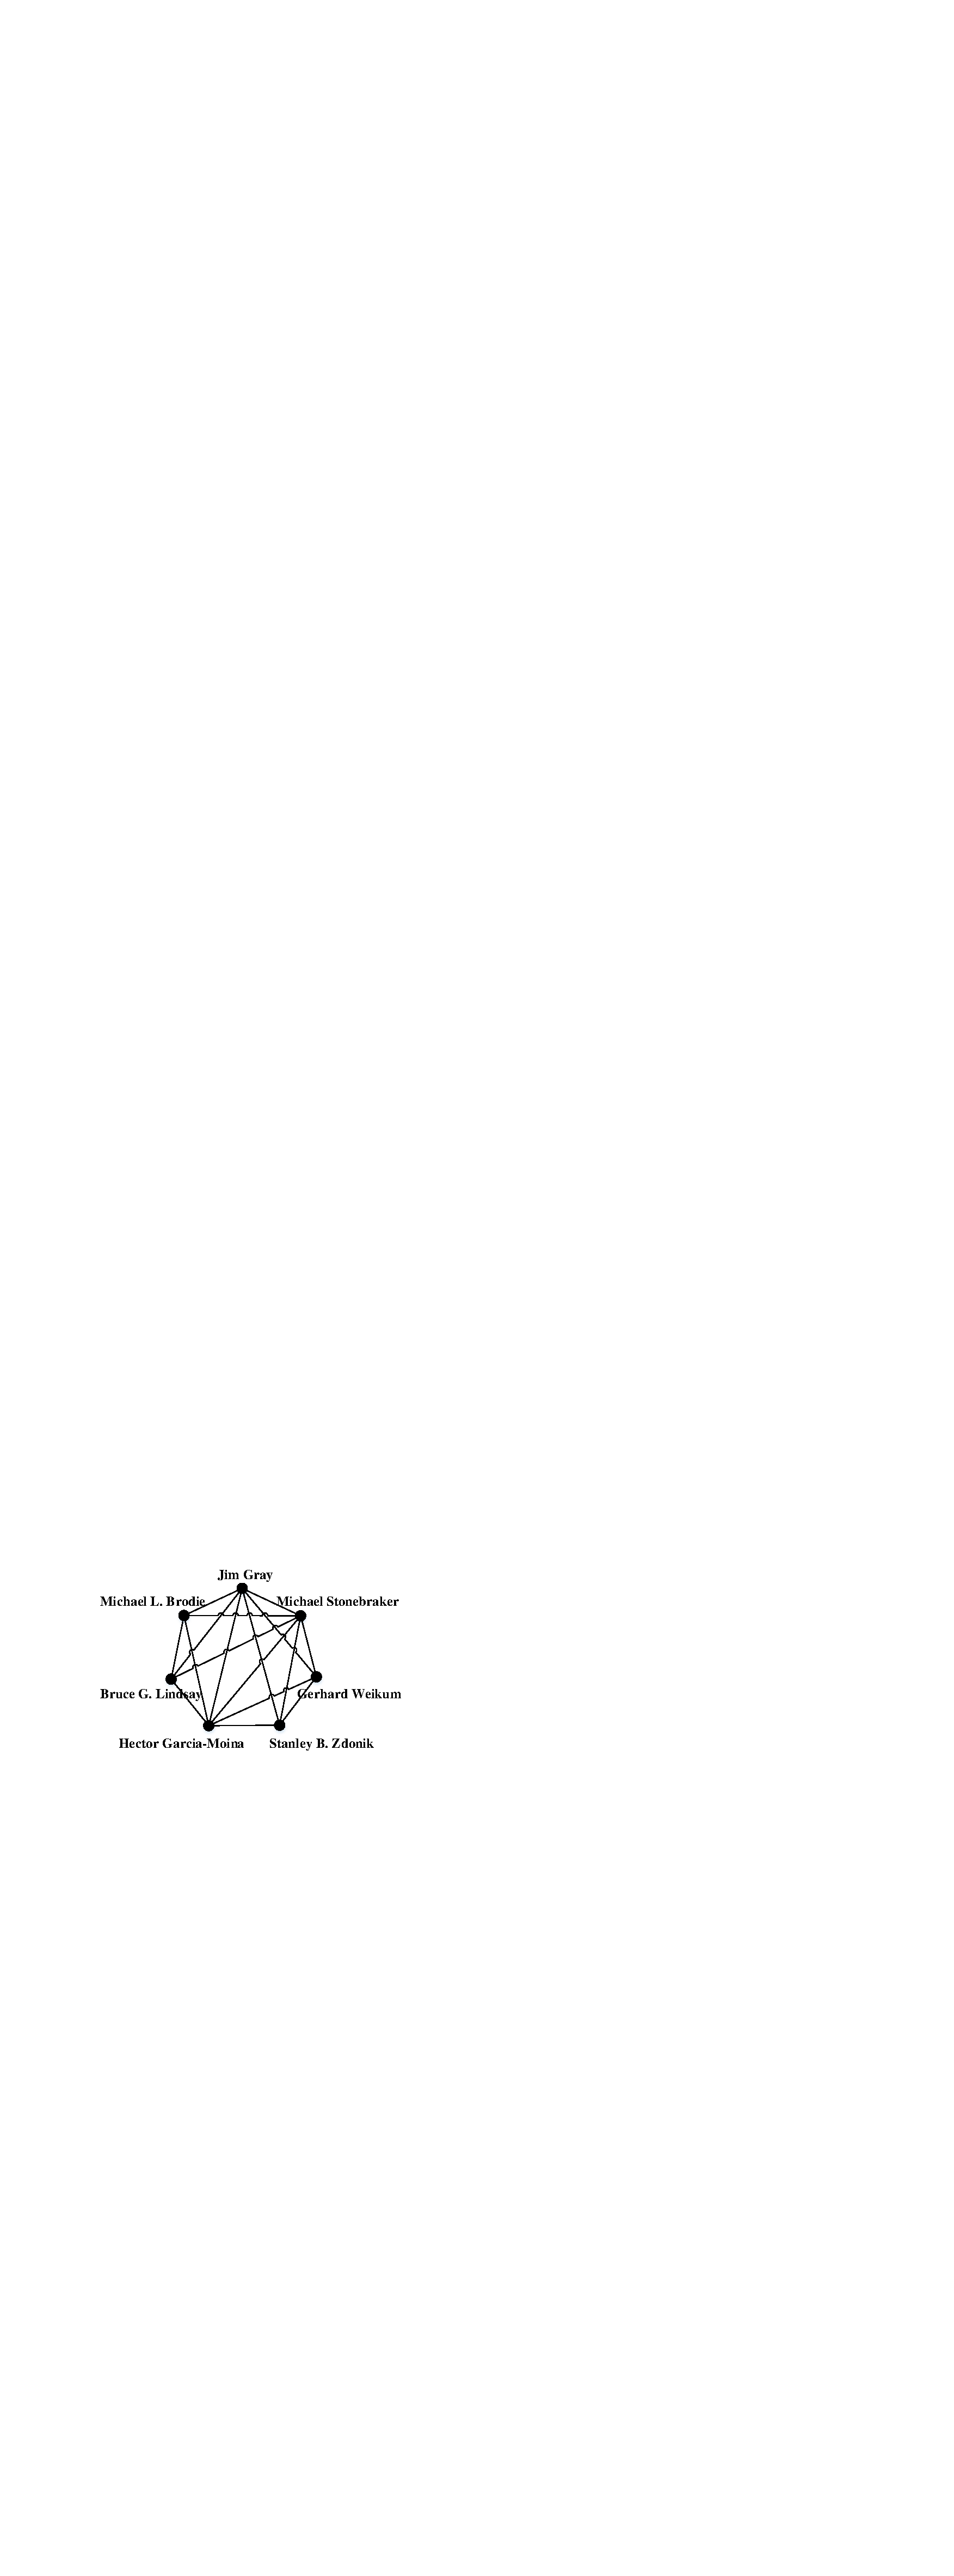
\includegraphics[width=.44\columnwidth]{figures/jim1}
            \label{fig:jim1}
        }
        \hspace{1ex}
        \subfigure[$S$=\{sloan, digital, sky, data, sdss\}]{
            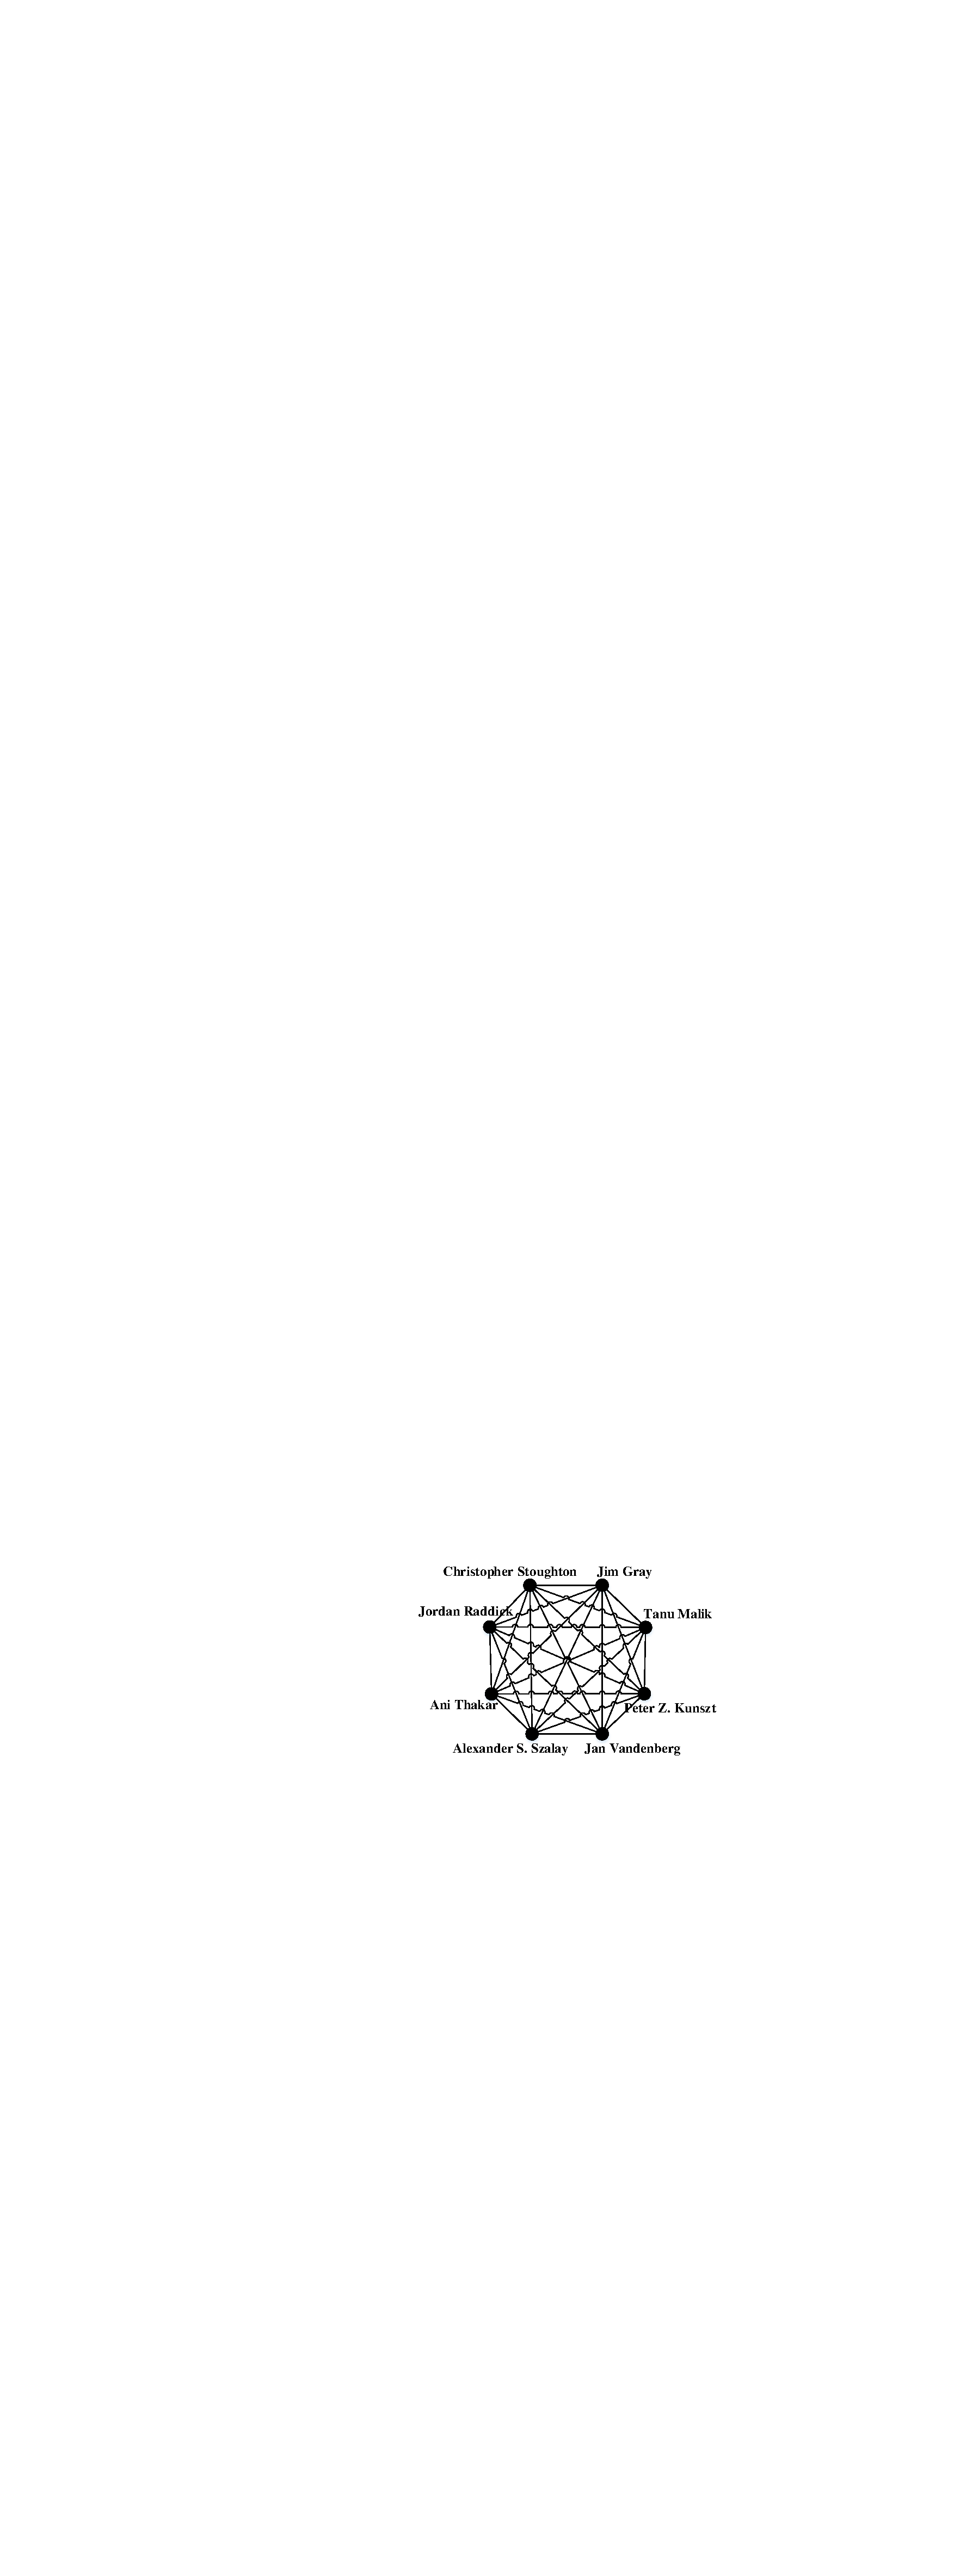
\includegraphics[width=.432\columnwidth]{figures/jim2}
            \label{fig:jim2}
        }
    }
    \caption{Two ACs of Jim Gray.}\label{fig:jim}
\end{figure}

The second question is not easy to answer, because the attributed graph $G$ to be explored can be very large, and the (structure and keyword) cohesiveness criteria can be complex to handle. A simple way is first to consider all the possible keyword combinations, and then return the subgraphs, which satisfy the minimum degree constraint and have the most shared keywords. This solution, which requires the enumeration of all the subsets of $q$'s keyword set, has a complexity exponential to the size $l$ of $q$'s keyword set. In our experiments, for some queries, $l$ can be up to 30, resulting in the consideration of $2^{30}=1,073,741,824$ subsets of $q$. The algorithm is impractical, especially when $q$'s keyword set is large.

{\color{blue}
We observe the {\it anti-monotonicity} property, which states that given a set $S$ of keywords, if it appears in every vertex of an AC, then for every subset $S'$ of $S$, there exists an AC in which every vertex contains $S'$. We use this intuition to propose better algorithms. We further develop the \emph{CL-tree}, an index that organizes the vertex keyword data in a hierarchical structure. The CL-tree has a space and construction time complexity linear to the size of $G$.
Based on the CL-tree index, we have developed three different ACQ algorithms based on the CL-tree, and they are able to achieve a superior performance.
Moreover, to maintain the CL-tree index for dynamic graphs in which the keywords and edges are inserted or deleted, we have develop efficient algorithms for maintaining the CL-tree without re-building it from scratch.

In addition, we have proposed two typical variants of the ACQ problems. The first one is an approximation version of the ACQ query in which vertices of an AC do not need to exactly share the same keywords in $S$;
the second one considers multiple query vertices and outputs their ACs.
To answer the queries for these variants, we have also developed efficient algorithms based on the CL-tree index.
}

We have performed extensive experiments on four large real graph datasets (namely Flickr, DBLP, Tencent, and DBpedia).
We found that a large number of common keywords appear across vertices in our graph datasets. In DBLP, for instance, an AC with one common keyword contains over 5,000 vertices on average; an AC with two common keywords contains over 700 vertices. Hence, using shared keywords among vertices as keyword cohesiveness makes sense.
We have also studied how to quantify the quality of a community, based on occurrence frequencies of keywords and similarity between the keyword sets of two vertices. We conducted a detailed case study on DBLP. These results confirm the superiority of the AC over the communities returned by existing community detection and community search algorithms, in terms of community quality. The performance of our best algorithm is 2 to 3 order-of-magnitude better than solutions that do not use the CL-tree. Another advantage of our approaches is that they organize and search vertex keywords for ACs effectively, achieving a higher efficiency than existing community search solutions (that do not use vertex keywords in the community search process).

{\bf Organization.} We review the related work in Section~\ref{related}, and define the ACQ problem formally in Section~\ref{problem}. Section~\ref{basic} presents the basic solutions, and Section~\ref{index} discusses the CL-tree index.
In Section~\ref{indexMaintenance}, we discuss how to maintain the CL-tree index for dynamic graphs.
We present the query algorithms in Section~\ref{query}.
In Section~\ref{variant}, we introduce two variants and the corresponding query algorithms.
Our experimental results are reported in Section~\ref{experiment}.
We conclude in Section~\ref{conclusion}. 

\section{Related Work}
\label{related}

%We now discuss two main classes of community retrieval solutions. We also summarize the graph keyword search solutions for attributed graphs.

\textbf{Community detection (CD).} A large class of studies aim to discover or {\it detect} all the communities from an entire graph. Table~\ref{tab:method} summarises these works. Earlier solutions, such as \cite{community-phy2004,community-phy2010}, employ link-based analysis to obtain these communities. However, they do not consider the textual information associated with graphs. Recent works focus on attributed graphs, and use clustering techniques to identify communities.
%Clustering is a typical way to discover communities.
For instance, Zhou et al.~\cite{attr-vldb2009} considered both links and keywords of vertices to compute the vertices' pairwise similarities, and then clustered the graph.
Ruan et al.~\cite{attr-www2013} proposed a method called {\tt CODICIL}. This solution augments the original graphs by creating new edges based on content similarity, and then uses an effective graph sampling to boost the efficiency of clustering. We will compare ACQ with this method experimentally.

Another common approach is based on topic models. In~\cite{attr-topic-kdd2008,attr-topic-icml2009}, the {\tt Link-PLSA-LDA} and {\tt Topic-Link LDA} models jointly model vertices' content and links based on the {\tt LDA} model. In~\cite{attr-topic-sigmod2012}, the attributed graph is clustered based on probabilistic inference. In~\cite{attr-topic-www2012}, the topics, interaction types and the social connections are considered for discovering communities. {\tt CESNA}~\cite{attr-icdm2013} detects overlapping communities by assuming communities ``generate'' both the link and content. A discriminative approach~\cite{attr-kdd2009} has also been considered for community detection. As discussed before, CD algorithms are generally slow, as they often consider the pairwise distance/similarity among vertices.
Also, it is not clear how they can be adapted to perform online ACQ. In this paper, we propose online algorithms for finding communities on attributed graphs.

\textbf{Community search (CS).}  Another class of solutions aims to obtain communities in an ``online'' manner, based on a query request. For example, given a vertex $q$, several existing works~\cite{KDD2010,local2014,vldb2015,online-sigmod2013,k-truss2014} have developed fast algorithms to obtain a community for $q$.
To measure the structure cohesiveness of a community, the {\it minimum degree} is often used~\cite{KDD2010,local2014,vldb2015}. Sozio et al.~\cite{KDD2010} proposed the first algorithm {\tt Global} to find the $k$-$\widehat{core}$ containing $q$.
Cui et al.~\cite{local2014} proposed {\tt Local}, which uses local expansion techniques to enhance the performance of {\tt Global}. We will compare these two solutions in our experiments.
Other definitions, including $k$-clique~\cite{online-sigmod2013}, $k$-truss~\cite{k-truss2014} and edge connectivity~\cite{hu2016querying}, have also been considered for searching communities. A recent work~\cite{vldb2015} finds communities with high influence.  These works assume non-attributed graphs, and overlook the rich information of vertices that come with attributed graphs. As we will see, performing CS on attributed graphs is better than on non-attributed graphs.

\textbf{Graph keyword search.}  Given an attributed graph $G$ and a set $Q$ of keywords, graph keyword search solutions output a tree structure, whose nodes are vertices of $G$, and the union of these vertices' keyword sets is a superset of $Q$~\cite{keyword-icde2002,keyword-icde2007,keyword-vldb2005}. Recent work studies the use of a subgraph of $G$ as the query output~\cite{keyword-vldb2011}. These works are substantially different from the ACQ problem. First, they do not specify query vertices as required by the ACQ problem. Second, the tree or subgraph produced do not guarantee structure cohesiveness. Third, keyword cohesiveness is not ensured; there is no mechanism that enforces query keywords to be shared among the keyword sets of all query output's vertices. Thus, these solutions are not designed to find ACs.

%{\color{red}
%\textbf{Graph pattern matching (GPM).}  Given a {\it pattern} $P$, the goal of GPM is to extract a set $R$ of subgraphs of $G$, where for every $r \in R$, $r$ is highly similar to $P$.
%Tong et al.~\cite{GPM-KDD2007} studied the use of lines, loops and stars; Fan et al.~\cite{GPM-VLDB2010,GPM-SIGMOD2011} proposed bounded simulation techniques for GPM queries;
%in \cite{GPM-PVLDB2015}, GPM has been studied for finding association rules from graphs.
%However, there is no detailed study about how to use GPM for community search.
%}

%Older version: July 12, 2016
%\textbf{Graph pattern matching (GPM).}  Given a {\it pattern} $P$, the goal of GPM is to extract a set $R$ of subgraphs of $G$, where for every $r \in R$, $r$ is highly similar to $P$.
%Tong et al.~\cite{GPM-KDD2007} studied the use of lines, loops and stars; Fan et al.~\cite{GPM-VLDB2010,GPM-SIGMOD2011} proposed bounded simulation techniques for GPM queries;
%in \cite{GPM-PVLDB2015}, GPM has been studied for finding association rules from graphs.
%However, there is no detailed study about how to use GPM for community search.  To do this, a user has to define $P$, but this is not trivial: there are many possible topologies for $P$, and numerous ways of placing keywords on the vertices in $P$.  Moreover, current GPM solutions focus on small patterns that generate small communities, and it is not clear whether they can support large and complex ones. Answering ACQ with GPM can also be expensive, since it involves enumerating many patterns and finding an AC with the largest number of shared keywords.  For the ACQ problem, there is no need to specify $P$.


\section{The ACQ Problem}
\label{problem}

We now discuss the attributed graph model, the $k$-core, and the AC.  In the CS and CD literature, most existing works assume that the underlying graph is undirected~\cite{KDD2010,vldb2015,attr-topic-sigmod2012,attr-www2013}.
We also suppose that an attributed graph $G(V,E)$ is undirected, with vertex set $V$ and edge set $E$. Each vertex $v \in V$ is associated with a set of keywords, $W(v)$. Let $n$ and $m$ be the corresponding sizes of $V$ and $E$. The degree of a vertex $v$ of $G$ is denoted by $deg_G(v)$. Table~\ref{tab:notation} lists the symbols used in the paper.

\begin{table}[]
  \centering \footnotesize \caption {Symbols and meanings.}
  \label{tab:notation}
  \small
  \begin{tabular}{c|l}
     \hline
          {\bf Symbol} & {\bf Meaning}\\
     \hline\hline
          $G(V,E)$       & An attributed graph with vertex set $V$ and edge set $E$\\ %($n$=$|V|$, $m$=$E$)
     \hline
          $W(v)$         & The keyword set of vertex $v$\\
     \hline
          $deg_G(v)$     & The degree of vertex $v$ in $G$\\
     \hline
          $G[S']$        & \tabincell{l}{The largest connected subgraph of $G$ s.t. $q\in G[S']$,\\
                           and $\forall v\in G[S']$, $S'\subseteq W(v)$}\\
     \hline
          $G_k[S']$      & \tabincell{l}{The largest connected subgraph of $G$ s.t. $q\in G_k[S']$,\\
                           and $\forall v\in G_k[S']$, $deg_{G_k[S']}v\geq k$ and $S'\subseteq W(v)$}\\
     \hline
  \end{tabular}
\end{table}

A community is often a subgraph of $G$ that satisfies {\it structure cohesiveness} (i.e., the vertices contained in the community are linked to each other in some way). A common notion of structure cohesiveness is that
the \emph{minimum degree} of all the vertices that appear in the community has to be $k$ or more~\cite{KDD2010,md1983,kcore2003,kcore2006,local2014,vldb2015}.
This is used in the $k$-core and the AC. Let us discuss the $k$-core first.

\begin{definition}[$k$-core~\cite{md1983,kcore2003}]
\label{def:kcore}
Given an integer $k$ ($k\geq 0$), the $k$-core of $G$,
denoted by $H_{k}$, is the largest subgraph of $G$, such that $\forall v \in H_k$, $deg_{H_k}(v) \geq k$.
\end{definition}

We say that $H_k$ has an order of $k$.  Notice that $H_k$ may not be a connected graph~\cite{kcore2003}, and its connected components, denoted by $k$-$\widehat{core}$s, are usually the ``communities'' returned by $k$-$\widehat{core}$ search algorithms.

\begin{figure}[ht]
    \centering
    \mbox{
        \subfigure[graph]{
            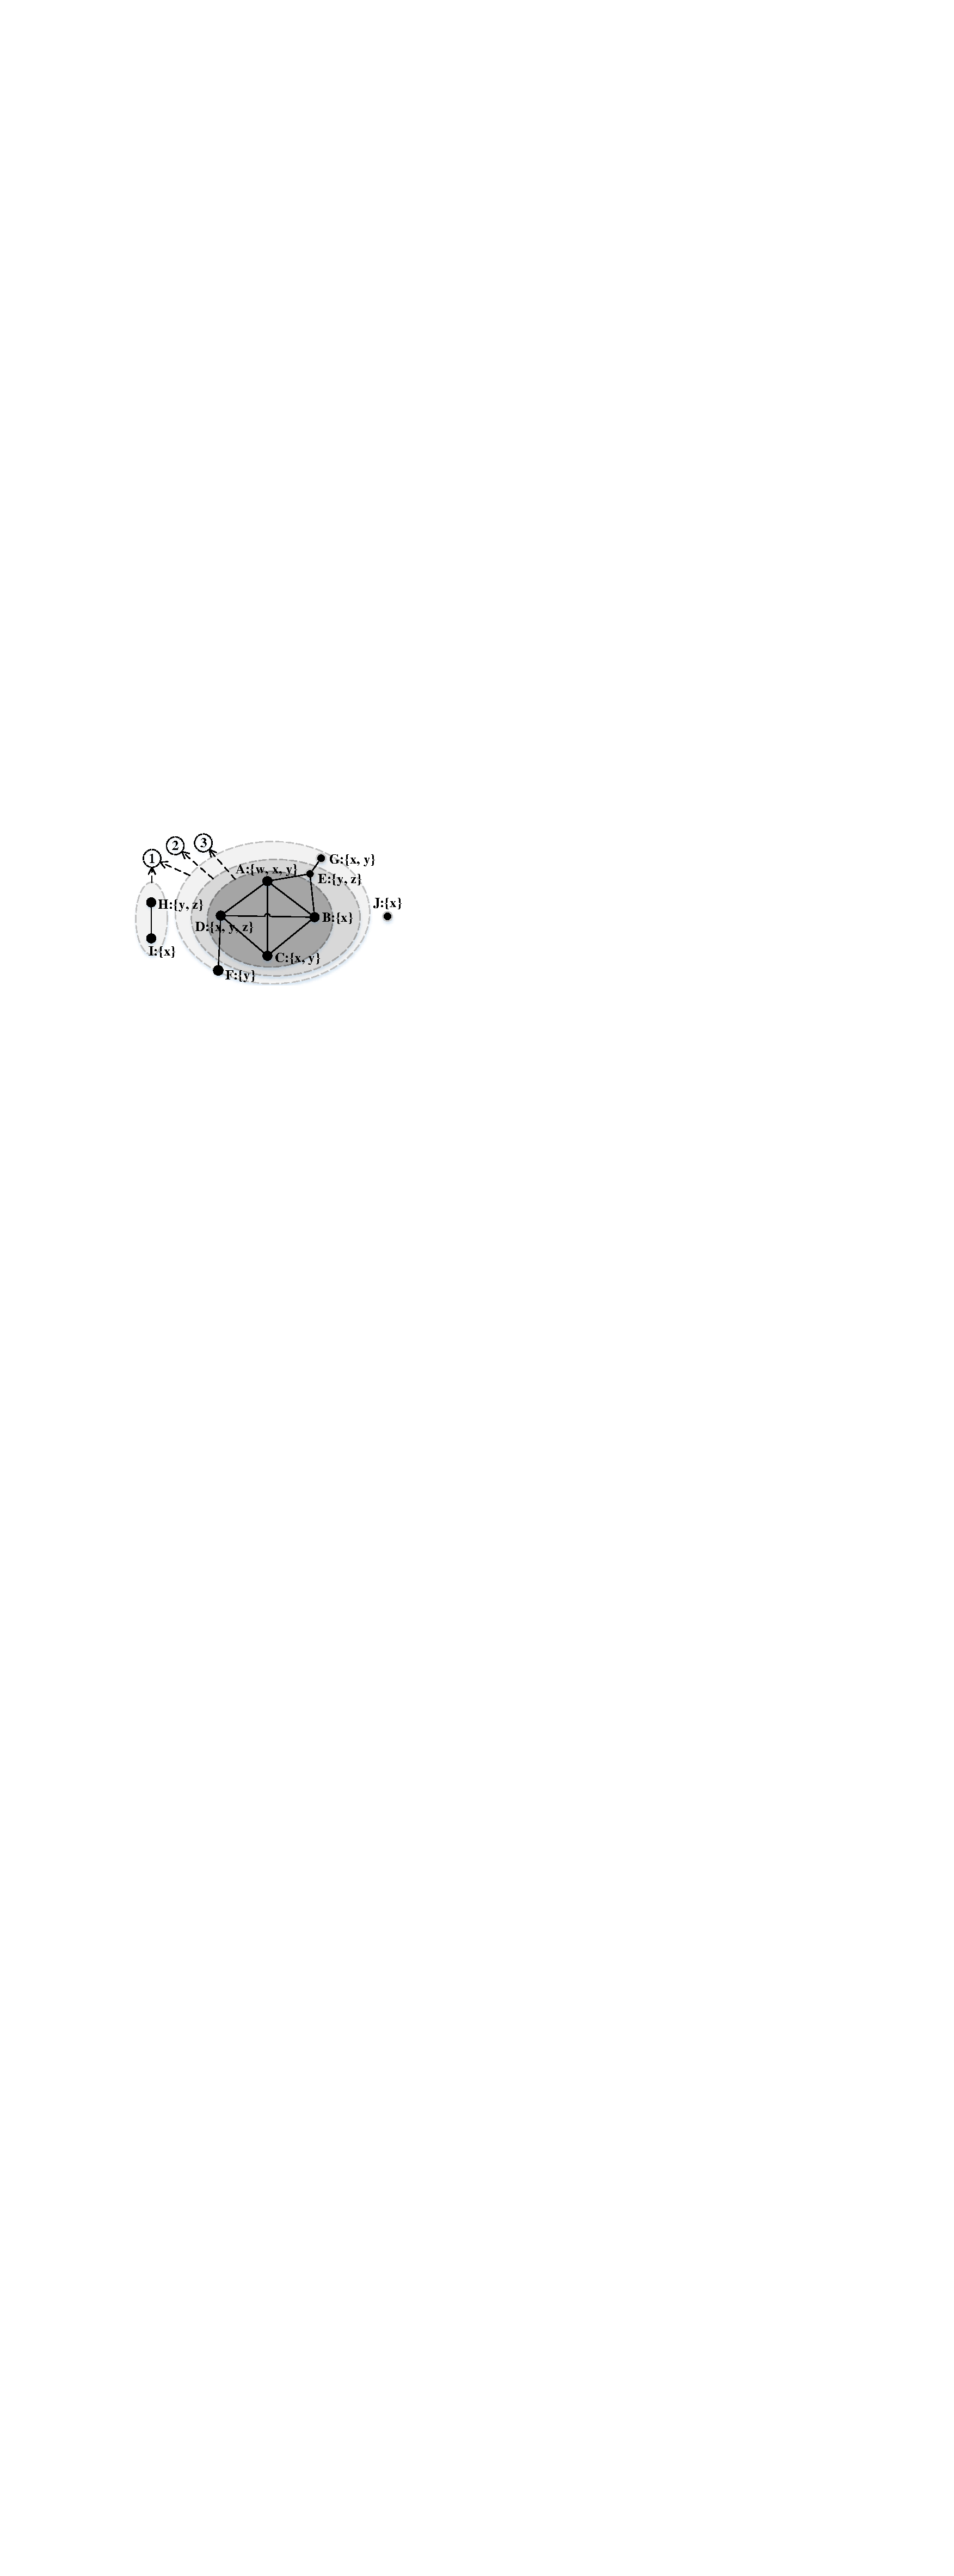
\includegraphics[width=.46\columnwidth]{figures/kcoreGraph}
            \label{fig:kcoreGraph}
        }
        \hspace{1ex}
        \subfigure[core number]{
            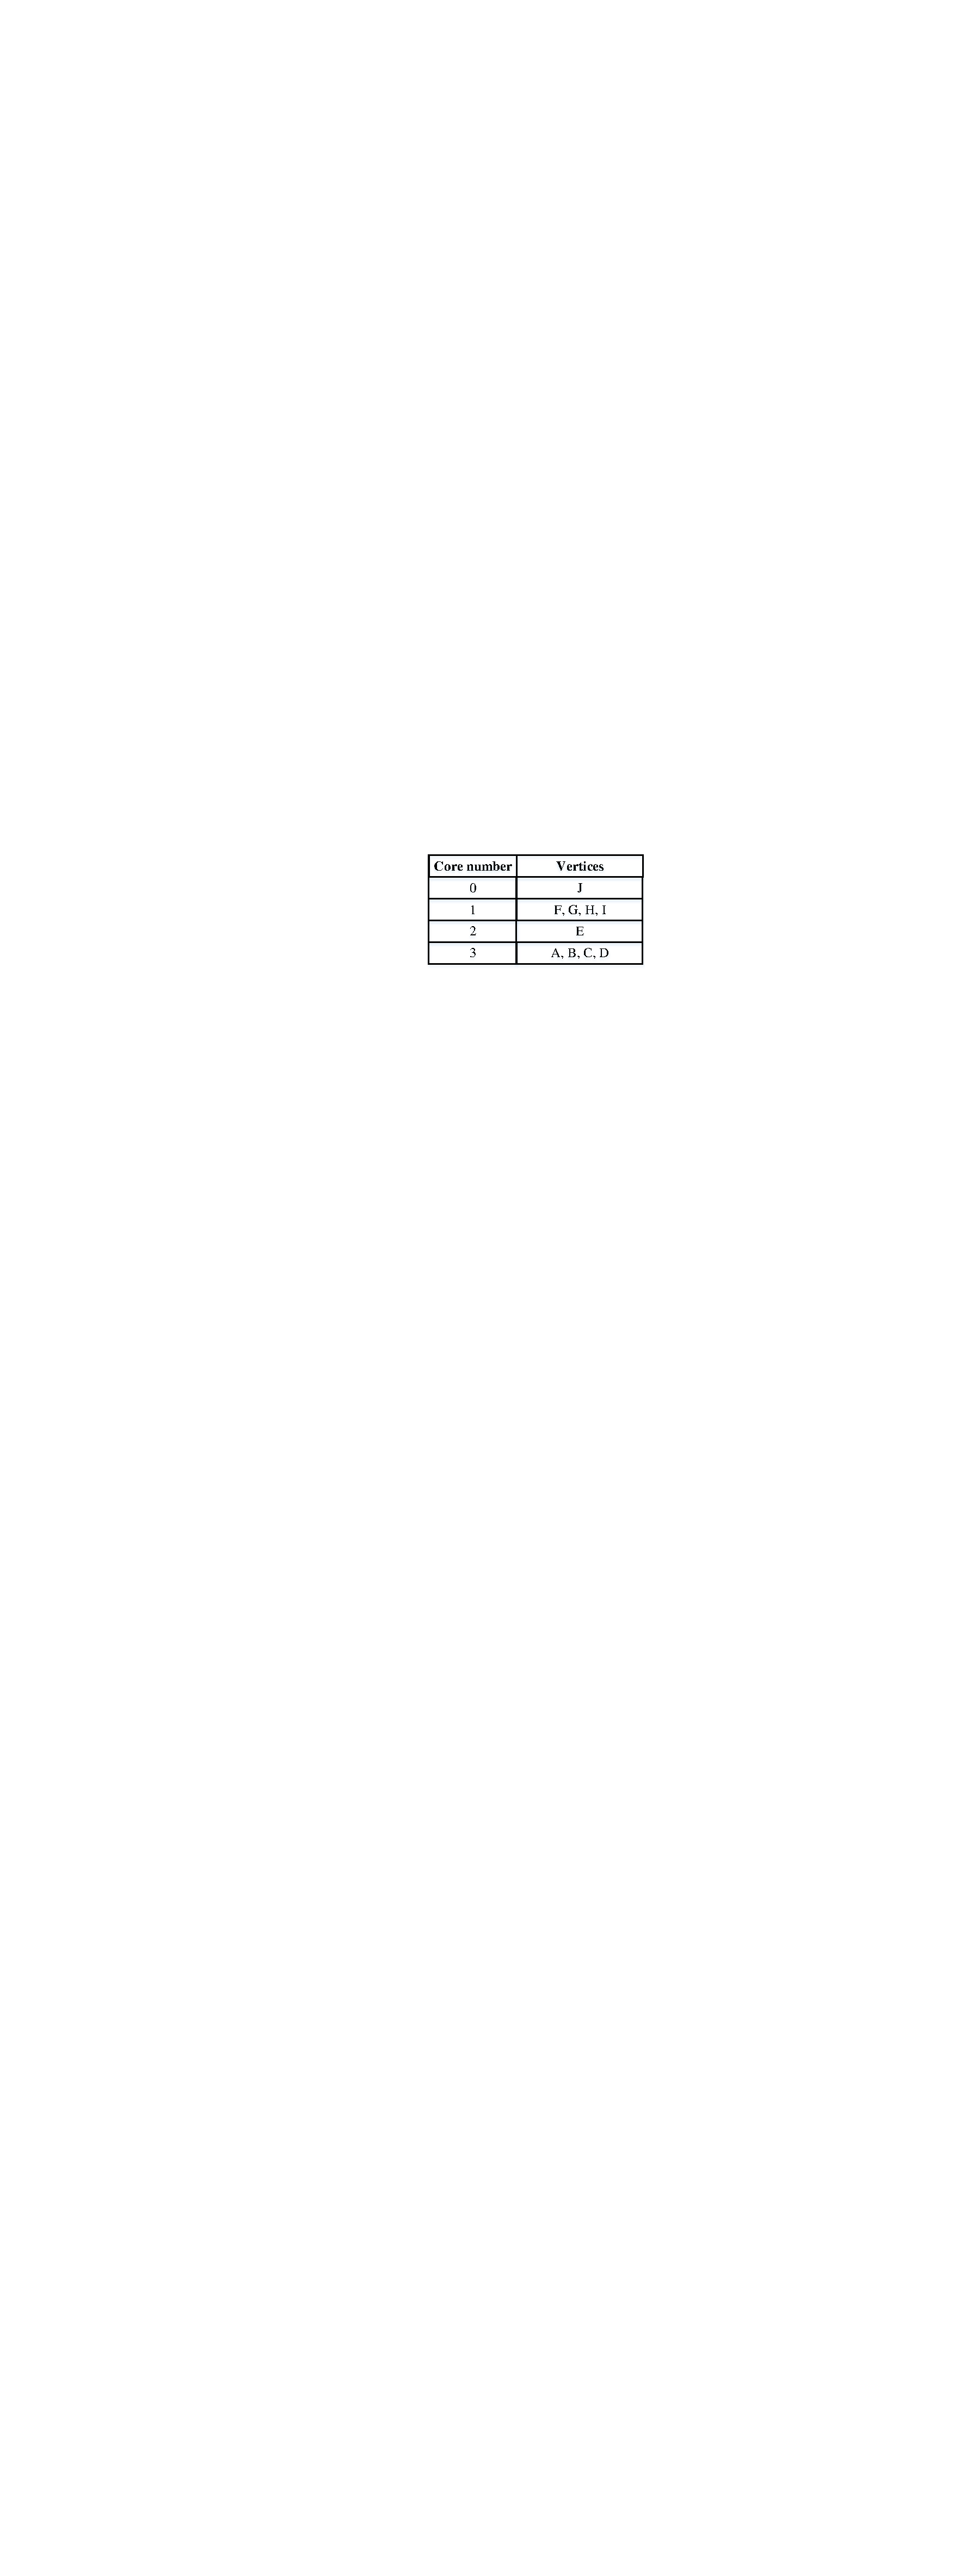
\includegraphics[width=.40\columnwidth]{figures/kcoreTable}
            \label{fig:kcoreTable}
        }
    }
    \caption{Illustrating the $k$-core and the AC.}
\end{figure}

\begin{example}
\label{eg:problem}
In Figure~\ref{fig:kcoreGraph}, $\{A,B,C,D\}$ is both a 3-core and a 3-$\widehat{core}$. The 1-core has vertices $\{A,B,C,D,E,F,G,$ $H,I\}$, and is composed of two $1$-$\widehat{core}$ components: $\{A,B,$ $C,D,E,F,G\}$ and $\{H,I\}$. The number $k$ in each circle represents the $k$-$\widehat{core}$ contained in that ellipse.
\end{example}

Observe that $k$-$core$s are ``nested''~\cite{kcore2003}: given two positive integers $i$ and $j$, if $i<j$, then $H_j \subseteq H_i$.  In Figure~\ref{fig:kcoreGraph}, $H_3$ is contained in $H_2$, which is nested in $H_1$.

\begin{definition}[Core number]
\label{def:coreNum}
Given a vertex $v \in V$, its core number, denoted by $core_G[v]$, is the highest order of a $k$-core that contains $v$.
\end{definition}

A list of core numbers and their respective vertices for Example~\ref{eg:problem} are shown in Figure~\ref{fig:kcoreTable}. In~\cite{kcore2003}, an $O(m)$ algorithm was proposed to compute the core number of every vertex.

%An efficient solution (called {\tt Global}) for finding a $k$-$\widehat{core}$ that contains a vertex $q \in V$ was presented in \cite{KDD2010}. Recently, Cui et al. have developed a fast solution called {\tt Local}~\cite{local2014}, yielding subgraph(s) of $k$-$\widehat{core}$ that satisfy structure cohesiveness. In Section~\ref{experiment}, we compare our approach with {\tt Global} and {\tt Local}.

%As discussed in Section~\ref{intro}, two vertices that do not share any keywords may still be placed together in a $k$-$\widehat{core}$. In Example~\ref{eg:problem}, $H$ and $I$ are included in the $1$-$\widehat{core}$ even though their keywords are completely different. To address this issue, we introduce the LAC search problem.

We now formally define the ACQ problem as follows.

\begin{problem}[ACQ]
\label{problem1}
Given a graph $G(V,E)$, a positive integer $k$, a vertex $q \in V$ and a set of keywords $S\subseteq W(q)$, return a set $\mathcal {G}$ of graphs, such that $\forall G_q \in \mathcal {G}$, the following properties hold:


\vspace{1ex}
$\bullet$ \textbf{Connectivity}. $G_q \subseteq G$ is connected and $q\in G_q$;

$\bullet$ \textbf{Structure cohesiveness}. $\forall$$v\in G_q$, $deg_{G_q}(v)\geq$$k$;

$\bullet$ \textbf{Keyword cohesiveness}. The size of $L(G_q, S)$ is maximal, where $L(G_q, S)=\cap_{v \in G_q}(W(v)\cap S)$ is the set of keywords shared in $S$ by all vertices of $G_q$.%\vspace{1ex}
\end{problem}

We call $G_q$ the {\it attributed community} (or AC) of $q$, and $L(G_q, S)$ the {\it AC-label} of $G_q$. In Problem~\ref{problem1}, the first two properties are also specified by the $k$-$\widehat{core}$ of a given vertex $q$~\cite{KDD2010}. The {\it keyword cohesiveness} (Property 3), which is unique to Problem~\ref{problem1}, enables the retrieval of communities whose vertices have common keywords in $S$.  We use
$S$ to impose semantics on the AC produced by Problem~\ref{problem1}. By default, $S=W(q)$, which means that the AC generated should have keywords common to those associated with $q$. If $S \subset W(q)$, it means that the ACQ user is interested in forming communities that are related to some (but not all) of the keywords of $q$. A user interface could be developed to display $W(q)$ to the user, allowing her to include the desired keywords into $S$.  For example, in Figure~\ref{fig:kcoreGraph}, if $q$=$A$, $k$=2 and $S$=$\{w,x,y\}$, the output of Problem~\ref{problem1} is $\{A,C,D\}$, with AC-label $\{x,y\}$, meaning that these vertices share the keywords $x$ and $y$.


We require $L(G_q, S)$ to be maximal in Property 3, because we wish the AC(s) returned only contain(s) the most related vertices, in terms of the number of common keywords. Let us use Figure~\ref{fig:kcoreGraph} to explain why this is important. Using the same query ($q$=$A$,$k$=2,$S$= $\{w,x,y\}$), without the ``maximal'' requirement, we can obtain communities such as $\{A,B,E\}$ (which do not share any keywords), $\{A,B,D\}$, or $\{A,B,C\}$ (which share 1 keyword). Note that there does not exist an AC with AC-label being exactly $\{w$, $x,y\}$.
Our experiments (Section~\ref{experiment}) show that imposing the ``maximal'' constraint yields the best result. Thus, we adopt Property 3 in Problem~\ref{problem1}.
If there is no AC whose vertices share one or more keywords
(\textit{i.e.}, $|L(G_q, S)|$=0), we return the subgraph of $G$ that satisfies Properties 1 and 2 only.
~\footnote{In practice, the query user can be alerted by the system when there is no sharing among the vertices.}

There are other candidates for structure cohesiveness (e.g., $k$-truss, $k$-clique) and  {\it keyword cohesiveness} (e.g., Jaccard similarity and string edit distance). An AC can also be defined in different ways. For example, an ACQ user may specify that an AC returned must have vertices that contain a specific set of keywords.
An interesting direction is to extend ACQ  to support for these criteria, and study their effectiveness.


\section{Basic Solutions}
\label{basic}

For ease of presentation, we say that $v$ contains a set $S'$ of keywords, if $S'\subseteq W(v)$.
We use $G[S']$ to denote the largest connected subgraph of $G$,
where each vertex contains $S'$ and $q\in G[S]$.
We use $G_k[S']$ to denote the largest connected subgraph of $G[S']$,
in which every vertex has degree being at least $k$ in $G_k[S']$.
We call $S'$ a qualified keyword set for the query vertex $q$ on the graph $G$, if $G_k[S']$ exists.
%We call $G_k[S']$ a target AC, if $S'$ is the largest subset of $S$ and $G_k[S']$ satisfies all the cohesiveness of ACQ problem.

Given a query vertex $q$, a straightforward method to answer ACQ performs three steps.
First, all non-empty subsets of $S$, $S_1,S_2,\cdots$, $S_{2^l-1}$ ($l$=$|S|$), are enumerated.
Then, for each subset $S_i$(1$\leq i\leq2^l-$1), we verify the existence of $G_k[S_i]$ and compute it when it exists (We postpone to discuss the details). Finally, we output the subgraphs having the most shared keywords among all $G_k[S_i]$.

One major drawback of the straightforward method is that we need to compute $2^l-1$ subgraphs (\textit{i.e.}, $G_k[S_i]$).
For large values of $l$, the computation overhead renders the method impractical, and we do not further consider this method in the paper. To alleviate this issue, we propose the following two-step framework.

\subsection{Two-Step Framework}
The two-step framework is mainly based on the following \emph{anti-monotonicity} property.
\begin{lemma}[Anti-monotonicity]
  \label{lemma:apriori}
  Given a graph $G$, a vertex $q\in G$ and a set $S$ of keywords, if there exists a subgraph $G_k[S]$,
  then there exists a subgraph $G_k[S']$ for any subset $S'\subseteq S$.
\end{lemma}

All the proofs of lemmas studied in this paper can be found in Appendix~\ref{app:proof}.
The anti-monotonicity property allows us to stop examining all the super sets of $S' (S'\subseteq S)$, once have verified that $G_k[S']$ does not exist.
The basic solution begins with examining the set, $\Psi_1$, of size-$1$ candidate keyword sets,
\textit{i.e.}, each candidate contains a single keyword of $S$.
It then repeatedly executes the following two key steps,
to retrieve the size-$2$ (size-$3$, \ldots) qualified keyword subsets until no qualified keyword sets are found.

$\bullet$ {\bf Verification.} For each candidate $S'$ in $\Psi_c$ (initially $c$=1),
mark $S'$ as a qualified set if $G_k[S']$ exists.

$\bullet$ {\bf Candidate generation.} For any two current size-$c$ qualified keyword sets which only differ in one keyword, union them as a new expanded candidate with size-($c$+$1$), and put it into set $\Psi_{c+1}$, if all its subsets are qualified, by Lemma~\ref{lemma:apriori}.

Among the above steps, the key issue is how to compute $G_k[S']$.
Since $G_k[S']$ should satisfy the~\emph{structure cohesiveness} (\textit{i.e.}, minimum degree at least $k$)
and~\emph{keyword cohesiveness} (\textit{i.e.}, every vertex contains keyword set $S'$).
Intuitively, we have two approaches to compute $G_k[S']$:
either searching the subgraph satisfying degree constraint first,
followed by further refining with keyword constraints (called {\tt basic-g});
or vise versa (called {\tt basic-w}).
These two algorithms form our baseline solutions.
Their pseudocodes are presented in Appendix~\ref{app:basic}. 

\section{CL-tree Index}
\label{index}
The major limitation of {\tt basic-g} and {\tt basic-w} is that
they need to find the $k$-$\widehat {core}$s and do keyword filtering repeatedly.
This makes the community search very inefficient.
To achieve higher query efficiency, we propose a novel index,
called \textbf{CL-tree} (\underline{C}ore \underline{L}abel tree),
which organizes both the $k$-$\widehat {core}$s and keywords into a tree structure.
Based on the index, the efficiency of answering ACQ and its variants
can be improved significantly.
We first introduce the index in Section~\ref{indexIntro},
and then propose two index construction methods in Section~\ref{indexConstruction}.

\subsection{Index Overview}
\label{indexIntro}
The CL-tree index is built based on the key observation that cores are nested.
Specifically, a $(k$+1$)$-$\widehat {core}$ must be contained in a $k$-$\widehat{core}$.
The rationale behind is, a subgraph has a minimum degree at least $k+1$ implies that
it has a minimum degree at least $k$. Thus, all $k$-$\widehat {core}$s can be organized into a tree structure\footnote{We use ``node'' to mean ``CL-tree node'' in this paper.}. We illustrate this in Example~\ref{eg:index}.

\begin{example}
\label{eg:index}
Consider the graph in Figure~\ref{fig:kcoreGraph}.
All the $k$-$\widehat {core}$s can be organized into a tree as shown in Figure~\ref{fig:ucktree}.
The height of the tree is 4.
For each tree node, we attach the core number and vertex set of its corresponding $k$-$\widehat {core}$.
\end{example}

From the tree structure in Figure~\ref{fig:ucktree}, we conclude that,
if a ($k$+1)-$\widehat {core}$ (denoted as ${\mathcal C}_{k+1}$)
is contained in a $k$-$\widehat {core}$ (denoted as ${\mathcal C}_k$),
then there is a tree node corresponding to ${\mathcal C}_{k+1}$ and its parent node corresponds to ${\mathcal C}_k$.
Besides, the height of the tree is at most $k_{max}+1$, where $k_{max}$ is the maximum core number.

\begin{figure}[ht]
    \centering
    \mbox{
        \subfigure[tree structure]{
            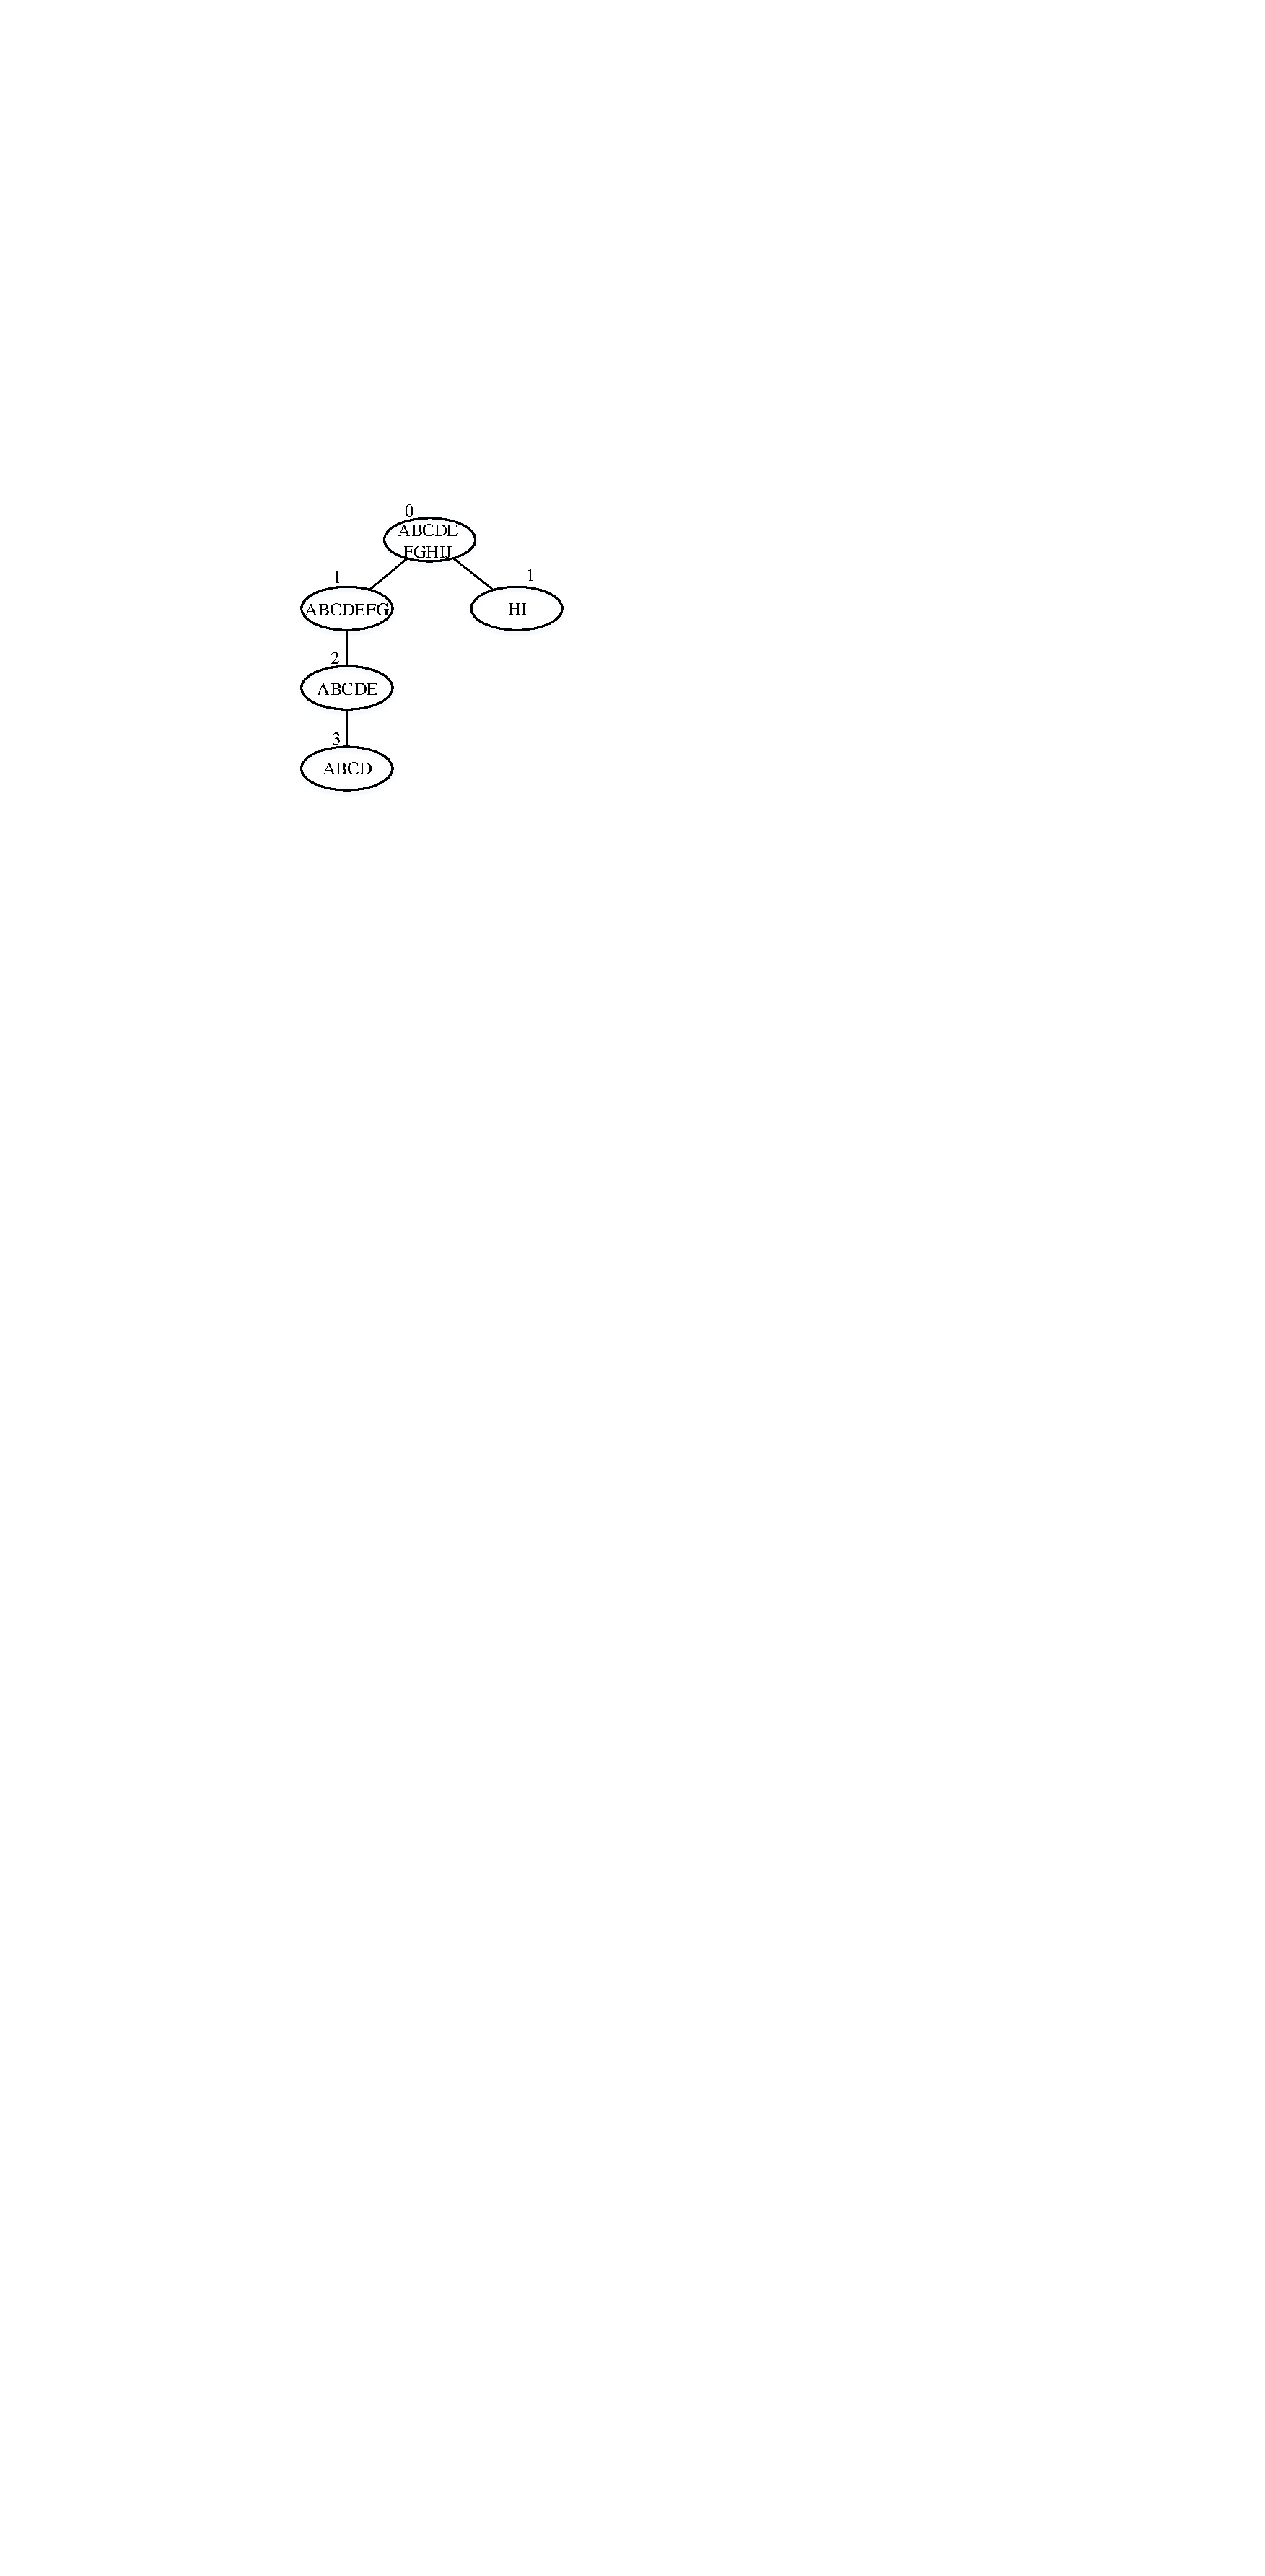
\includegraphics[width=.375\columnwidth]{figures/uck-tree}
            \label{fig:ucktree}
        }
        \hspace{2ex}
        \subfigure[CL-tree index]{
            
\includegraphics[width=.45\columnwidth]{figures/ck-tree}
            \label{fig:cktree}
        }
    }
    \caption{An example CL-tree index.}\label{fig:index}
\end{figure}

The tree structure in Figure~\ref{fig:ucktree} can be stored compactly, as shown in Figure~\ref{fig:cktree}.
The key observation is that, for any internal node $p$ in the tree,
the vertex sets of its child nodes are the subsets of $p$'s vertex set,
because of the inclusion relationship. To save space cost,
we can remove the redundant vertices that are shared by $p$'s child nodes from $p$'s vertex set.
After such removal, we obtain a compressed tree,
where each graph vertex appears only once.
This structure constitutes the CL-tree index, the nodes of which are further augmented by inverted lists (Figure~\ref{fig:cktree}).
For each keyword $e$ that appears in a CL-tree node, a list of IDs of vertices whose keyword sets contain $e$ is stored.  For example, in node $r_3$, the inverted list of keyword $y$ contains $\{A,C,D\}$. As discussed later, given a keyword set $T$, these inverted lists allow efficient retrieval of vertices whose keyword sets contain $T$.
To summarize, each CL-tree node contains five elements:

$\bullet$ \emph{coreNum}: the core number of the $k$-$\widehat {core}$;

$\bullet$ \emph{vertexSet}: a set of graph vertices;

$\bullet$ \emph{invertedList}: a list of $\textless key,value\textgreater$ pairs, where the $key$ is a keyword contained by vertices in $vertexSet$ and the $value$ is the list of vertices in $vertexSet$ containing $key$;

$\bullet$ \emph{childList}: a list of child nodes.

\chen{
$\bullet$ \emph{fatherNode}: the father node of the current node.
}

Figure~\ref{fig:cktree} depicts the CL-tree index for the example graph in Figure~\ref{fig:kcoreGraph},
the elements of each tree node are labeled explicitly.
Using the CL-tree, the following two key operations used by our query algorithms (Section~\ref{query}), can be performed efficiently.

$\bullet$ {\bf{Core-locating.}} Given a vertex $q$ and a core number $c$,
	find the $k$-$\widehat {core}$ with core number $c$ containing $q$,
	by traversing the CL-tree.
	
$\bullet$ {\bf{Keyword-checking.}} Given a $k$-$\widehat {core}$, find vertices which contain a given keyword set, by intersecting the inverted lists of keywords contained in the keyword set.


\textbf{Remarks.}
The CL-tree can also support $k$-$\widehat {core}$ queries on general graphs without keywords.
For example, it can be applied to finding $k$-$\widehat{core}$ in previous community search methods~\cite{KDD2010}.


\textbf{Space cost.}
Since each graph vertex appears only once and each keyword only needs constant space cost,
the space cost of keeping such an index is $O({\widehat l}\cdot n)$,
where $\widehat l$ denotes the average size of $W(v)$ over $V$.
Thus, the space cost is linear to the size of $G$. 
\subsection{Index Construction}
\label{indexConstruction}
To build the CL-tree index, we propose two methods, {\tt basic} and {\tt advanced},
as presented in Section~\ref{basicIndex} and~\ref{advancedIndex}.

\subsubsection{The Basic Method}
\label{basicIndex}
As $k$-$\widehat {core}$s of a graph are nested naturally,
it is straightforward to build the CL-tree recursively in a top-down manner.
Specifically, we first generate the root node for $0$-core, which is exactly the entire graph.
Then, for each $k$-$\widehat {core}$ of $1$-core, we generate a child node for the root node.
After that, we only remain vertices with core numbers being $0$ in the root node.
Then for each child node, we can generate its child nodes in the similar way.
This procedure is executed recursively until all the nodes are well built.

\begin{algorithm}[h]
\caption{Index construction: {\tt basic}}
\label{alg:basicIndex}
\footnotesize{
\algrenewcommand{\algorithmiccomment}[1]{\hskip3em$//$ #1}
\begin{algorithmic}[1]
    \Function{buildIndex($G(V,E)$)}{}
        \State $core_G[\text{ }]\gets$ $k$-core decomposition on $G$;
        \State $k\gets$0, $root\gets (k, V)$;
        \State \Call{buildNode($root$, $0$)}{};
        \State build an inverted list for each tree node;
        \State \Return $root$;
    \EndFunction
    \Function{buildNode($root$, $k$)}{}
        \State $k\gets k+1$;
        \If{$k\leq k_{max}$}
            \State obtain $U_k$ from $root$;
            \State compute the connected components for the induced graph on $U_k$;
            %\luo{Do you mean "the connected components for the induced graph on $U_k$"?}
            \For {each connected component $C_i$}
                \State build a tree node $p_i\gets (k, C_i.vertexSet)$;
                \State add $p_i$ into $root.childList$;
                \State remove $C_i$'s vertex set from $root.vertexSet$;
                \State \Call{buildNode($p_i$, $k$)}{};
            \EndFor
        \EndIf
    \EndFunction
\end{algorithmic}}
\end{algorithm}


Algorithm~\ref{alg:basicIndex} illustrates the pseudocodes.
We first do $k$-core decomposition
using the linear algorithm~\cite{kcore2003},
and obtain an array $core_G[\text{ }]$(line 2),
where $core_G[i]$ denotes the core number of vertex $i$ in $G$.
We denote the maximal core number by $k_{max}$.
Then, we initialize the root node by the core number $k$=0 and $V$ (line 3).
Next, we call the function \textsc{buildNode} to build its child nodes (line 4).
Finally, we build an inverted list for each tree node and
obtain a well built CL-tree (lines 5-6).

In \textsc{buildNode}, we first update $k$ and obtain the vertex set $U_k$ from $root.vertexSet$,
which is a set of vertices with core numbers being at least $k$.
Then we find all the connected components from the subgraph induced by $U_k$ (lines 8-11).
Since each connected component $C_i$ corresponds to a $k$-$\widehat {core}$,
we build a tree node $p_i$ with core number $k$ and the vertex set of $C_i$,
and then link it as a child of $root$ (lines 12-14).
We also update $root$'s vertex set by removing vertices (line 15),
which are shared by $C_i$.
Finally, we call the \textsc{buildNode} function to build $p_i$'s child nodes recursively until all the tree nodes are created (line 16).

\textbf{Complexity analysis.}
The $k$-core decomposition can be done in $O(m)$.
The inverted lists of each node can be built in $O({\widehat l}\cdot n)$.
In function \textsc{buildNode}, we need to compute the connected components with a given vertex set,
which costs $O(m)$ in the worst case.
Since the recursive depth is $k_{max}$, the total time cost is $O(m\cdot {k_{\max }}+{\widehat l}\cdot n)$.
Similarly, the space complexity is $O(m+{\widehat l}\cdot n)$.

\subsubsection{The Advanced Method}
\label{advancedIndex}
While the {\tt basic} method is easy to implement,
it meets efficiency issues when both the given graph size and its $k_{max}$ value are large.
For instance, when given a clique graph with $n$ vertices (\textit{i.e.}, edges exist between every pair of nodes),
the value of $k_{max}$ is $n$--1. Therefore, the time complexity of the {\tt basic} method could be $O((m+{\widehat l})\cdot n)$,
which may lead to low efficiency for large-scale graphs.
To enable more efficient index construction, we propose the {\tt advanced} method,
whose time and space complexities are almost linear with the size of the input graph.

The {\tt advanced} method builds the CL-tree level by level in a bottom-up manner. Specifically, the tree nodes corresponding to larger core numbers are created prior to those with smaller core numbers. For ease of presentation, we divide the discussion into two main steps: creating tree nodes and creating tree edges.

\textbf{1. Creating tree nodes.} We observe that, if we acquire the vertices with core numbers at least $c$ and denote the induced subgraph on the vertices as $T_c$, then the connected components of $T_c$ have one-to-one correspondence to the $c$-$\widehat {core}$s. A simple algorithm would be, searching connected components for $T_c (0\leq c\leq k_{max})$ independently, followed by creating one node for each distinct component. This algorithm apparently costs $O(k_{max}\cdot m)$ time, as computing connected components takes linear time.
% given that the connected component search for a graph can be completed in linear time.

However, we can do better if we can incrementally update the connected components in a level by level manner (\textit{i.e.}, maintain the connected components of $T_{c+1}$ from those of $T_{c}$). We note that, such a node creation process is feasible by exploiting the classical \emph{union-find forest}~\cite{unionFind}. Generally speaking, the union-find forest enables efficient maintenance of connected components of a graph when edges are incrementally added. Using union-find forest to maintain connected components follows a process of edge examination. Initially, each vertex is regarded as a connected component. Then, edges are examined one by one. During the examine process, two components are merged together when encounters an edge connecting them. To achieve an efficient merge of components, the vertices in the component form a tree. The tree root acts as the representative vertex of the component. As such, merging two components is essentially linking two root vertices together. To guarantee the CL-tree nodes are formed in a bottom-up manner, we assign an examine priority to each edge. The priority is defined by the larger value of the two core numbers corresponding to the two end vertices of an edge. The edges associated to vertices with larger core numbers are examined first.

\textbf{2. Creating tree edges.} Tree edges are also inserted during the graph edge examination process.
In particular, when we examine a vertex $v$ with a set, $B$, of its neighbors, whose core numbers are larger than $core_G[v]$,
we require that the tree node containing $v$ should link to the tree node containing
the vertex, whose core number is the smallest among all the vertices in $B$.
Nevertheless, the classical union-find forest is not able to maintain such information. To address this issue, we thus propose an auxiliary data structure,
called \textbf{\underline{A}nchored \underline{U}nion-\underline{F}ind} (details of AUF are in Appendix~\ref{app:auf}),
based on the classical union-find forest.
We first define \emph{anchor vertex}.


\begin{definition}[Anchor vertex]
\label{def:anchor}
Given a connected subgraph $G'\subseteq G$,
the anchor vertex is the vertex with core number being $min\{core_G[v]|v\in G'\}$.
\end{definition}

The AUF is an extension of union-find forest, in which each tree has an anchor vertex,
and it is attached to the root node.
In CL-tree, for any node $p$ with corresponding $k$-$\widehat {core}$ ${\mathcal C}_k$,
its child nodes correspond to the $k$-$\widehat {core}$s,
which are contained by ${\mathcal C}_k$ and have core numbers being the most close to the core number of node $p$.
This implies that, when building the CL-tree in a bottom-up manner,
we can maintain the anchor vertices for the $k$-$\widehat {core}$s dynamically,
and they can be used to link nodes with their child nodes.
In addition, we maintain a vertex-node map,
where the key is a vertex and the value is the tree node contains this vertex,
for locating tree nodes.

\begin{algorithm}[h]
\caption{Index construction: {\tt advanced}}
\label{alg:advancedIndex}
\footnotesize{
\algrenewcommand{\algorithmiccomment}[1]{\hskip3em$//$ #1}
\begin{algorithmic}[1]
\Function{buildIndex($G(V,E)$)}{}
        \State $core_G[\text{ }]\gets$ $k$-core decomposition on $G$;
        \For {each $v\in V$}
            \Call{makeSet($v$)}{};
        \EndFor
        \State put vertices into sets $V_0, V_1, \cdots, V_{k_{max}}$;
        \State $k\gets k_{max}$, $map\gets \emptyset$;
        \While {$k\geq 0$}
            \State $V'\gets \emptyset$;
            \For {each $v\in V_k$}
                $V'$.add(\Call{find($v$)}{});
            \EndFor
            \State compute connected components for $V_{k}\cup V'$;
            \For {each component with vertex set $C_i$}
                \State create a node $p_i$ using ($k$, $\{C_i-V'\}$);
                \For {each $v \in \{C_i-V'\}$}
                    %\State $invertArr[v]\gets p_i$;
                    \State $map$.add($v$, $p_i$);
                    \For {each $ u \in v$'s neighbor vertices}
                        \If {$core_G[u]\geq core_G[v]$}
                            \State \Call{union($u$, $v$)}{};
                        \EndIf
                        \If {$core_G[u]>core_G[v]$}
                            \State $uRoot\gets$\Call{find($u$)}{};
                            \State $uAnchor\gets uRoot.anchor$;
                            %\State $p'\gets invertArr(uAnchor)$;
                            \State $p'\gets$ $map$.get($uAnchor$);
                            \State add $p'$ to $p$'s child List;
                        \EndIf
                    \EndFor
                    \State $vRoot\gets$\Call{find($v$)}{};
                    \If {$core_G[vRoot.anchor] > core_G[v]$}
                        \State \Call{updateAnchor($vRoot$, $core_G[\text{ }]$, $v$)}{};
                    \EndIf
                \EndFor
            \EndFor
            \State $k\gets k-1$;
        \EndWhile
        \State build the root node $root$;
        \State build an inverted list for each tree node;
        \State \Return $root$.
\EndFunction
\end{algorithmic}}
\end{algorithm}

Algorithm~\ref{alg:advancedIndex} presents the {\tt advanced} method.
Similar with {\tt basic} method, we first conduct $k$-decomposition (line 2).
Then, for each vertex, we initialize an AUF tree node (line 3).
We group all the vertices into sets (line 4),
where set $V_k$ contains vertices with core numbers being exactly $k$ (line 5).
Next, we initialize $k$ as $k_{max}$ and the vertex-node map $map$,
where the key is a vertex and the value is a CL-tree node whose vertex set contains this vertex.
In the while loop (lines 6-25),
we first find the set $V'$ of the representatives for vertices in $V_k$,
then compute the connected components for vertex set $V_k\cup V'$ (lines 7-9).
Next, we create a node $p_i$ for each component (lines 10-11).
For each vertex $v\in \{C_i-V'\}$, we add a pair ($v$, $p_i$) to the $map$ (lines 12-13).
Then for each of $v$'s neighbor, $u$, if its core number is at least $core_G[v]$,
we link $u$ and $v$ together in the AUF by a \textsc{union} operation (lines 14-16),
and find $p_i$'s child nodes using the anchor of the AUF tree (lines 17-21).
After vertex $v$ has been added into the CL-tree, we update the anchor (lines 22-24).
Then we move to the upper level in next loop (line 25).
After the while loop, we build the root node of the CL-tree (line 26).
Finally, we build the inverted list for each tree node and obtain the built index (lines 27-28).


\textbf{Complexity analysis.}
In Algorithm~\ref{alg:advancedIndex}, lines 1-3 can be completed in $O(m)$ (We assume $m$>$n$).
In the while loop, the number of operations on each vertex and its neighbors are constant,
and each can be done in $O(\alpha(n))$, where $\alpha(n)$ is the inverse Ackermann function.
The keyword inverted lists of all the tree nodes can be computed in $O(n\cdot {\widehat l})$.
Therefor, the CL-tree can be built in $O(m\cdot \alpha(n)+n\cdot{\widehat l})$.
The space cost is $O(m+n\cdot{\widehat l})$, as maintaining an AUF takes $O(n)$.

%\textbf{Complexity analysis.}
%With our proposed AUF, we can reduce the complexity of CL-tree construction to $O(m\cdot \alpha(n))$,
%%which conforms to the complexity analysis of the classical union-find forest~\cite{unionFind}.
%where $\alpha(n)$, the inverse Ackermann function, is less than 5 for all remotely practical
%values of $n$~\cite{unionFind}.

\begin{example}
Figure~\ref{fig:advancedIndex} depicts an example graph with 14 vertices {$A,\cdots,N$}.
$V_i$ denotes the set of vertices whose core numbers are $i$.
When $k$=3, we first generate two leaf nodes $p_1$ and $p_2$,
then update the AUF, where roots' anchor vertices are in the round brackets.
When $k$=2, we first generate node $p_3$, then link it to $p_1$,
and then update the AUF forest.
When $k$=1, we first generate nodes $p_4$ and $p_5$.
Specifically, to find the child nodes of $p_4$,
we first find its neighbor $A$,
then find $A$'s parent $B$ using current AUF forest.
Since the anchor vertex of $B$ is $E$ and $E$ points to $p_3$ in the inverted array,
we add $p_3$ into $p_4$'s child List.
When $k$=0, we generate $p_6$ and finish the index construction.
\end{example}

\begin{figure}
	\small
	\centering
	
\includegraphics[width=0.85\linewidth]{figures/advancedIndex}
	\caption{An index built by {\tt advanced} method.}
	\label{fig:advancedIndex}
\end{figure} 



\section{Query Algorithms}
\label{query}

In this section, we present three query algorithms based on the CL-tree index.
Based on how we verify the candidate keyword sets, we divide our algorithms into incremental algorithms (from examining smaller candidate sets to larger ones) and decremental algorithm (from examining larger candidate sets to smaller ones).
We propose two incremental algorithms called \textbf{{\tt Inc-S}} (\underline{Inc}remental \underline{S}pace efficient) and \textbf{{\tt Inc-T}} (\underline{Inc}remental \underline{T}ime efficient), to trade off between the memory consumption and the computational overhead.
The decremental algorithm is called \textbf{{\tt Dec}} (\underline{Dec}remental).
Our interesting finding is that, while {\tt Dec} seems not intuitive, it ranks as the most efficient one.
{\tt Inc-S} and {\tt Inc-T} are presented in Section~\ref{inc}.
{\tt Dec} is introduced in Section~\ref{dec}.

\subsection{The Incremental Algorithms}
\label{inc}

While the high-level idea of incremental algorithms resembles the basic solutions (see Section~\ref{basic}),
{\tt Inc-S} and {\tt Inc-T} advance them with the exploitation of the CL-tree.
Specifically, they can always verify the existence of $G_k[S']$ within a subgraph of $G$ instead of the entire graph $G$. More interestingly, the subgraph for such verifications shrinks when the candidate set $S'$ expands. Therefore, a large sum of redundant computation is cut off during the verification. We present {\tt Inc-S} and {\tt Inc-T} in Sections~\ref{inc-S} and~\ref{inc-T}.


\subsubsection{Inc-S Algorithm}
\label{inc-S}
We first introduce a new concept, called \textbf{subgraph core number},
which is geared to the main idea of {\tt Inc-S}.

\begin{definition}[Subgraph core number]
\label{def:ccscore}
  The core number of a subgraph $G'$ of $G$, $core_G[G']$,
  is defined as $min\{core_G[v]|$ $v\in G'\}$.
\end{definition}


{\tt Inc-S} follows the two-step framework (\emph{verification} and \emph{candidate generation})
introduced in Section~\ref{basic}. With the CL-tree, we improve the verification step as follows.
\begin{itemize}
\item {\bf Core-based verification.} For each newly generated size-($c$+1) candidate keyword set $S'$ expanded from size-$c$ sets $S_1$ and $S_2$, mark $S'$ as a qualified set if $G_k[S']$ exists \textit{in a subgraph of core number} $max\{core_G[G_k[S_1]]$, $core_G[G_k[S_2]]\}$.
\end{itemize}

The core-based verification guarantees that, with the expansion of the candidate keyword sets, the verification becomes faster as it only needs to examine the existence of $G_k[S']$ in a smaller $k$-$\widehat {core}$ (Recall that cores with large core numbers are nested in the cores with small core numbers). The correctness of such shrunk verification range is guaranteed by the following lemma.
\begin{lemma}
\label{lemma:coreDown}
  Given two subgraphs $G_k[S_1]$ and $G_k[S_2]$ of a graph $G$,
  for a new keyword set $S'$ generated from $S_1$ and $S_2$ (\textit{i.e.}, $S'=S_1\cup S_2$),
  if $G_k[S']$ exists, then it must appear in a $k$-$\widehat {core}$ with core number at least
  \begin{equation}
    max\{core_G[G_k[S_1]], core_G[G_k[S_2]]\}.
  \end{equation}
\end{lemma}

The verification process can be further accelerated by checking the numbers of vertices and edges,
as indicated by Lemma~\ref{lemma:coreExist}.
\begin{lemma}
\label{lemma:coreExist}
  Given a connected graph $G(V,E)$ with $n$=$|V|$ and $m$=$|E|$,
  if $m - n < \frac{{{k^2} - k}}{2} - 1$, there is no $k$-$\widehat {core}$ in $G$.
\end{lemma}

This lemma implies that, for a connected subgraph $G'$, whose edge and vertex numbers are $m$ and $n$,
if $m - n < \frac{{{k^2} - k}}{2} - 1$, then we cannot find $G_k[S']$ from $G'$.

We present {\tt Inc-S} in Algorithm~\ref{alg:incS}.
The input is a CL-tree rooted at $root$, a query vertex $q$, a positive integer $k$ and a keyword set $S$.
We apply {\tt core-locating} on the CL-tree to locate the internal nodes whose corresponding $k$-$\widehat {core}$s contain $q$ (line 2).
Note that their core numbers are in the range of $[k,core_G[q]]$, as required by the structure cohesiveness.
Then, we set $l$=0, indicating the sizes of current keyword sets, and initialize a set $\Psi$ of $\textless S',c\textgreater$ pairs,
where $S'$ is a set containing a keyword from $S$ and $c$ is the initial core number $k$ (line 3).
Note that we skip those keywords, which are in $S$, but not in $W(q)$.
In the while loop (lines 4-18), for each $\textless S',c\textgreater$ pair,
we first perform {\tt keyword-checking} to find $G[S']$ using the keyword inverted lists of the subtree rooted at node $r_c$.
If we cannot ensure that $G[S']$ does not contain a $k$-$\widehat {core}$ by Lemma~\ref{lemma:coreExist},
we then find $G_k[S']$ from $G[S']$ (lines 8-9).
If $G_k[S']$ exists, we put $S'$ with its core number into the set $\Phi_l$ (lines 10-11).
Next, if $\Phi_l$ is nonempty, we generate new candidates by calling \textsc{geneCand($\Phi_{l}$)},
which is detailed in Appendix~\ref{app:geneCand}.
For each candidate $S'$ in $\Psi$, we compute the core number using Lemma~\ref{lemma:coreDown}
and update it as a pair in $\Psi$ (lines 12-17);
otherwise, we stop (line 18).
Finally, we output the communities of the latest verified keyword sets (line 19).

\begin{algorithm}[h]
\caption{Query algorithm: {\tt Inc-S}}
\label{alg:incS}
\footnotesize{
\algrenewcommand{\algorithmiccomment}[1]{\hskip3em$//$ #1}
\begin{algorithmic}[1]
    \Function{query($G$, $root$, $q$, $k$, $S$)}{}
        \State find subtree root nodes $r_k,r_{k+1},\cdots,r_{core_G[q]}$;
        \State initialize $l$=0, $\Psi$ using $S$;
        \While{$true$}
            \State $l\gets l+1$; $\Phi_{l} \gets \emptyset$;
            \For {each $\textless S',c \textgreater$ $\in \Psi$}
                \State find $G[S']$ under the root $r_c$;
                \If {$G[S']$ is not pruned by Lemma~\ref{lemma:coreExist}}
                    \State find $G_k[S']$ from $G[S']$;
                    \If {$G_k[S']$ exists}
                        \State $\Phi_{l}$.add($\textless S', core_G[G_k[S']]\textgreater$);
                    \EndIf
                \EndIf
            \EndFor

            \If{$\Phi_{l} \ne \emptyset$}
                \State $\Psi \gets$ \Call{geneCand($\Phi_{l}$)}{};
                \For {each $S'$ in $\Psi$}
                    \If {$S'$ is generated from $S_1$ and $S_2$}
                        \State $c\gets max\{core_G[G_k[S_1]],core_G[G_k[S_2]]\}$;
                        \State $\Psi$.update($S'$, $\textless S',c\textgreater$);
                    \EndIf
                \EndFor
            \Else {} break;
            \EndIf
        \EndWhile
        \State output the communities of keyword sets in $\Phi_{l-1}$;
    \EndFunction
\end{algorithmic}}
\end{algorithm}

\begin{example}
\label{eg:inc-S}
Consider the graph in Figure~\ref{fig:kcoreGraph}
and its index in Figure~\ref{fig:cktree}.
Let $q$=$A$, $k$=1 and $S$=$\{w,x,y\}$.
By Algorithm~\ref{alg:incS}, we first find 3 root nodes $r_1$, $r_2$ and $r_3$.
In the first while loop, we find 2 qualified keyword sets $\{x\}and \{y\}$ with core numbers being 3 and 1.
By Lemma~\ref{lemma:coreDown}, we only need to verify the new candidate keyword set $\{x,y\}$ under node $r_3$.
\end{example}

\subsubsection{Inc-T Algorithm}
\label{inc-T}
We begin with a lemma which inspires the design of {\tt Inc-T}.
\begin{lemma}
\label{lemma:kcoreIntersect}
  Given two keyword sets $S_1$ and $S_2$, if $G_k[S_1]$ and $G_k[S_2]$ exist, we have
  \begin{equation}
    %{G_k}[{S_1} \cup {S_2},q] \subseteq {G_k}[{S_1},q] \cap {G_k}[{S_2},q].
    G_k[S_1\cup S_2] \subseteq G_k[S_1]\cap G_k[S_2].
  \end{equation}
\end{lemma}

This lemma implies, if $S'$ is generated from $S_1$ and $S_2$,
we can find $G_k[S']$ from $G_k[S_1]\cap G_k[S_2]$ directly.
Since every vertex in $G_k[S_1]\cap G_k[S_2]$ contains both $S_1$ and $S_2$,
we do not need to consider the keyword constraint again when finding $G_k[S']$.

Based on Lemma~\ref{lemma:kcoreIntersect}, we introduce a new algorithm \textbf{{\tt Inc-T}}. Different from {\tt Inc-S}, {\tt Inc-T} maintains $G_k[S']$ rather than $core_G[$ $G_k[S']]$ for each qualified keyword set $S'$. As we will demonstrate later, {\tt Inc-T} is more effective for shrinking the subgraphs containing the ACs, and thus more efficient. As a trade-off for better efficiency, {\tt Inc-T} consumes more memory as it needs to store a list of subgraph $G_k[S']$ in memory.

\begin{algorithm}[h]
\caption{Query algorithm: {\tt Inc-T}}
\label{alg:incT}
\footnotesize{
\algrenewcommand{\algorithmiccomment}[1]{\hskip3em$//$ #1}
\begin{algorithmic}[1]
    \Function{query($G$, $root$, $q$, $k$, $S$)}{}
        \State find the $k$-$\widehat {core}$, which contains $q$;
        \State initialize $l$=0, $\Psi$ using $S$;
        \While{$true$}
            \State $l\gets l+1$; $\Phi_{l} \gets \emptyset$;
            \For {each $<S',\widehat{G}>$ $\in \Psi$}
                \State find $G[S']$ from $\widehat{G}$;
                \If {$G[S']$ is not pruned by Lemma~\ref{lemma:coreExist}}
                    \State find $G_k[S']$ from $G[S']$;
                    \If {$G_k[S']$ exists}
                        \State $\Phi_{l}$.add($<S', G_k[S']>$);
                    \EndIf
                \EndIf
            \EndFor
            \If {$\Phi_{l} \ne \emptyset$}
                \State $\Psi \gets$ \Call{geneCand($\Phi_{l}$)}{};
                \For {each $S' \in \Psi$}
                    \If {$S'$ is generated from $S_1$ and $S_2$}
                        \State $\widehat G \gets G_k[S_1]\cap G_k[S_2]$;
                        \State $\Psi_{l}$.update($S'$,$<S',\widehat G>$);
                   \EndIf
                \EndFor
            \Else {} break;
            \EndIf
        \EndWhile
        \State output the communities of keyword sets in $\Phi_{l-1}$;
    \EndFunction
\end{algorithmic}}
\end{algorithm}

Algorithm~\ref{alg:incT} presents the steps of {\tt Inc-T}.
We first apply {\tt core-locating} to find the $k$-$\widehat{core}$ containing $q$ from the CL-tree (line 2).
Then, we set $l$=0, indicating the sizes of current keyword sets,
and initialize a set $\Psi$ of $<S',\widehat G>$ pairs,
where $S'$ is a set containing a keyword from $S$ and $\widehat G$ is the $k$-$\widehat {core}$.
The while loop (lines 4-18) is similar with that of {\tt Inc-S}.
The main differences are that:
(1) for each qualified keyword set $S'$, {\tt Inc-T} keeps $G_k[S']$ in memory (line 11);
and (2) for each candidate keyword set $S'$ generated from $S_1$ and $S_2$,
{\tt Inc-T} finds $G_k[S']$ from $G_k[S_1]\cap G_k[S_2]$ directly without further keyword verification (lines 6-9, 16).

\begin{example}
\label{eg:inc-T}
Continue the graph and query ($q$=$A$, $k$=1, $S$=$\{w$, $x,y\}$) in Example~\ref{eg:inc-S}.
By {\tt Inc-T}, we first find $G_1[\{x\}]$ and $G_1[\{y\}]$,
whose vertex sets are $\{A,B,C,D\}$ and $\{A,C,D$, $E,F,G\}$.
Then to find $G_1[\{x,y\}]$, we only need to search it from the subgraph,
induced by the vertex set $\{A,C,D\}$.
\end{example}




\subsection{The Decremental Algorithm}
\label{dec}

The decremental algorithm, denoted by {\tt Dec}, differs from previous query algorithms
not only on the generation of candidate keyword sets,
but also on the verification of candidate keyword sets.

\textbf{1. Generation of candidate keyword sets.}
{\tt Dec} exploits the key observation that,
if $S'$ ($S'\subseteq S$) is a qualified keyword set,
then there are at least $k$ of $q$'s neighbors containing set $S'$.
This is because every vertex in $G_k[S']$ must has degree at least $k$.
This observation implies,
we can generate all the candidate keyword sets directly by using the query vertex $q$ and $q$'s neighbors,
without touching other vertices.

Specifically, we consider $q$ and $q$'s neighbor vertices.
For each vertex $v$, we only select the keywords, which are contained by $S$ and at least $k$ of its neighbors.
Then we use these selected keywords to form an itemset, in which each item is a keyword.
After this step, we obtain a list of itemsets.
Then we apply the well studied frequent pattern mining algorithms
(e.g., Apriori~\cite{han2011data} and FP-Growth~\cite{han2000mining})
to find the frequent keyword combinations,
each of which is a candidate keyword set.
Since our goal is to generate keyword combinations shared by at least $k$ neighbors,
we set the minimum support as $k$.
In this paper, we use the well-known FP-Growth algorithm~\cite{han2000mining}.

\begin{figure}[ht]
    \centering
    \mbox{
        \subfigure[a query vertex]{
            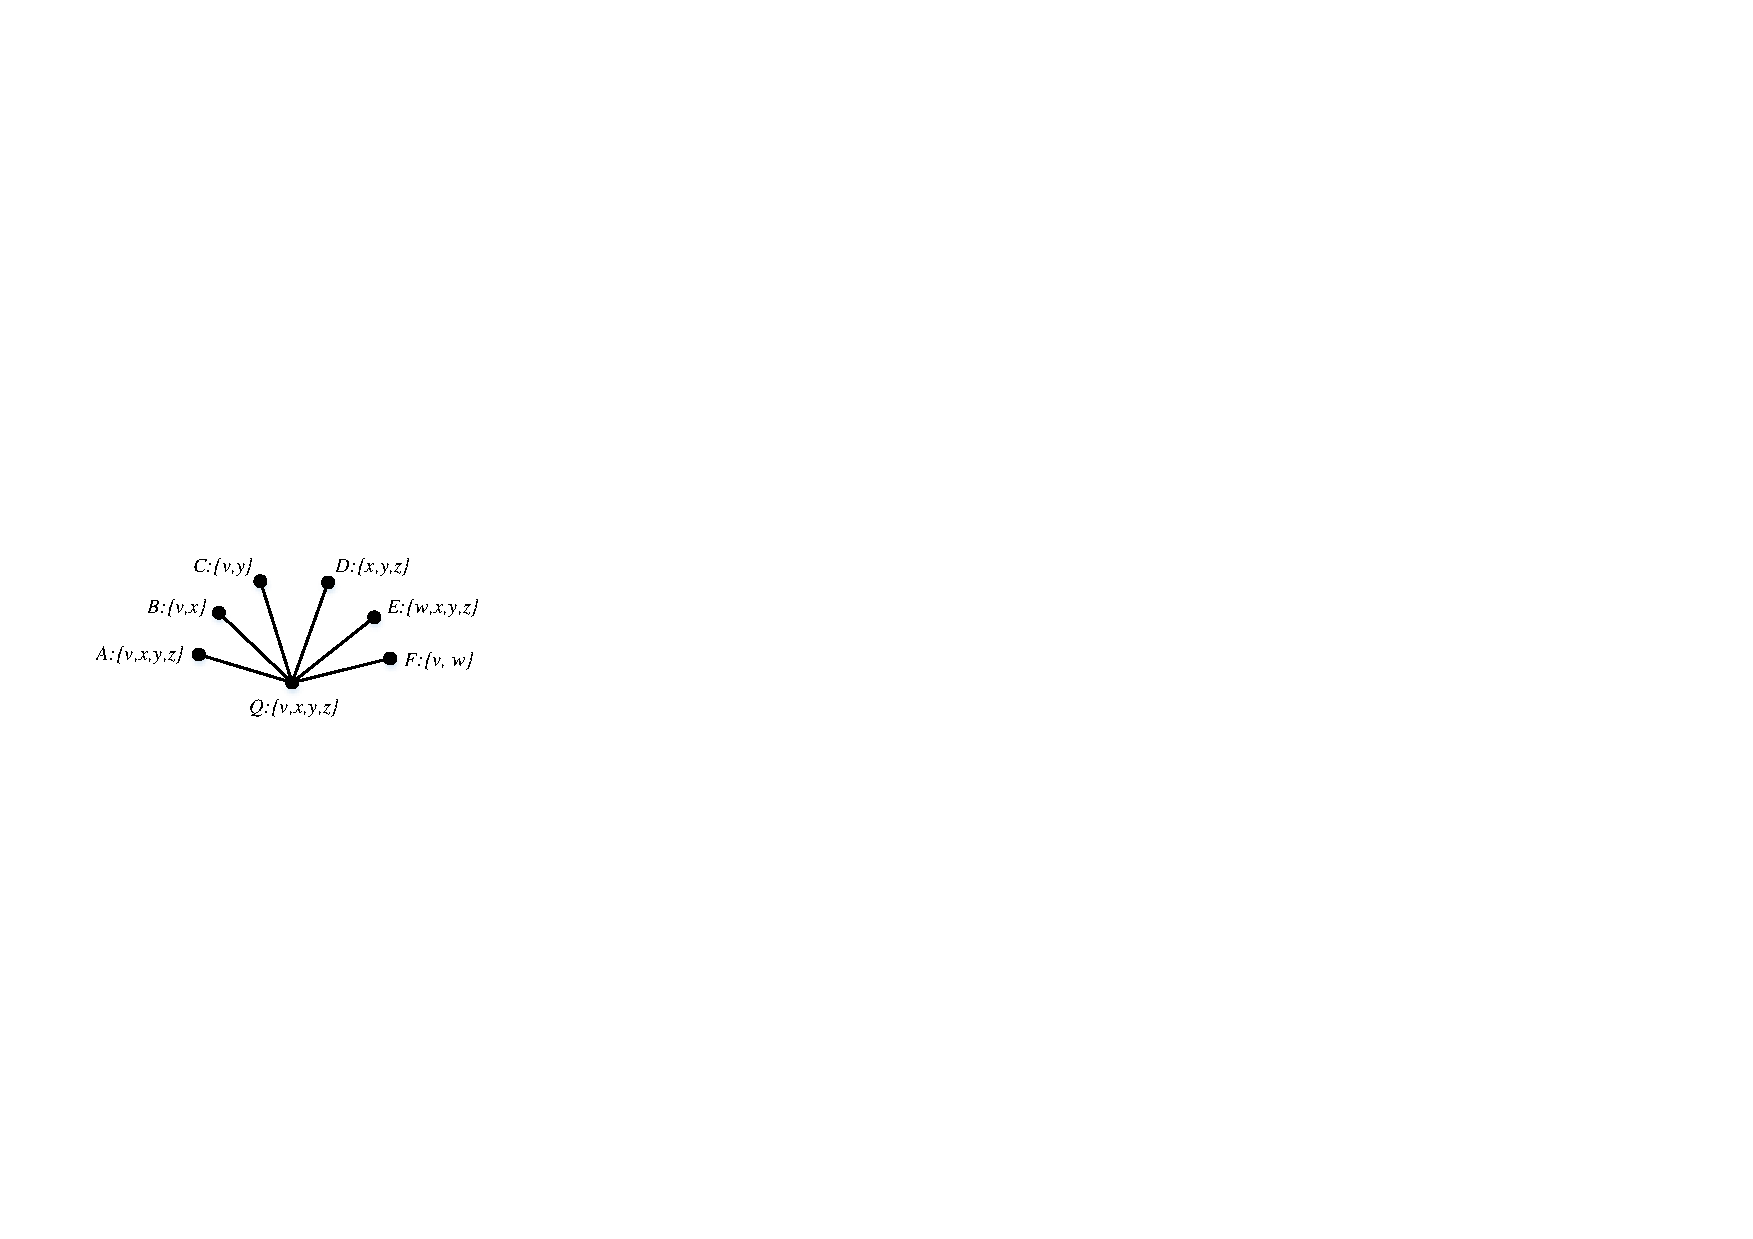
\includegraphics[width=.51\columnwidth]{figures/nghGraph}
            \label{fig:nghGraph}
        }
        \hspace{1ex}
        \subfigure[candidates]{
            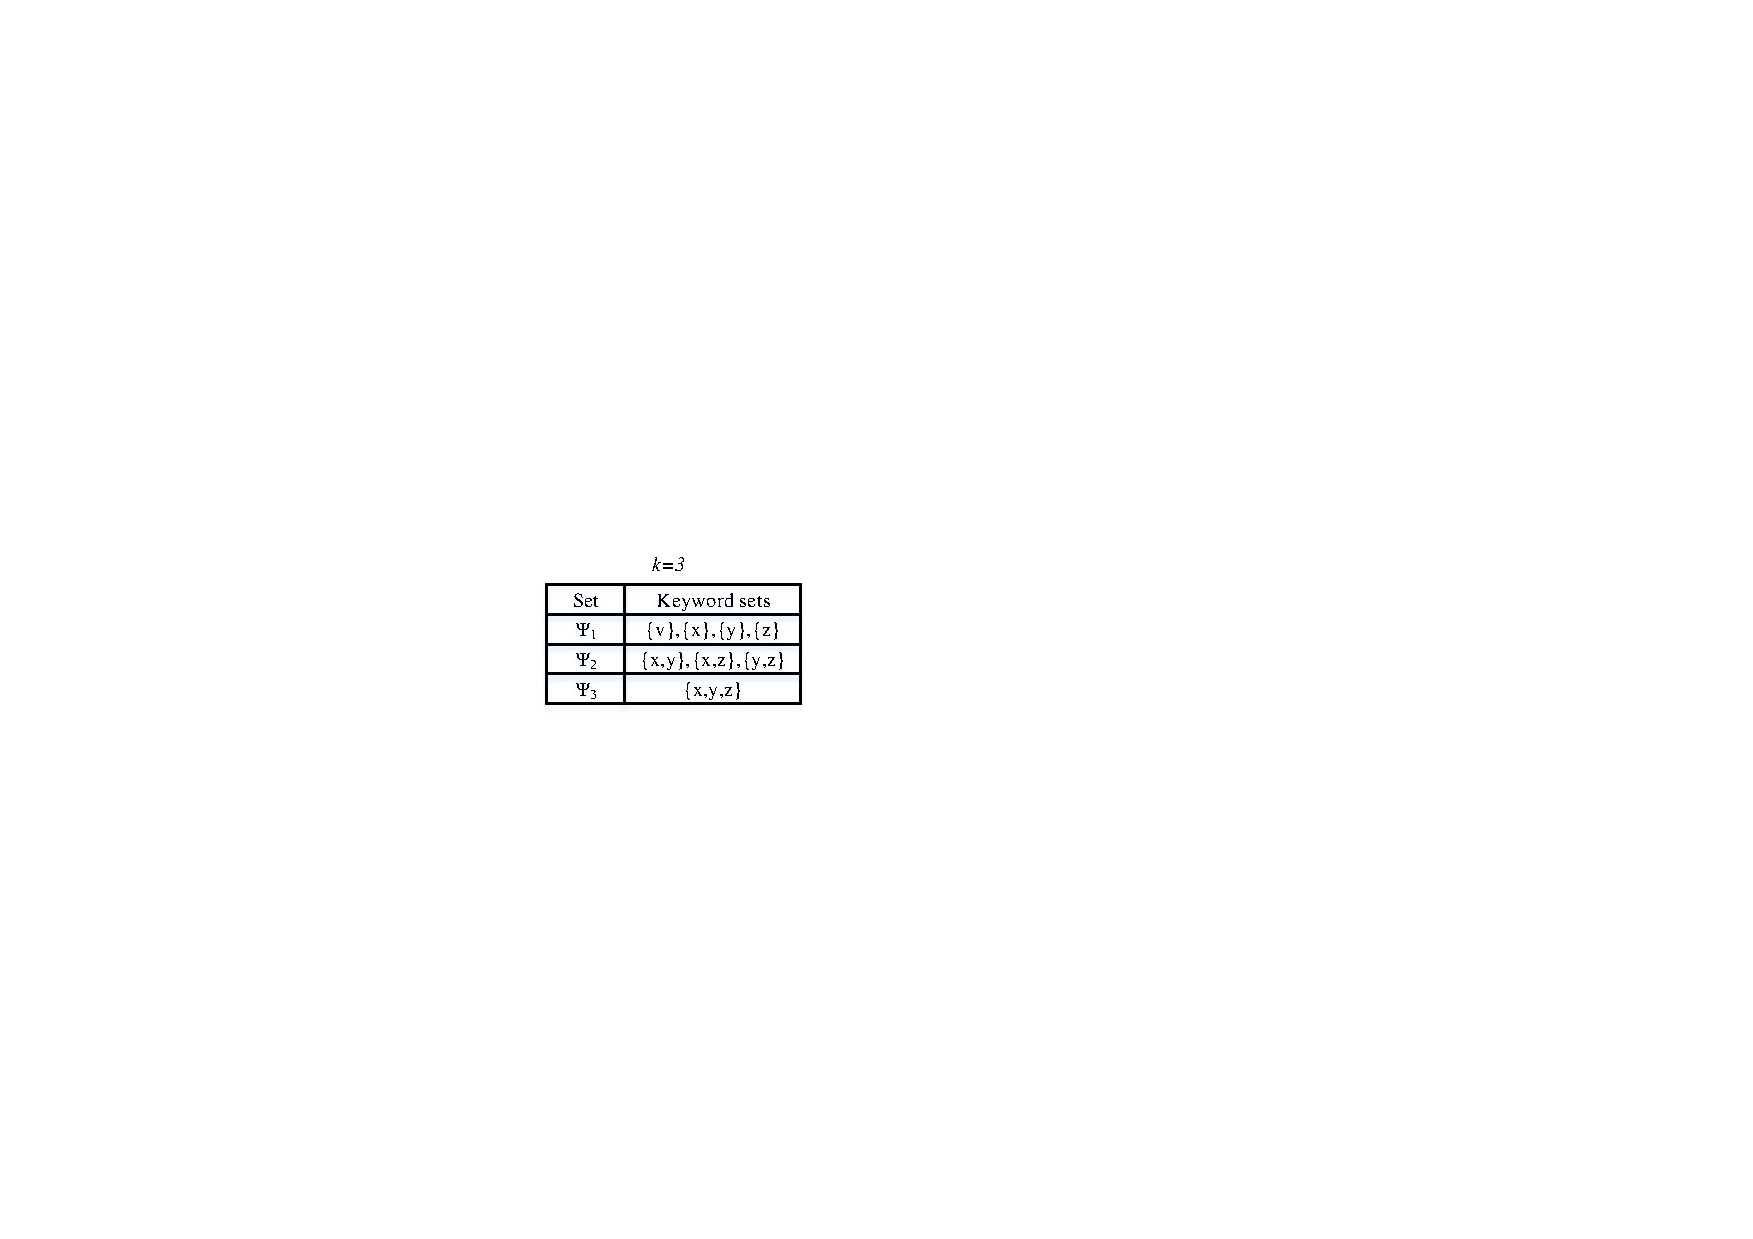
\includegraphics[width=.34\columnwidth]{figures/nghCand}
            \label{fig:nghCand}
        }
    }
    \caption{An example of candidate generation.}
\end{figure}
\begin{example}
Consider a query vertex $Q$ ($k$=3, $S$=$\{v,x,y,z\}$) with 6 neighbors in Figure~\ref{fig:nghGraph},
where the selected keywords of each vertex are listed in the curly braces.
By FP-Growth, 8 candidate keyword sets) are generated, as shown in Figure~\ref{fig:nghCand}.
$\Psi_i$ denotes the set of keyword sets with sizes being $i$.
\end{example}

\textbf{2. Verification of candidate keyword sets.}
As candidates can be obtained using $S$ and $q$'s neighbors directly,
we can verify them either incrementally as that in {\tt Inc-S},
or in a decremental manner (larger candidate keyword sets first and smaller candidate keyword sets later).
In this paper, we choose the latter manner. The rationale behind is that,
for any two keyword sets $S_1\subseteq S_2$, the number of vertices containing $S_2$ is usually smaller than that of $S_1$,
which implies $S_2$ can be verified more efficiently than $S_1$.

\begin{algorithm}[h]
\caption{Query algorithm: {\tt Dec}}
\label{alg:ngh}
\footnotesize{
\algrenewcommand{\algorithmiccomment}[1]{\hskip3em$//$ #1}
\begin{algorithmic}[1]
    \Function{query($G$, $root$, $q$, $k$, $S$)}{}
        \State generate $\Psi_1,\Psi_2,\cdots, \Psi_h$ using $S$ and $q$'s neighbors;
        \State find the subtree root node $r_k$;
        \State create $R_1,R_2,\cdots,R_{h'}$ by using subtree rooted at $r_k$;
        \State $l\gets h$; $Q\gets \emptyset$;
        \State ${\widehat R}\gets {R_h} \cup \cdots \cup {R_{h'}}$;
        \While {$l\geq 1$}
            \For {each $S'\in \Psi_l$}
                \State find $G[S']$ from the subgraph induced on $\widehat R$;
                \State find $G_k[S']$ from $G[S']$;
                \If {$G_k[S']$ exists}
                    $Q$.add($G_k[S']$);
                \EndIf
            \EndFor
            \If {$Q$=$\emptyset$}
                \State $l\gets l-1$;
                \State ${\widehat R}\gets {\widehat R}\cup R_l$;
            \Else {} break;
            \EndIf
        \EndWhile
        \State output communities in $Q$;
    \EndFunction
\end{algorithmic}}
\end{algorithm}

Based on the above discussions, we design {\tt Dec} as shown in Algorithm~\ref{alg:ngh}.
We first generate candidate keyword sets using $S$ and $q$'s neighbors by FP-Growth algorithm (line 2).
Then, we apply {\tt core-locating} to find the root (with core number $k$) of the subtree from CL-tree,
whose corresponding $k$-$\widehat {core}$ contains $q$ (line 3).
Next, we traverse the subtree rooted at $r_k$
and find vertices which share keywords with $q$ (line 4).
$R_i$ denote the sets of vertices sharing $i$ keywords with $q$.
Then, we initialize $l$ as $h$ (line 5),
as we verify keyword sets with the largest size $h$ first.
We maintain a set $\widehat R$ dynamically,
which contains vertices sharing at least $l$ keywords with $q$ (line 6).
In the while loop, we examine candidate keyword sets in the decremental manner.
For each candidate $S'\in\Psi_l$, we first try to find $G[S']$, then find $G_k[S']$,
and put $G_k[S']$ into $Q$ if it exists (lines 8-11).
Finally, if we have found at least one qualified community,
we stop at the end of this loop and output $Q$;
otherwise, we examine smaller candidate keyword sets in next loop.  

{\color{blue}
\section{Index Maintenance}
\label{indexMaintenance}

%In practice, the keywords and edges of graphs are often frequently updated.
In practice, the graphs are continuously evolving. Thus keywords and edges of graphs are often frequently updated.
Clearly, when the graph is updated, both the CL-tree index and the ACQ query results also need to be updated.
A straightforward method for handling the dynamic graph is to rebuild the index from scratch when an update is made.
However, this method is very inefficient, especially when the updates are very frequent.
To alleviate this issue, in this section we study how to dynamically maintain the CL-tree index efficiently,
and propose algorithms for maintaining the CL-tree without rebuilding the CL-tree from scratch.

The update for keyword update, i.e., inserting or deleting a keyword from a vertex's keyword set, is easy to be handled, since we can simply find the CL-tree node containing the vertex and update its $invertedList$.
For the update of edge, i.e, inserting or deleting an edge, it is not straightforward how to accordingly update the CL-tree efficiently. This is because, the insertion or deletion of a single edge may trigger updates in several CL-tree nodes as well as their structures.
We first present how to handle keyword update in Section~\ref{sec:keyword}.
Then, we discuss the maintenance of CL-tree for the insertion and deletion of an edge in Sections~\ref{sec:edgeInsertion} and~\ref{sec:edgeDeletion}.

\subsection{Keyword Update}
\label{sec:keyword}
Recall that in the {\tt advanced} method (Section~\ref{advancedIndex}), we have built a vertex-node map, where each vertex is mapped to a CL-tree node. Note that we can build such a map by traversing the tree if we use {\tt basic}.
To insert a new keyword for a vertex $v$, we can first locate the CL-tree node, $p$, containing $v$ by the vertex-node map, and then insert the keyword and vertex ID into $p.invertedList$. To remove a keyword of a vertex, we can have a similar process on the CL-tree.

\subsection{Edge Insertion}
\label{sec:edgeInsertion}

As aforementioned, inserting an edge may trigger the updates of several CL-tree nodes as well as their structures.
We illustrate this by Example~\ref{eg:edgeInsertion}.

\begin{example}
\label{eg:edgeInsertion}
Consider the graph in Figure~\ref{fig:advancedIndex}. If we insert an edge ($H$, $G$) as shown in Figure~\ref{fig:coreNumber}, the core number of vertex $H$ increases to 2 and we need to move it down to a node in the lower level. If we insert an edge ($G$, $I$), the connectivity of some vertices changes as shown in Figure~\ref{fig:ConnectivityExmp} and thus the corresponding subtrees are merged as a new one.
\end{example}

\begin{figure}[ht]
    \centering
    \mbox{
        \subfigure[core number]{
            
\includegraphics[width=.4\columnwidth]{figures/movedownExmp}
            \label{fig:coreNumber}
        }
        \hspace{2ex}
        \subfigure[connectivity]{
            
\includegraphics[width=.4\columnwidth]{figures/connectiveExmp}
            \label{fig:ConnectivityExmp}
        }
    }
    \caption{The core number and connectivity change.}
    \label{fig:connectivity}
\end{figure}

To maintain the CL-tree for inserting an edge, we propose an algorithm called {\tt insertEdge}.
The main idea is that, we first find vertices whose core numbers change, then change their positions in the CL-tree, and merge some subtrees. Let $V^+$ be the set of vertices whose core numbers increase after inserting an edge ($u,v$).
We summarize the main steps of {\tt insertEdge} as follows.

$\bullet$ \textbf{Step 1:} Compute $V^+$;

$\bullet$ \textbf{Step 2:} Move down vertices of $V^+$;

$\bullet$ \textbf{Step 3:} Merge subtrees.

We now elaborate these steps one by one.

\textbf{Step 1: Compute $V^+$.}
A recent $k$-core maintenance algorithm~\cite{kcoreUpdate} states that inserting an edge only affects the core numbers of a small number of vertices. We first give a definition, a theorem and a lemma proposed in this paper.

\begin{definition}[\cite{kcoreUpdate}]
\label{df:inducedgraph}
Given a graph $G$ and a vertex $v$, the induced core subgraph of $v$, denoted as $G_v$, is a connected subgraph containing $v$ and the core numbers of all vertices in $G_v$ equal to $core_{G}[v]$.
\end{definition}

Notice that, the sets of vertices in $G_u$ ($G_v$) are actually subsets of vertices in $p_u.vertexSet$ ($p_v.vertexSet$),
where $p_u$, $p_v$ denote the nodes that contain $u$, $v$.

\begin{theorem}[k-core update theorem\cite{kcoreUpdate}]
\label{thrm:kcoreupdate}
Given a graph $G$ and two vertices $u$ and $v$. After inserting or deleting an edge $(u$,$v)$ in $G$, we have that,

$\bullet$ If $core_G[u] > core_G[v]$, only the core numbers of vertices in $G_v$ may need to be updated.

$\bullet$ If $core_G[u] < core_G[v]$, only the core numbers of vertices in $G_u$ may need to be updated.

$\bullet$ If $core_G[u] = core_G[v]$, only the core numbers of vertices in the union of $G_u$ and $G_v$, \textit{i.e.,} $G_{u\cup v}$ may need to be updated.
\end{theorem}

\begin{lemma}[\cite{kcoreUpdate}]
\label{lm:kcorelemma}
After inserting (deleting) an edge, the core number of any vertex in $G$ increases (decreases) by at most 1.
\end{lemma}

By above theorem and lemma, we can conclude that only a small number of vertices need to change their core numbers.
In specific, we can first find node $p_u$ ($p_v$) and then compute the vertex set $V^+$ in which vertices's core numbers increase by 1 using the algorithm in~\cite{kcoreUpdate}.

\textbf{Step 2: Move down vertices of $V^+$.}
Let $p$ be the node containing $V^+$ and $c$=min\{$core_G[u], core_G[v]$\}). Since the core numbers of vertices in $V^+$ increase by 1 (from $c$ to $c$+1), we need move them down to nodes in the lower level.
During the moving down process, we may also need to reorganize $p$'s child nodes. Let us illustrate this by Example~\ref{eg:goDown}.

\begin{figure}[ht]
    \centering
    
\includegraphics[width=1.04\linewidth]{figures/movedownEmp}
    \caption{An example of the tree index update.}
    \label{fig:movedownEmp}
\end{figure}


\begin{example}
\label{eg:goDown}
Consider a graph in Figure~\ref{fig:movedownEmp}(a) and its CL-tree in Figure~\ref{fig:movedownEmp}(b).
Let us insert an new edge (8, 11). We first get $V^+$=\{8, 11, 23\} and $c$=2.
Next, we move them down from $r_1$ to $r_3$.
Besides, we have to merge $r_2$ into $r_3$ and place $r_4$ as $r_3$'s child node,
since their connectivity changes after the insertion.
The updated CL-tree is depicted in Figure~\ref{fig:movedownEmp}(c).
%Consider that an edge ($8,11$) is inserted in Figure~\ref{fig:movedownEmp}(a). Before insertion, the CL-tree index is shown in Figure~\ref{fig:movedownEmp}(b). After insertion, vertices $8$, $11$ and $23$ form $V^+$ and need to increase the core number from 2 to 3. Thus they need to move down a level and the tree index changes accordingly. Nodes $r_2$, $r_3$ whose core number are 3 are traced by the neighbors of the vertices ($11$ and $23$) and therefore $r_2$, $r_3$ are merged as a new node (see the arrows in Figure~\ref{fig:movedownEmp}(b)). Another node $r_4$ which is connected through $8$ is also affected and re-linked as a child node of the new node $r_2$ because the core number of $r_4$ is 4. Other nodes remain unchanged. Finally the updated tree index is presented in Figure~\ref{fig:movedownEmp}(c).
\end{example}

%We divide $p$'s child nodes into two sets $Z_1$ and $Z_2$, where nodes in $Z_1$ have a core number of $c$+1 and nodes in $Z_2$ have a core number of $c$+2 or more.

Clearly, moving down vertices of $V^+$ from $p$ to $p$'s child node (denoted by $p'$) may change the connectivity of $p$'s child nodes.
Consider a specific vertex $a$$\in$$V^+$ and we initialize two empty sets $B_1$ and $B_2$.
For each of $a$'s neighbor $b$ whose $core_G[b]$$\textgreater$$c$, we first find the node $p_b$ containing $b$,
and then trace it up from $p_b$ along the CL-tree until a child node of $p$, denoted by $o_b$.
If $o_b$ has a core number of $c$+1, we put it into $B_1$;
if it has a core number of $c$+2 or more, we put it into $B_2$.
Then, after moving down vertices of $V^+$,
nodes in $B_1$ should be merged into $p'$ and nodes in $B_2$ will be child nodes of $p'$.


%Some child nodes of $p$ which are connected through vertices in $V^+$ may also need to be updated. These child nodes can be divided into two types. (1) The core number of the node is $c$+1; (2) The core number of the node is larger than $c$+1. If $c=core_G[v]$, for example, after increasing the core number of the vertex $v$ to $c$+1, all ($c$+1)-$\widehat{core}$ which are connected with $v$ should be merged as a new ($c$+1)-$\widehat{core}$. Reflected in the tree index, the first type of child nodes mentioned above will be merged as a new tree node. In addtion, if there exists the second type of child node, this node will become the new child node of the new node whose core number is $c$+1. This process should be done for each vertex in $V^+$. We give the Algorithm~\ref{alg:moveDown} and illustrate this in Example~\ref{eg:goDown} afterwards.

\begin{algorithm}
\caption{move down vertices: {\tt moveDown}}
\label{alg:moveDown}
\footnotesize{
\algrenewcommand{\algorithmiccomment}[1]{\hskip3em$//$ #1}
\begin{algorithmic}[1]
    \Function{moveDown($V^+$, $p$)}{}
    \If{$V^+$=$\emptyset$}
        \Return $p$;
    \EndIf
    \State $P \gets \emptyset$;
    \State update $p$ using $V^+$;
    \For {each $a \in V^+$}
        \For{each $b\in a$'s neighbor vertices}
            \If{$core_G[b]>c$ and $b\notin V^+$}
                \State locate node $p_b$;
                \State run \Call{TRACE($p_b$)}{}, and update $P$;
            \EndIf
        \EndFor
    \EndFor
    \State $p_{max}\gets$ a node of $P$, which has a core number of $c$+1
        and its $vertexSet$ is the largest among all nodes of $P$;

    \If{$p_{max} = $ null }
        \State create a new node $p'$;
        \State update $p'$;
        \State add $P$ to $childList$ of $p'$;
    \Else{}
    \State add $V^+$ to $p_{max}.vertexSet$;
         \For{each $p_i \in P$}
            \If{$p_i.coreNum$ = $c+1$}
                \State merge $p_i$ to $p_{max}$;
            \Else{}
                \State  add $p_i$ to $childList$ of $p_{max}$;
            \EndIf
         \EndFor
         \State $p' \gets p_{max}$;

    \EndIf
    \State update vertex-node map;
     \If{$p.vertexSet=\emptyset$}
            \State add $ \{p.childList-P\}$ to $childList$ of $p.father$;
         \EndIf
    \State \Return $p'$;
    \EndFunction
\end{algorithmic}}
\end{algorithm}

Algorithm~\ref{alg:moveDown} presents {\tt moveDown}.
If $V^+$$\neq\emptyset$, we first initialize a node set $P$ (line 3).
Then, we remove $V^+$ from $p.vertexSet$ and update $p.invertedList$ (line 4).
$\forall$$a\in V^+$, we enumerate $a$'s neighbor $b$ whose $core_G[b]$$\textgreater$$c$,
locate $p_b$, trace up from $p_b$ to find $p_b$'s ancestor node $o_b$ which is a child node of $p$,
and put $o_b$ into $P$ (lines 5-9).
Let the node which has the largest size with core number being $c$+1 in $P$ be $p_{max}$ (line 10).
Next, if $p_{max}$=$null$, we need to create a new child node of $p$ (lines 11-14);
otherwise, we merge and reorganize $p$'s child nodes (lines 15-22). 
Finally we return node $p'$ (line 26), which will be used later.

%In Algorithm~\ref{alg:moveDown}, if $V^+$ is not an empty set, we first initialize a node set $P$ and a node $p_{max}$ (line 3). After computing $V^+$, we need to remove $V^+$ from $vertexSet$ of $p$ and update $invertedList$ of $p$ (line 4). For each vertex $a\in V^+$, we locate $a$'s neighbor vertex $b$ whose core number is larger than c in the tree at the node $p_b$, then we trace up from $p_b$ with $fatherNode$ to find $p_b$'s ancestor node which is also the child node of $p$ and add it to $P$. Simultaneously, we mark the child node whose core number is $c$+1 and contains the most vertices as $p_{max}$ (lines 5-9). Next, if $p_{max}$ does not exist, a new node $p'$ will be created (line 11). Vertices in $V^+$ will be added to $vertexSet$ of $p'$ and all child nodes in $P$ will also be linked to $p'$ (lines 12-13). If $p_{max}$ exists, vertices in $V^+$ will be added into $vertexSet$ of $p_{max}$. All the first type of child nodes in $P$ will be merged to $p_{max}$, and the second type of child nodes in $P$ will be linked to $p_{max}$ (line 15-20). Then we update the vertex-node map (line 22). Note that after removing $V^+$, if $p.vertexSet$ is empty, we update the child list of $p.father$ (lines 23-24). Finally the updated node will be returned (line 25).
%Note that in the process of merging nodes, we merge nodes to the one that contains the most vertices because it is more efficient.



\textbf{Step 3: Merge subtrees.}
Recall in Figure~\ref{fig:ConnectivityExmp}, after inserting ($G$, $I$), the corresponding subtrees, which correspond to the $k$-$\widehat{core}$s containing $G$ and $I$ are merged into one subtree. The process of merging subtrees starts from the tree nodes which contain $G$ and $I$, and ends at their common ancestor node.
The merging process is guaranteed by Lemmas~\ref{lemma:mergetree} and \ref{lemma:relevantNode}.

\begin{lemma}
\label{lemma:mergetree}
After inserting an edge between two vertices, the maximum numbers of disconnected $k$-$\widehat{core}$s
which need to be merged is two.
\end{lemma}
\begin{proof}
It can be proved directly by contradiction.
\end{proof}

%\begin{figure}[ht]
%    \centering
%    
\includegraphics[width=0.4\linewidth]{figures/MGlemma}
%    \caption{Three separate $k-\widehat{core}$.}
%    \label{fig:MGlemma}
%\end{figure}
%
%\begin{proof}
%\label{prf:proof}
%Since
% One subtree whose core number of the root is $k$, for instance, represents a $k$-$\widehat{core}$. Lemma~\ref{lemma:mergetree} means, in other words, after inserting an edge between two vertices, there are at most 2 $k$-$\widehat{core}$ that need to be merged.
%
% Figure~\ref{fig:MGlemma} presents that $G_1$, $G_2$, $G_3$ are three $k$-$\widehat{core}$, and $u \in G_1$, $v \in G_2$, $w \in G_3$ . Suppose that, after inserting an edge($u$,$v$), $G_1$ and $G_2$ is connected and need to be merged. From the definition of k$-\widehat{core}$, every vertex in $G_1$ can reach every vertex in $G_2$ along the path ($u$, $...$, $v$). If $G_3$ is also affected by the insertion which means $G_3$ needs to be merged with $G_1$ and $G_2$. There must exist one path ($w$, ..., $u$, ..., $v$). Suppose that the path is between $w$ and $v$, there are two possible paths for $w$ to reach $v$. One is directly through the path ($w$, ..., $v$), the other is through ($w$, ..., $u$) first, and then through ($u$, ..., $v$). Case one means there exists an edge between $G_2$ and $G_3$, which is contradictory to the fact that $G_2$ and $G_3$ are two separate subgraphs. Case two means there already exists one edge before the insertion, and that is also contradictory to the fact.
%
% Therefore, the number of subtrees which need to be merged is less than 3. This completes the proof.
%\end{proof}

\begin{lemma}
\label{lemma:relevantNode}
In the process of merging subtrees, the maximum number of nodes which need to be merged in each level is two.
\end{lemma}
\begin{proof}
It can be proved directly by contradiction.
\end{proof}
%\begin{proof}
%The hypothesis that there exists a third tree node which need to be merged in each level can be proved to be false in the similar way to the proof of Lemma~\ref{prf:proof}. Thus, we do not repeat it.
%\end{proof}

By Lemmas~\ref{lemma:mergetree} and \ref{lemma:relevantNode}, we conclude that,
to merge the subtrees, we can first trace two paths starting from $p_u$ and $p_v$ until their common ancestor in the CL-tree,
and then merge the pairs of nodes on the paths, if their core numbers are the same.

Algorithm~\ref{alg:insertEdge} presents the overall steps of {\tt insertEdge}.
Following Theorem~\ref{thrm:kcoreupdate}, we first compute $V^+$,
and invoke {\tt moveDown} to update these nodes in CL-tree (lines 2-16).
Next, if $p_u'$ and $p_v'$ belong to two disconnected $k$-$\widehat{core}$s, we need to merge the subtrees (lines 17-19).
In detail, we first trace two paths starting from $p_u'$ and $p_v'$ up until one common ancestor.
Then, for each pair of nodes on the paths, if their core numbers are equal,
we merge them as a single node.
Finally, the tree index is updated.
Note that during the above process, the elements of nodes and vertex-node map are also updated.
%the efficient way is always merging the node with few vertices to the one with more vertices.

\begin{algorithm}[h]
\caption{index update algorithm: {\tt insertEdge}}
\label{alg:insertEdge}
\footnotesize{
\algrenewcommand{\algorithmiccomment}[1]{\hskip3em$//$ #1}
\begin{algorithmic}[1]
    \Function{insertEdge($p_u$,$p_v$)}{}
    \If{$p_u.coreNum$=$p_v.coreNum$}
        \State compute  $V_1^+$ in $p_u.vertexSet$;
        \State $p_u' \gets $ \Call{movedown($V_1^+$,$p_u$)}{};
        \State $p_v' \gets p_v$;
        \If {$p_u \neq p_v$}
            \State compute $V_2^+$ in $p_v.vertexSet$;
            \State $p_v' \gets $ \Call{movedown($V_2^+$,$p_v$)}{};
        \EndIf
    \ElsIf{$p_u.coreNum < p_v.coreNum$}
        \State compute $V^+$ in $p_u.vertexSet$;
        \State $p_u' \gets $ \Call{movedown($V^+$,$p_u$)}{};
        \State $p_v' \gets p_v$;
    \Else
        \State compute $V^+$ in $p_v.vertexSet$;
        \State $p_v' \gets $ \Call{movedown($V^+$,$p_v$)}{};
        \State $p_u' \gets p_u$;
    \EndIf
     \If{$p_u'$ and $p_v'$ are in two disconnected $k$-$\widehat{core}$s}
        \State trace two paths starting from $p_u'$ and $p_v'$ up until a common ancestor;
        \State merge pairs of nodes with the same core number on the paths;
    \EndIf
    \EndFunction

\end{algorithmic}}
\end{algorithm}


\subsection{Edge Deletion}
\label{sec:edgeDeletion}

Similar to the edge insertion, deleting an edge may trigger the updates of CL-tree nodes as well as their structures. We illustrate this by Example~\ref{ep:deleteExample}.

%Similar to the edge insertion, deleting an edge affects the connectivity and the core number of vertices in $G$. We illustrate this by Example~\ref{ep:deleteExample}.

\begin{example}
\label{ep:deleteExample}
Consider the graph in Figure~\ref{fig:connectivity}, if we delete an edge ($H$, $G$) as shown in Figure~\ref{fig:advancedIndex}, the core number of vertex $H$ decreases to 1. We need to create a new node whose core number is 1 in upper level and then move up $H$ to the new node. If we delete an edge ($G$, $I$), the connectivity of some vertices changes as shown in Figure~\ref{fig:advancedIndex} and thus the corresponding subtree is split to two new ones. 
\end{example}
To maintain the CL-tree for deleting an edge, we propose an algorithm called {\tt deleteEdge}.
%which works in an inverse way of {\tt insertEdge} .
Let $V^-$ be the set of vertices whose core numbers decrease after deleting an edge ($u$, $v$).
The main steps of {\tt deleteEdge} are as follows. 

$\bullet$ \textbf{Step 1:} Compute $V^-$;

$\bullet$ \textbf{Step 2:} Split the subtree;

$\bullet$ \textbf{Step 3:} Move up vertices of $V^-$.

We now elaborate these steps one by one.

\textbf{Step 1: Compute $V^-$.}
By Lemma~\ref{lm:kcorelemma}, the core numbers of vertices in $G$ decrease by at most 1 after deleting an edge. We first compute $V^-$.

\textbf{Step 2: Split the subtree.}
Different from the edge insertion, the conncetivity of vertices is unknown after deleting an edge. We illustrate this by Example~\ref{ep:delete}. 

%As a result of the edge deletion, the connectivity of vertices affects the structure of the CL-tree index, however, can not be updated by the similar way introduced in edge insertion case. Different from edge insertion, the conncetivity is unknown after deleting an edge. We illustrate it in Exmaple~\ref{ep:delete}.

\begin{example}
\label{ep:delete}
Figure~\ref{fig:splitExmp} presents two 2-$\widehat{core}$s. After deleting an edge ($u,v$), the graph in Figure~\ref{fig:split1} is still a 2-$\widehat{core}$, however, the graph in Figure~\ref{fig:split2} is split to two disconnected 2-$\widehat{core}$s. 
%The connectivity of $u$, $v$ changes and they are no longer connected in one 2-$\widehat{core}$.
\end{example}

\begin{figure}[ht]
    \centering
    \mbox{
        \subfigure[]{
            
\includegraphics[width=.355\columnwidth]{figures/splitExmp1}
            \label{fig:split1}
        }
        \hspace{2ex}
        \subfigure[]{
            
\includegraphics[width=.355\columnwidth]{figures/splitExmp2}
            \label{fig:split2}
        }
    }
    \caption{Change in the core number and connectivity.}
    \label{fig:splitExmp}
\end{figure}

Inspired by the Example~\ref{ep:delete}, we need to reorganize vertices in the node after deleting an edge. Moreover, if this node is split to 2 nodes, the father node of this node is also possible to be split because of the new child node. Thus we need to split the subtree level by level until no node needs to be split. 
Let the tree node be $p$ which $u$ and $v$ belong to. We first give an observation: If $p$ is a leaf node, vetices in $p$ form a $k$-$\widehat{core}$. If $p$ is a non-leaf node, vertices in $p$ are not necessarily connected from each other. See Figure~\ref{fig:cktree}, vertices $F, G$ in $r_1$ are not directly connected because the CL-tree is compressed.
%Based on the observation, we can reorganize vertices in $p$ with the help of $p$'s child nodes. 
Based on the observation, we summarize that vertices which form a tree node should satisfy the following conditions:

$\bullet$ Vertices in a connected component.

$\bullet$ Vertices share the same child node.

\begin{figure}[ht]
    \centering
    \includegraphics[width=0.5\linewidth]{figures/traceChild}
    \caption{Trace the shared child node.}
    \label{fig:trace}
\end{figure}

Here we build a vertex-node map to trace the shared child nodes. We use Figure~\ref{fig:trace} to illustrate the process. Let $y$ be a vertex in $p$, $w$ be $y$'s neighbor vertex whose core number is larger than $y$, and $p_w$ be the node that $w$ belongs to. The value of $w$ in this map is one tree node (call $q_1$). $q_1$ is the child node of $p$ and the ancestor of the node $p_w$. Thus, we can associate vertex $y$ with $q_1$. After recursively associating vertices in $p$ with $p$'s child nodes, we can then reorganize vertices in $p$ and determine whether $p$ will be split. Note that in step 2, the maximum number of nodes that $p$ may be split to is 2 (recall Lemma~\ref{lemma:relevantNode}). If $p$ is split to 2 nodes then we continue the process in $p.father$ until no node needs to be split. 
%Note that we separate the node from the one whose has more vertices because it is more efficient. 



\textbf{Step 3: Move up vertices of $V^-$.}

After computing the vertex set $V^-$ and modifying the structure of the tree index, the third step of our edge deletion algorithm is moving up vertices of $V^-$ if necessary. We give the {\tt moveUp} algorithm in Algorithm~\ref{alg:moveUp}.

As outlined in Algorithm~\ref{alg:moveUp}, we first initialize two node sets $P,P'$(line 3). We need to remove $V^-$ from $vertexSet$ of $p$ and update $invertedList$ of $p$ (line 4). Then if the core number of $father$ is $c-1$, we add $V^-$ to it; If the core number of $father$ is less than $c-1$, we create a new node and join it to the tree(lines 5-10). Next, we collect the left vertices of $p$ in $set$, reorganize and split them to nodes and update the vertex-node map (lines 11-13). We also need to update $childList$ and $invertedList$ of $p.father$ (lines 15-16). If there exist child nodes that are not visited in line 12, we re-link them to $p.father$ because these nodes are traceable only by vertices of $V^-$ (lines 16-18).


\begin{algorithm}[h]
\caption{move up vertices: {\tt moveUp}}
\label{alg:moveUp}
\footnotesize{
\algrenewcommand{\algorithmiccomment}[1]{\hskip3em$//$ #1}
\begin{algorithmic}[1]
\Function{moveUp($V^-$, $p$)}{}
\If{$V^- \neq \emptyset$}
    \State $P,P'\gets \emptyset$;
    \State update $p$;
    \If{ $ (p.father).getCore$ = $c$-1}
    %\If{$father.getCore = c-1$}
       \State add $V^-$ to $father$;
    \Else
       \State create new node $newFather$;
       \State add $V^-$ to $newFather$;
       \State join $newFather$ to the tree;
    \EndIf
  \State $set \gets$ $p.vertexSet$;
  \State $P \gets$ reorganize vertices of $set$ and split to nodes;
  \State update vertex-node map;
  \State link each $p_i \in P$ to $p.father$;
  \State update $invertedList$ of $p.father$;

  \State $P' \gets$ get child nodes which are not visited by the re-oranize step;
  \If{$P' \neq \emptyset$}
    \State re-link each $p \in P'$ to $p.father$;
  \EndIf
\EndIf
\EndFunction
\end{algorithmic}}
\end{algorithm}


We outline the edge deletion algorithm in Algorithm~\ref{alg:delete}. Similar to edge insertion, we have three cases to handle separately. In these three cases, we first compute vertex set $V^-$ (lines 3,8,13). Then we split the subtree (lines 4,9,14). Next we apply {\tt moveUp} to update vertices of $V^-$ (lines 6,11,17). In $p_u=p_v$ case, if the tree is split to 2 parts, we should separate $V^-$ to two sets and invoke {\tt moveUp} accordingly (lines 19-21).

\begin{algorithm}[h]
\caption{index algorithm: {\tt deleteEdge}}
\label{alg:delete}
\footnotesize{
\algrenewcommand{\algorithmiccomment}[1]{\hskip3em$//$ #1}
\begin{algorithmic}[1]
\Function{deleteEdge($p_u,p_v$)}{}
    \If{$p_u.coreNum > p_v.coreNum$}
        \State compute $V^-$ in $p_v.vertexSet$;
        \State split the subtree;
        \State locate node $p_v'$;
        \State \Call{moveUp($V^-$,$p_v'$)}{};
    \ElsIf{$p_u.coreNum < p_v.coreNum$}
        \State compute $V^-$ in $p_u.vertexSet$;
        \State split the subtree;
        \State locate node $p_u'$;
        \State \Call{moveUp($V^-$,$p_u'$)}{};
    \Else
        \State compute $V^-$ in $p_u.vertexSet$;
        \State split the subtree;
        \State locate node $p_u',p_v'$;
        \If{$p_u' = p_v'$}
             \State \Call{moveUp($V^-$,$p_u'$)}{};
        \Else
             \State ${V_u}^-, {V_v}^- \gets$ separate $V^-$;
             \State \Call{moveUp(${V_u}^-$,$p_u'$)}{};
             \State \Call{moveUp(${V_v}^-$,$p_v'$)}{};
        \EndIf

    \EndIf
\EndFunction
\end{algorithmic}}
\end{algorithm}




} 

{\color{blue}
\section{The ACQ-A and ACQ-M Problems}
\label{variant}

In this section, we introduce two variants of the ACQ problem, namely
{\it Approximate ACQ problem} (or ACQ-A) and {\it Multiple-vertex ACQ problem} (or ACQ-M).
We also develop the query algorithms based on the CL-tree.


\subsection{The ACQ-A Problem}

We first present an approximation version of the ACQ query, denoted by Problem~\ref{ACQ-A}.
In Problem~\ref{ACQ-A}, vertices of an AC do not need to exactly share the same keywords in $S$;
instead, they just need to share a predefined percentage of keywords in $S$.
Thus, the keyword cohesiveness is relaxed.
This could be useful for graphs if the keyword information of vertices is weak.

%\begin{variant}
\begin{problem}[ACQ-A]
\label{ACQ-A}
Given a graph $G$, a positive integer $k$, a vertex $q \in V$, a predefined keyword set $S$,
and a threshold $\theta\in$[0,1], return a subgraph $G_q$, the following properties hold:

$\bullet$ \textbf{Connectivity}. $G_q \subseteq G$ is connected and $q\in G_q$;

$\bullet$ \textbf{Structure cohesiveness}. $\forall$$v\in G_q$, $deg_{G_q}(v)\geq$$k$;

$\bullet$ \textbf{Keyword cohesiveness}. $\forall v\in G_q$, it has at least $|S|\times \theta$ keywords in $S$.
%\end{variant}
\end{problem}

We illustrate problem~\ref{ACQ-A} using Example~\ref{eg:ACQ-A}.
\begin{example}
\label{eg:ACQ-A}
In Figure~\ref{fig:kcoreGraph}, let $q$=$A$ and $k$=2.
If $S$=$\{x,y\}$, $\theta$=50\%, ACQ-A will return the subgraph induced by the vertex set $\{A,B,C,D,E\}$ as the target AC.
\end{example}

In line with Problem~\ref{problem1}, we first introduce the basic solutions without index,
which are extended naturally from {\tt basic-g} and {\tt basic-w},
and are denoted by {\tt basic-g-v1} and {\tt basic-w-v1} respectively.
Their detailed algorithms are presented in Appendix~\ref{app:algoOfVariant}.

We also propose an efficient query algorithm {\tt SWT}, based on the CL-tree index.
Algorithm~\ref{alg:swt} presents {\tt SWT}. We first apply {\tt core-locating} to find node $r_k$, whose corresponding $k$-$\widehat {core}$ contains $q$, from CL-tree (line 1).
Then we traverse the subtree rooted at $r_k$, and collect a set $V'$ of vertices containing at least $|S|\times \theta$ keywords by applying {\tt keyword}-{\tt checking}.
Next, we find $G[S]$ from the subgraph induced by vertices in $V'$ (line 3),
and find $G_k[S]$(line 4).
Finally, we output $G_k[S]$ as the target AC, if it exists (line 5).

\begin{algorithm}[h]
\caption{Query algorithm: {\tt SWT}}
\label{alg:swt}
\footnotesize{
\algrenewcommand{\algorithmiccomment}[1]{\hskip3em$//$ #1}
\begin{algorithmic}[1]
    \Function{query($G$, $root$, $q$, $k$, $S$)}{}
        \State find the node $r_k$ from the CL-tree index;
        \State traverse the subtree rooted at $r_k$ and
               collect a set $V'$ of vertices containing at least $|S|\times \theta$ keywords by intersecting the inverted lists;
        \State find $G[S]$ from the subgraph induced by $V'$;
        \State find $G_k[S]$ from $G[S]$;
        \State output $G_k[S]$ as the target AC.
    \EndFunction
\end{algorithmic}}
\end{algorithm}


\subsection{The ACQ-M Problem}

The ACQ-M problem generalizes the ACQ problem for supporting a set $Q$ of vertices, and it finds the ACs containing all the vertices in $Q$. We give its definition as follows.

%\begin{variant}
\begin{problem}
\label{ACQ-M}
Given a graph $G$, a positive integer $k$, a vertex set $Q$$\subseteq$$V$, and a predefined keyword set $S$, return a subgraph $G_Q$, the following properties hold:

$\bullet$ \textbf{Connectivity}. $G_Q \subseteq G$ is connected and $G_Q$ contains all the vertices of $Q$;

$\bullet$ \textbf{Structure cohesiveness}. $\forall$$v\in G_Q$, $deg_{G_Q}(v)\geq$$k$;

$\bullet$ \textbf{Keyword cohesiveness}. The size of $L(G_Q, S)$ is maximal, where $L(G_Q, S)=\cap_{v \in G_Q}(W(v)\cap S)$ is the set of keywords shared in $S$ by all vertices of $G_Q$.
%\end{variant}
\end{problem}

We illustrate Problem~\ref{ACQ-M} via Example~\ref{eg:ACQ-M}.

\begin{example}
\label{eg:ACQ-M}
In Figure~\ref{fig:kcoreGraph}, let $Q$=$\{A,C\}$ and $k$=2.
If $S$=$\{w$, $x,y,z\}$, then ACQ-M returns the subgraph induced by the vertex set $\{A,C,D\}$ as the target AC, whose shared keyword set is$\{x,y\}$.
\end{example}

To answer the query in Problem~\ref{ACQ-M}, we can first find a set $S'$ of intersected keywords, which are contained by $S$ and every vertex in $Q$. Then, we randomly take a vertex $q$$\in$$Q$ as the query vertex.
Finally, we can find the target ACs by any of previous ACQ algorithms.
Following the above idea, we extend {\tt basic-g} and {\tt basic-w} and obtain two basic algorithms, i.e., {\tt basic-g-v2} and {\tt basic-w-v2}. We also extend {\tt Dec} and get an index based algorithm {\tt MDec}.
Algorithm~\ref{alg:MDec} presents {\tt MDec}.
Note that we do not extend {Inc-S} and {Inc-T}, as they are generally slower than {\tt Dec}, which has been demonstrated by the early version of this paper~\cite{fangeffective}.

\begin{algorithm}[htp]
\caption{Query algorithm: {\tt MDec}}
\label{alg:MDec}
\footnotesize{
\algrenewcommand{\algorithmiccomment}[1]{\hskip3em$//$ #1}
\begin{algorithmic}[1]
    \Function{query($G$, $root$, $Q$, $k$, $S$)}{}
      \State $S'$ = $( \bigcap_{i=0}^{|Q|-1}W(q_i))\cap S$;
      \State $q \gets$ randomly select a vertex from $Q$;
      \State run {\tt Dec} with $q$, $k$, and $S'$;
      \State output target ACs which contain $Q$;
    \EndFunction
\end{algorithmic}}
\end{algorithm}

} 

\section{Experiments}
\label{experiment}

We now present the experimental results. Section~\ref{setup} discusses the setup. We discuss the effectiveness and efficiency results in Sections~\ref{effectiveness} and \ref{efficiency} respectively.

\subsection{Setup}
\label{setup}

We consider six real datasets. The first four datasets (Flickr, DBLP, Tencent, and DBpedia) are static graphs.
For {\it Flickr}~\footnote{\url{https://www.flickr.com/}}~\cite{thomee2015new}, a vertex represents a user, and an edge denotes a ``follow'' relationship between two users. For each vertex, we use the 30 most frequent tags of its associated photos as its keywords.
For {\it DBLP}~\footnote{\url{http://dblp.uni-trier.de/xml/}}, a vertex denotes an author, and an edge is a co-authorship relationship between two authors.
For each author, we use the 20 most frequent keywords from the titles of her publications as her keywords.
In the {\it Tencent} graph provided by the KDD contest 2012~\footnote{\url{http://www.kddcup2012.org/c/kddcup2012-track1}}, a vertex is a person, an organization, or a microblog group. Each edge denotes the friendship between two users. The keyword set of each vertex is extracted from a user's profile. For the {\it DBpedia}~\footnote{\url{http://dbpedia.org/datasets}}, each vertex is an entity, and each edge is the relationship between two entities. The keywords of each entity are extracted by the Stanford Analyzer and Lemmatizer.
Table~\ref{tab:dataset} shows the numbers of vertices and edges, $k_{max}$ value, a vertex's average degree $\widehat d$, and its keyword set size $\widehat l$.

{\color{blue}
The remaining two dynamic datasets,
i.e., {\it DFlickr} and {\it Youtube}~\cite{mislove-2009-socialnetworksthesis,mislove-2008-flickr},
are dynamic evolving graphs, which contain the snapshots of graphs as the time goes on.
Note that these two datasets do not have keywords.
Both DFlickr and Youtube datasets are about the user friendship networks on Flickr and Youtube websites respectively.
Each vertex denotes a user and each edge denotes a friendship between two users.
DFlickr contains edges which are inserted and deleted during the evolving process;
while in Youtube, there are only inserted edges as the time goes on.
In Table~\ref{tab:dataset}, the initial numbers of vertices and edges in the first day of each dataset are reported. In the next 100 days, for {\it DFlickr}, 10,301,741 edges were inserted and 2,211,272 edges were deleted; for {\it Youtube}, 13,954,071 edges were inserted.
}

\begin{table}[h]
  \centering
  \small
  \footnotesize \caption {Datasets used in our experiments.}\label{tab:dataset}
  \begin{tabular}{c|r|r|c|c|c}
     \hline
          {\bf Dataset}  & \multicolumn{1}{c|}{\textbf{Vertices}}
                         & \multicolumn{1}{c|}{\textbf{Edges}}
                         & $k_{max}$
                         & \textbf{\emph{{$\widehat d$}}}
                         & \textbf{\emph{{$\widehat l$}}}\\
     \hline\hline
          Flickr         &  581,099      &  4,972,274   &   152   & 17.1   &  9.90 \\
     \hline
          DBLP           &  977,288      &  3,432,273   &   118   &  7.02  &  11.8 \\
     \hline
          Tencent        &  2,320,895    &  50,133,369  &   405   &  43.2  &  6.96 \\
     \hline
          DBpedia        &  8,099,955    &  71,527,515  &    95   &  17.7  &  15.0 \\
     \hline
          DFlickr        &  2,585,569    &  22,838,277  &   600   &  17.6  &  --- \\
     \hline
          Youtube        &  1,881,147    &  4,571,023   &   55   &  4.9  &  --- \\
     \hline
  \end{tabular}
\end{table}

{\color{blue}
To evaluate ACQs, we set the default value of $k$ to 6. The input keyword set $S$ is set to the whole set of keywords contained by the query vertex. For each dataset, we randomly select 300 query vertices with core numbers of 6 or more, which ensures that there is a $k$-core containing each query vertex.
In all the following figures about efficiency, we report the average time cost of these queries.

To evaluate the index maintenance algorithms, we consider all the six datasets.
For the first four datasets, we randomly select 1,000 vertices and for each of them, we randomly insert and delete one keyword to evaluate the perform keyword update. Meanwhile, we randomly insert and delete five groups of edges, each of which has 100 edges, and their core numbers vary from 5 to 25.
For each of the remaining datasets (DFlickr and Youtube), we first take the snapshots in 100 consecutive days, then divide them into five groups, each of which are in a period of 20 consecutive days, and finally we randomly select 200 records from each group as test edges.
}

We implement all the algorithms in Java, and run experiments on a machine having a quad-core Intel i7-3770 3.40GHz processor, and 32GB of memory, with Ubuntu installed.
We present the effectiveness and efficiency results in Sections~\ref{effectiveness} and~\ref{efficiency}.


\subsection{Results on Effectiveness}
\label{effectiveness}

We now study the effectiveness of ACQ, and compare it with existing CD and CS methods. We then discuss a case study.

\subsubsection{ACQ Effectiveness}
\label{metric}

We first define two measures, namely CMF and CPJ, for evaluating the keyword cohesiveness of the communities.
Let $C(q)$=$\{C_1$, $C_2, \cdots$, $C_{\mathcal{L}}\}$ be the set of $\mathcal L$ communities returned by an algorithm for a query vertex $q \in V$ (Note that $S$=$W(q)$).

$\bullet$ {\bf Community member frequency (CMF)}:  this is inspired by the classical document frequency
measure. Consider a keyword $x$ of $q$'s keyword set $W(q)$. If $x$ appears in most of the vertices (or members) of  a community $C_i$, then we regard $C_i$ to be highly cohesive. The CMF uses the occurrence frequencies of $q$'s keywords in $C_i$ to determine the degree of cohesiveness. Let $f_{i,h}$ be the number of vertices of $C_i$ whose keyword sets contain the $h$-th keyword of $W(q)$. Then, $\frac{f_{i,h}}{|C_i|}$ is the relative occurrence frequency of this keyword in $C_i$. The CMF is the average of this value over all keywords in
$W(q)$, and all communities in $C(q)$:
\begin{equation}
\begin{small}
  \label{eq:amf}
    CMF(C(q)) = \frac{1}{{{\cal L} \cdot \left| {W(q)} \right|}}\sum\limits_{i = 1}^{\cal L} {\sum\limits_{h=1}^{\left| {W(q)} \right|} {\frac{{{f_{i,h}}}}{{|{C_i}|}}} }
 \end{small}
\end{equation}
Notice that $CMF(C(q))$ ranges from 0 to 1. The higher its value, the more cohesive is a community.

$\bullet$ {\bf Community pair-wise Jaccard (CPJ)}: this is based on the similarity between the keyword sets of any pair of vertices of community $C_i$. We adopt the Jaccard similarity, which is commonly used in the IR literature. Let $C_{i,j}$ be the $j$-th vertex of $C_i$.  The CPJ is then the average similarity over all pairs of vertices of $C_i$, and all communities of $C(q)$:
\begin{equation}
  \small
  \label{eq:apj}
    CPJ(C(q))=\frac{1}{{\cal L}}\sum\limits_{i = 1}^{\cal L} {\left[ {\frac{1}{{|{C_i}{|^2}}}\sum\limits_{j = 1}^{|{C_i}|} {\sum\limits_{k = 1}^{|{C_i}|} {\frac{{\left| {W({C_{i,j}}) \cap W({C_{i,k}})} \right|}}{{\left| {W({C_{i,j}}) \cup W({C_{i,k}})} \right|}}} } } \right]}
\end{equation}
The $CPJ(C(q))$ value has a range of 0 and 1. A higher value of $CPJ(C(q))$ implies better cohesiveness.

{\bf 1. Effect of common keywords.} We examine the impact of the AC-label length
(i.e., the number of keywords shared by all the vertices of the AC) on keyword cohesiveness.
We collect ACs containing one to five keywords, and then group the ACs according to their AC-label lengths. The average CMF and CPJ value of each group is shown in Figure~\ref{fig:measure-share}. For all the datasets, when the AC-label lengths increase, both CMJ and CPJ value rises. This justifies the use of the maximal AC-label length as the criterion of returning an AC in our ACQ Problem.

\begin{figure}[ht]
    \centering
    \mbox{
        \subfigure[CMF]{
            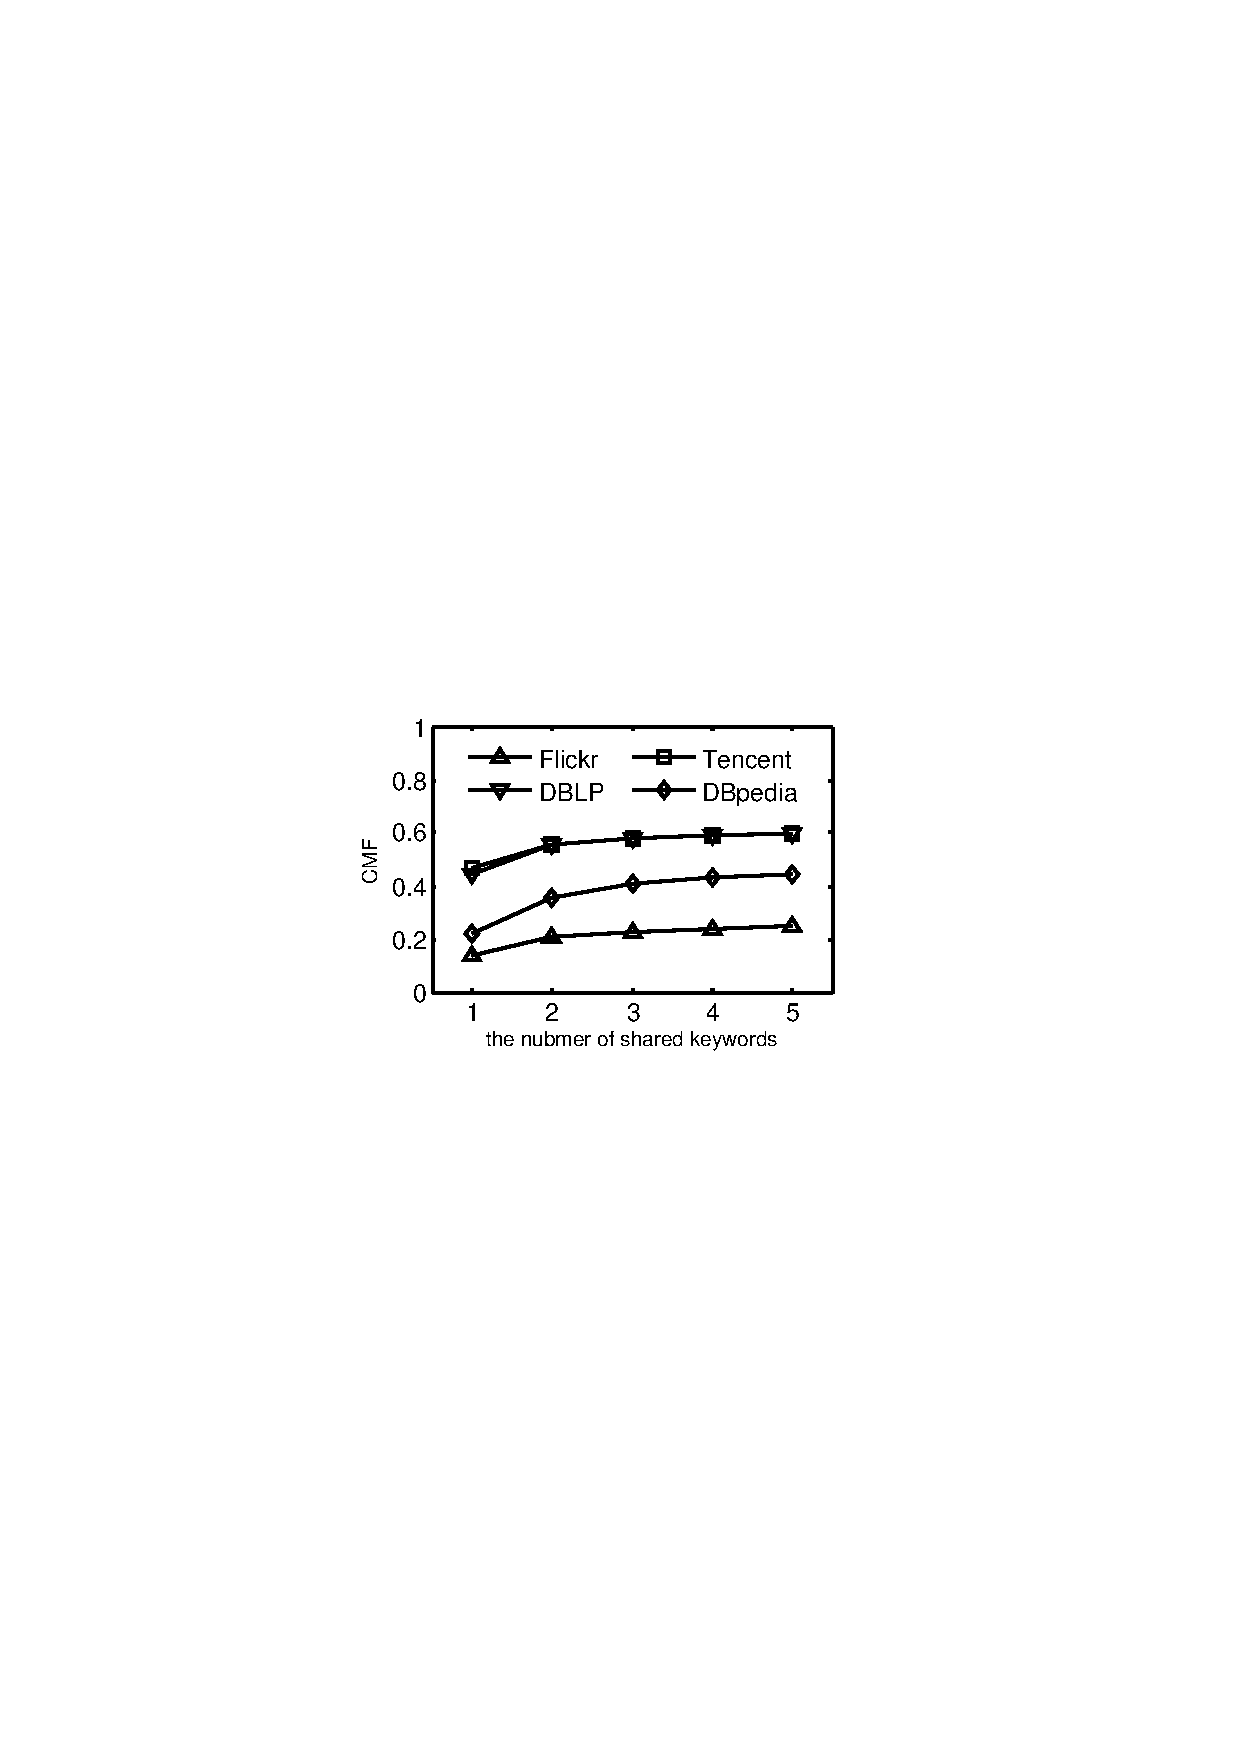
\includegraphics[width=.40\columnwidth]{figures/cmf-share}
            \label{fig:aqj}
        }
        \hspace{2ex}
        \subfigure[CPJ]{
            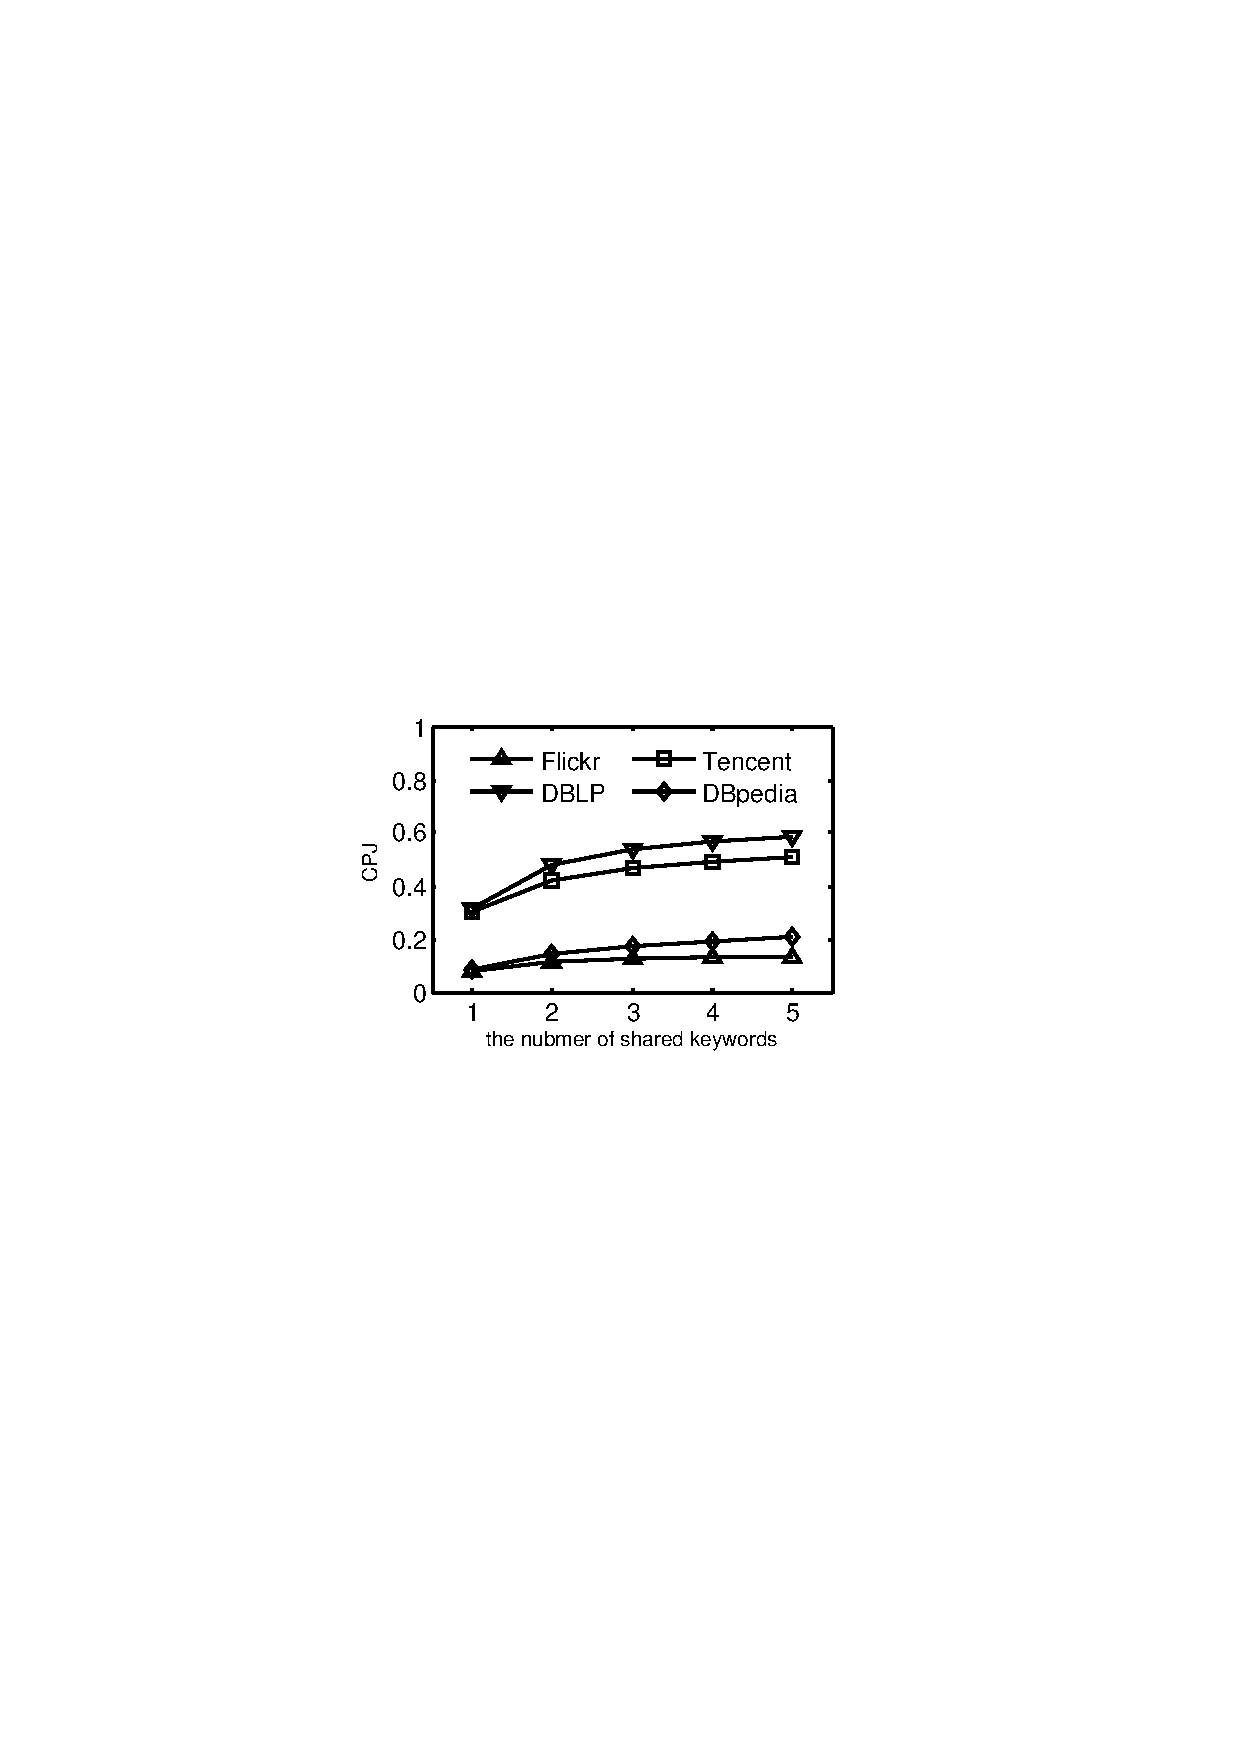
\includegraphics[width=.40\columnwidth]{figures/cpj-share}
            \label{fig:apj}
        }
    }
    \caption{AC-label length.}\label{fig:measure-share}
\end{figure}


{\bf 2. Comparison with existing CD methods}
As mentioned ahead, the existing CD methods for attributed graph can be adapted for community search. We choose to adapt {\tt CODICIL}~\cite{attr-www2013} for comparison. The main reasons are: (1) it has been tested on the ever reported largest attributed graph (vertex number:3.6M); (2) it identifies communities of comparable or superior quality than those of many existing methods like~\cite{attr-topic-kdd2008,attr-kdd2009}; and (3) it runs faster than many existing methods. Since {\tt CODICIL} needs users to specify the number of clusters expected, we set the numbers as 1K, 5K, 10K, 50K and 100K. The corresponding adapted algorithms are named as {\tt Cod1K}, $\cdots$, {\tt Cod100K} respectively. Other parameter settings are the same as those in~\cite{attr-www2013}. We first run these algorithms offline to obtain all the communities. Given a query vertex $q$, they return communities containing $q$ as the results.

We consider both keyword and structure for evaluating community quality.
(1) \emph{Keyword:} Figures~\ref{fig:detection-comp}(a) and (b) show that {\tt ACQ} (implemented by {\tt Dec}) always performs the best, in terms of CMF and CPJ.
(2) \emph{Structure:} As {\tt CODICIL} has no guarantee on vertices' minimum degrees, it is unfair to compare them using this metric. We intuitively compare their structure cohesiveness by reporting the average degree of the vertices in the communities and the percentage of vertices having degrees of 6 or more. When the number of clusters in {\tt CODICIL} is too large or too small, the structure cohesiveness becomes weak, as shown in Figures~\ref{fig:detection-comp}(c) and (d). {\tt ACQ} always performs better than {\tt CODICIL}, even when its number of cluster is well set (e.g., {\tt Cod10K} and {\tt Cod50K} on DBLP dataset).

\begin{figure}[]
\centering
    \begin{tabular}{c c}
        \begin{minipage}{3.36cm}
	        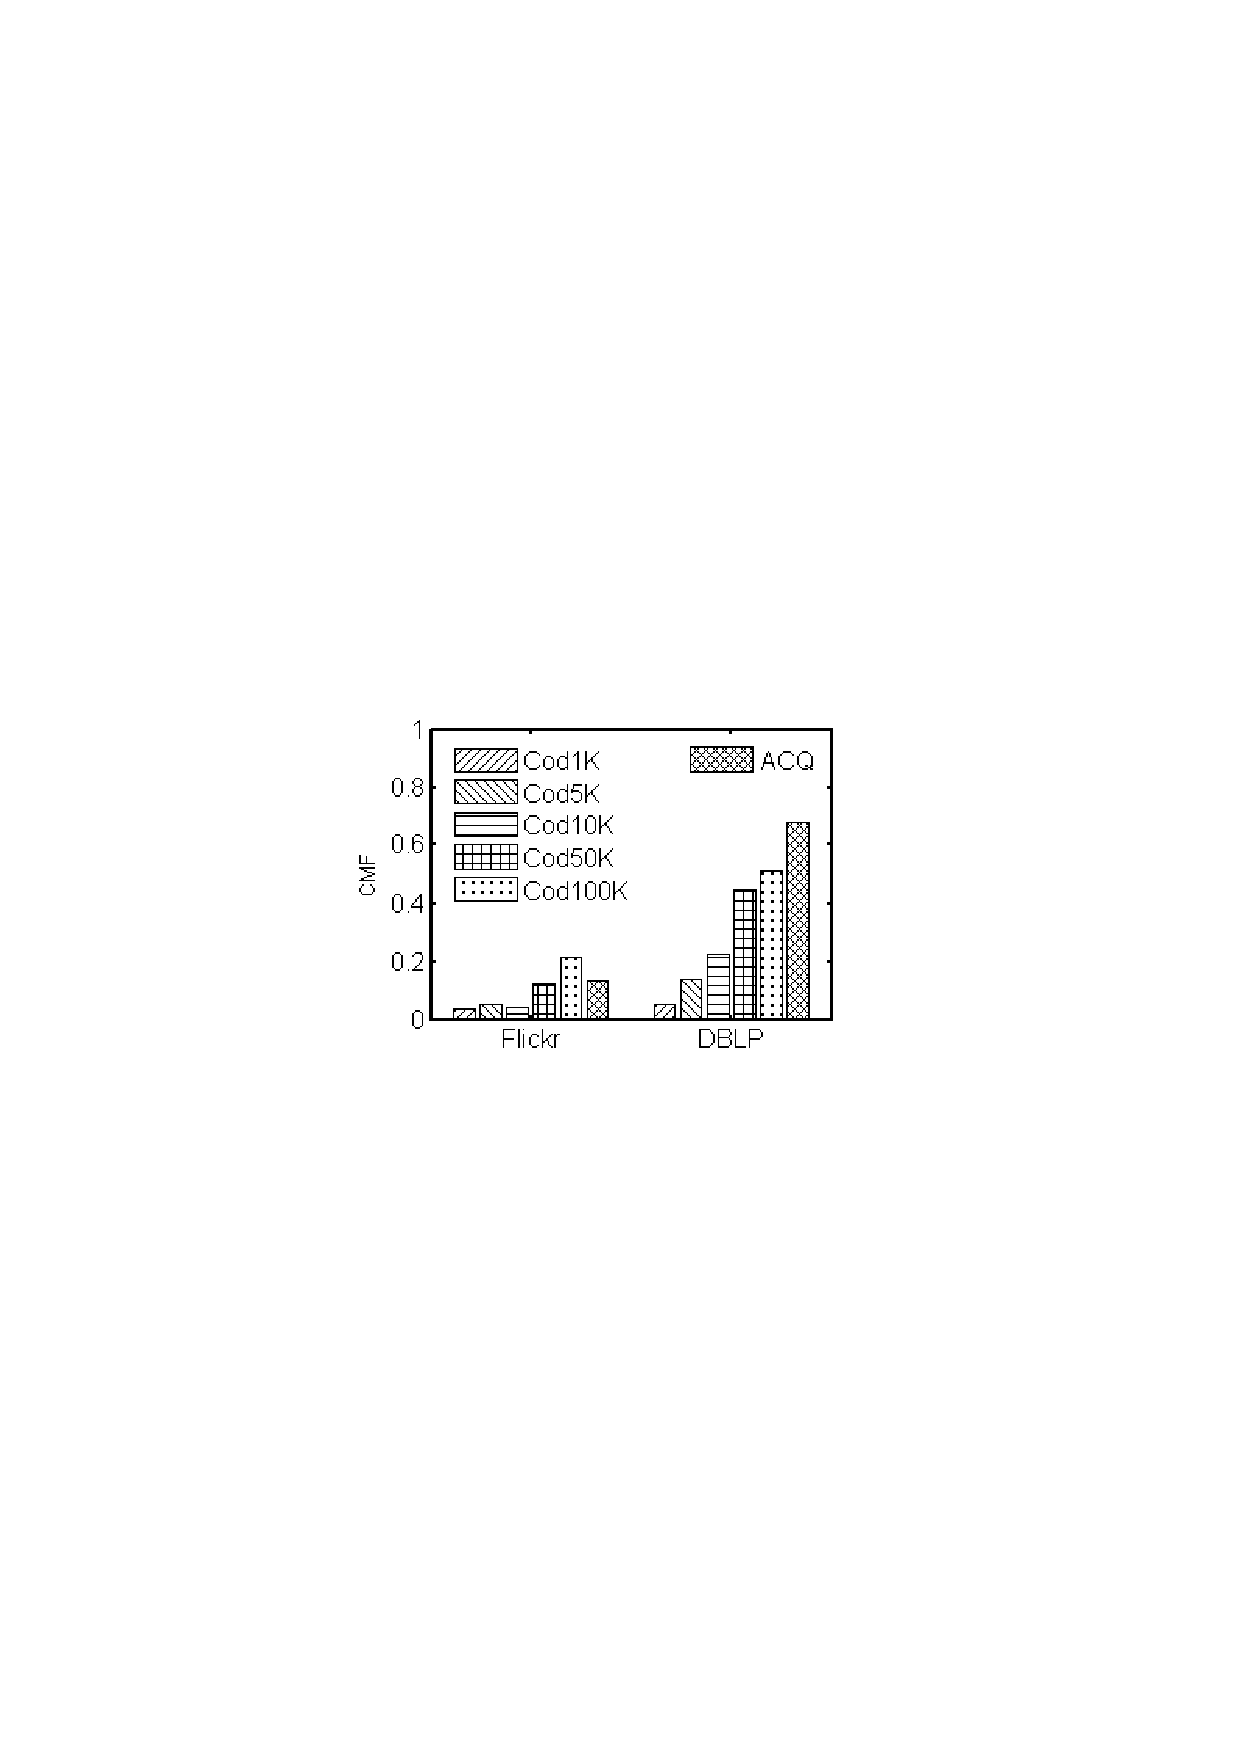
\includegraphics[width=3.35cm]{figures/cmfCOD}
        \end{minipage}
        &
        \begin{minipage}{3.36cm}
	     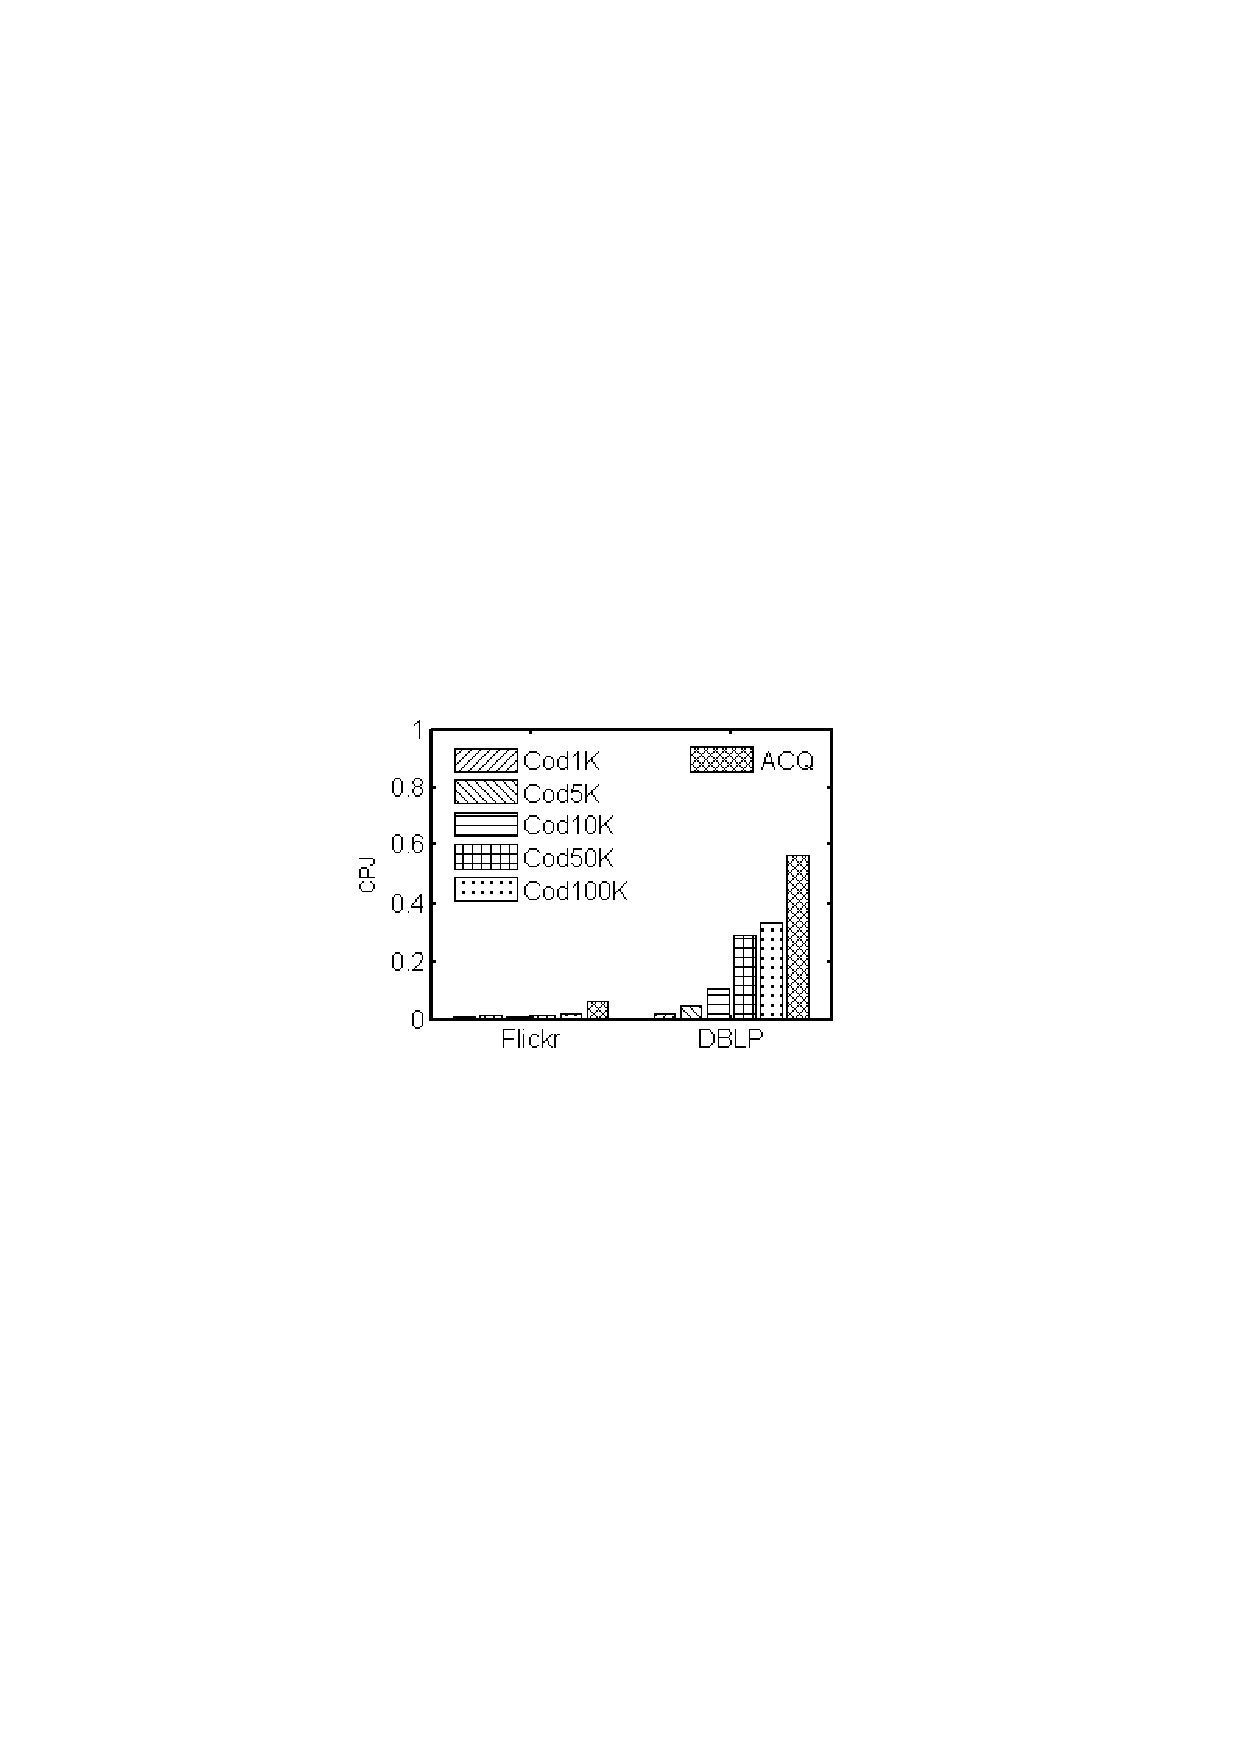
\includegraphics[width=3.35cm]{figures/cpjCOD}
         \end{minipage}
         \\
         \small (a) Keyword (CMF)
         &
         \small (b) Keyword (CPJ)
         \\

        \begin{minipage}{3.36cm}
	       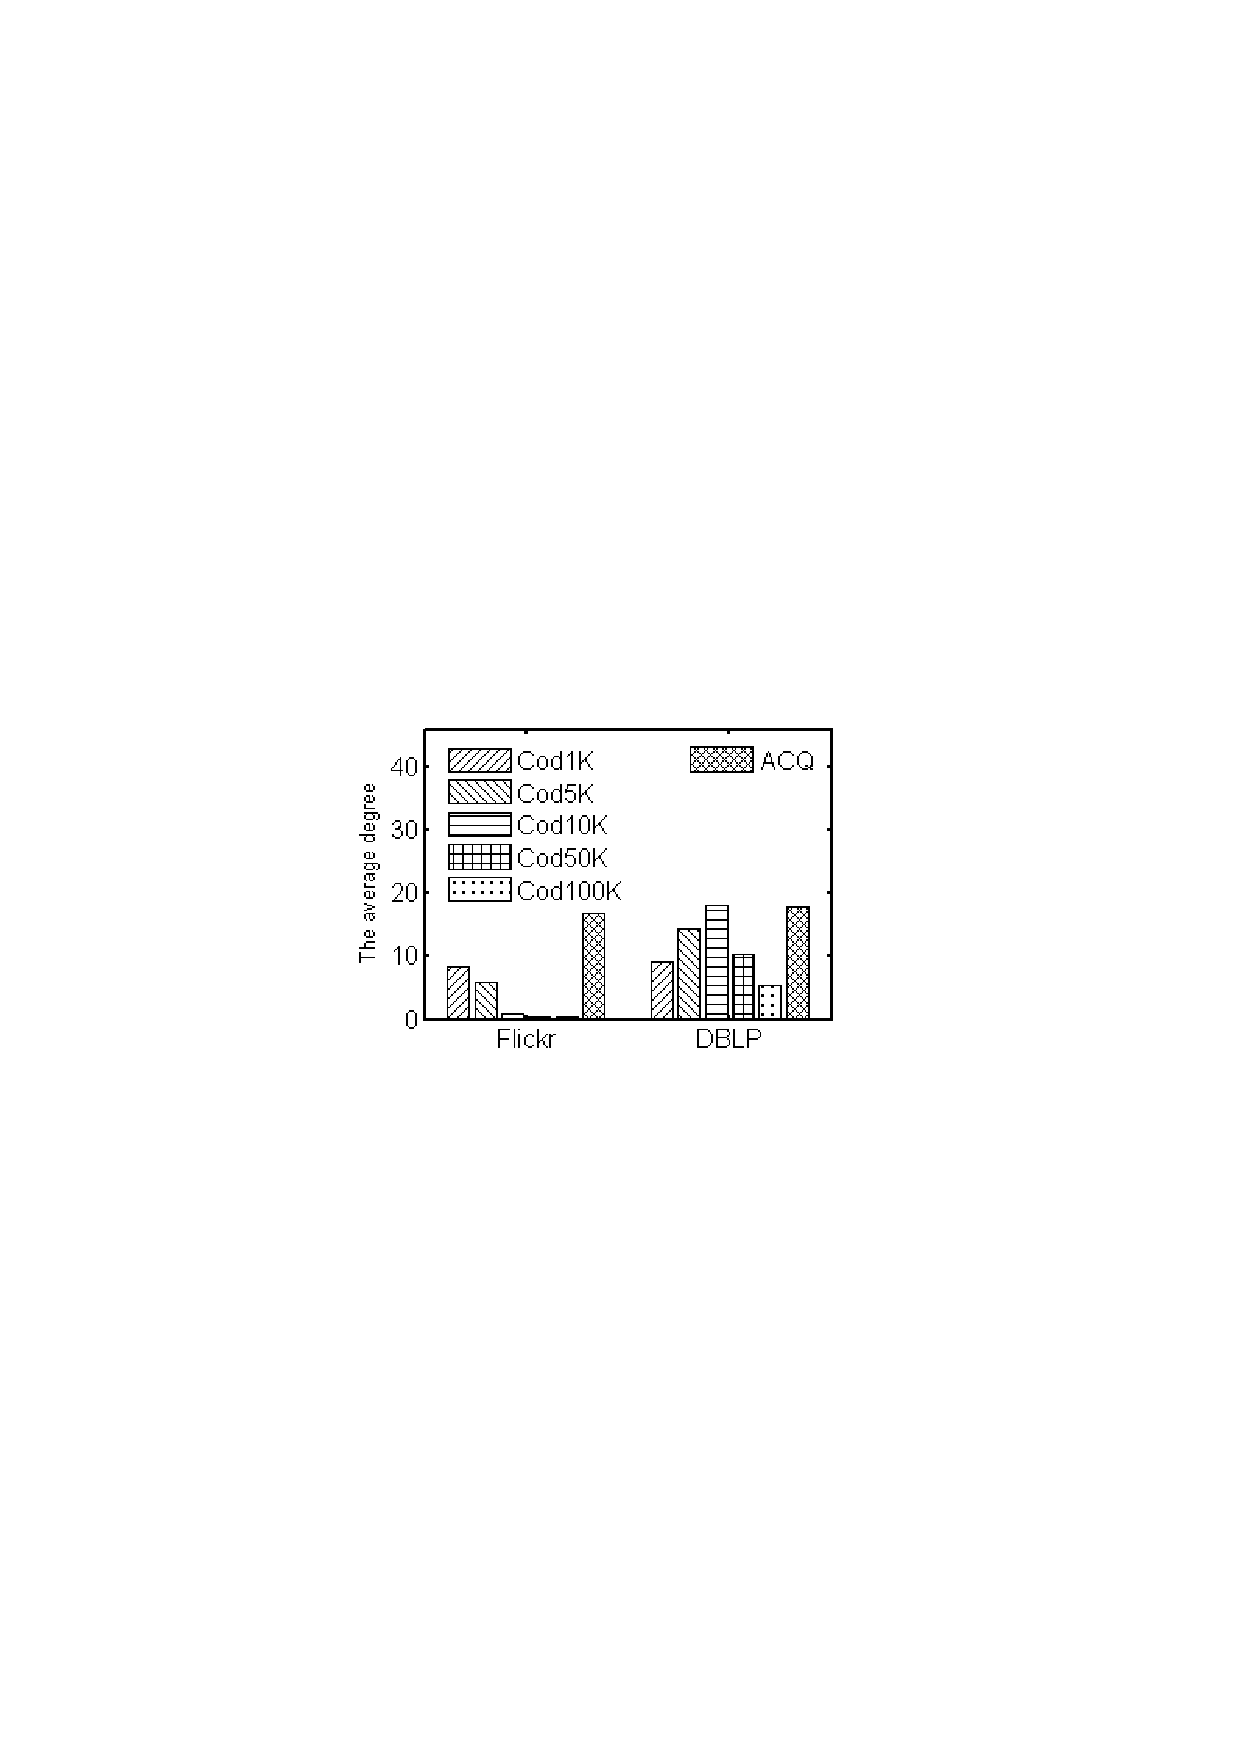
\includegraphics[width=3.35cm]{figures/avgDegCOD}
        \end{minipage}
        &
        \begin{minipage}{3.36cm}
	       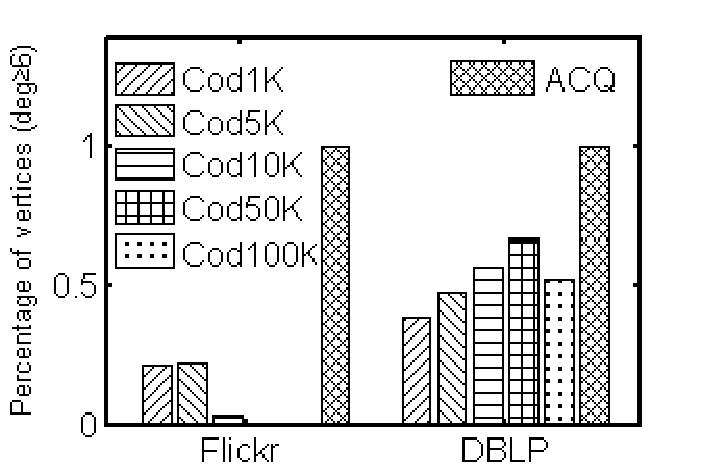
\includegraphics[width=3.35cm]{figures/deg6COD}
        \end{minipage}
        \\
        \small (c) Structure (Avg. degree)
        &
        \small (d) Structure (degree $\geq$ 6)
    \end{tabular}
    \caption{Comparing with community detection method.}
    \label{fig:detection-comp}
\end{figure}


{\bf 3. Comparison with existing CS methods.}
The existing methods mainly focus on non-attributed graphs. We implement two state-of-the-art methods:
{\tt Global}~\cite{KDD2010} and {\tt Local}~\cite{local2014}. Both of them use the metric minimum degree, we thus focus on the keyword cohesiveness. Figure~\ref{fig:search-comp} shows the CMF and CPJ values for the four datasets. We can see that the keyword cohesiveness of {\tt ACQ} is superior to both {\tt Global} and {\tt Local}, because {\tt ACQ} considers vertex keywords, while {\tt Global} and {\tt Local} do not.

\begin{figure}[ht]
    \centering
    \mbox{
        \subfigure[CMF]{
            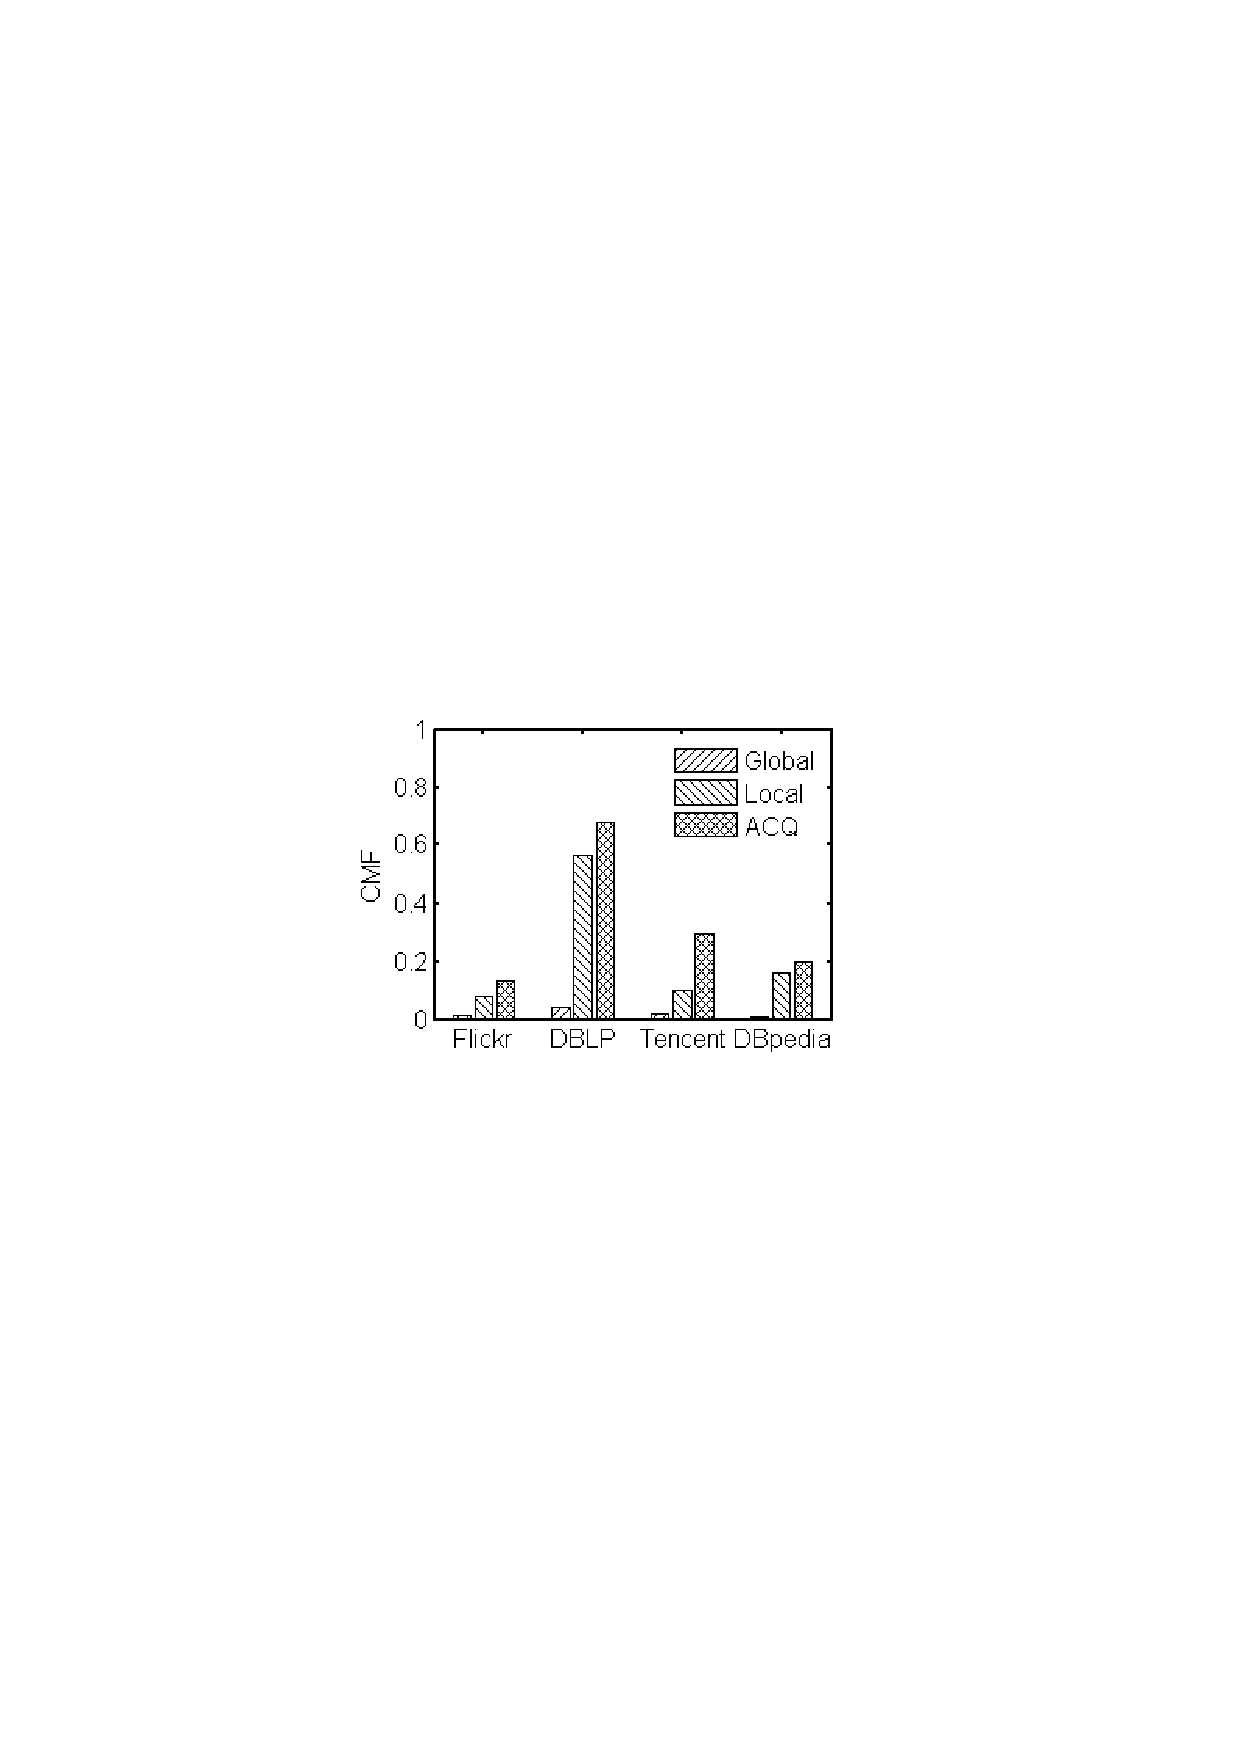
\includegraphics[width=.40\columnwidth]{figures/cmf}
            \label{fig:cmf}
        }
        \hspace{2ex}
        \subfigure[CPJ]{
            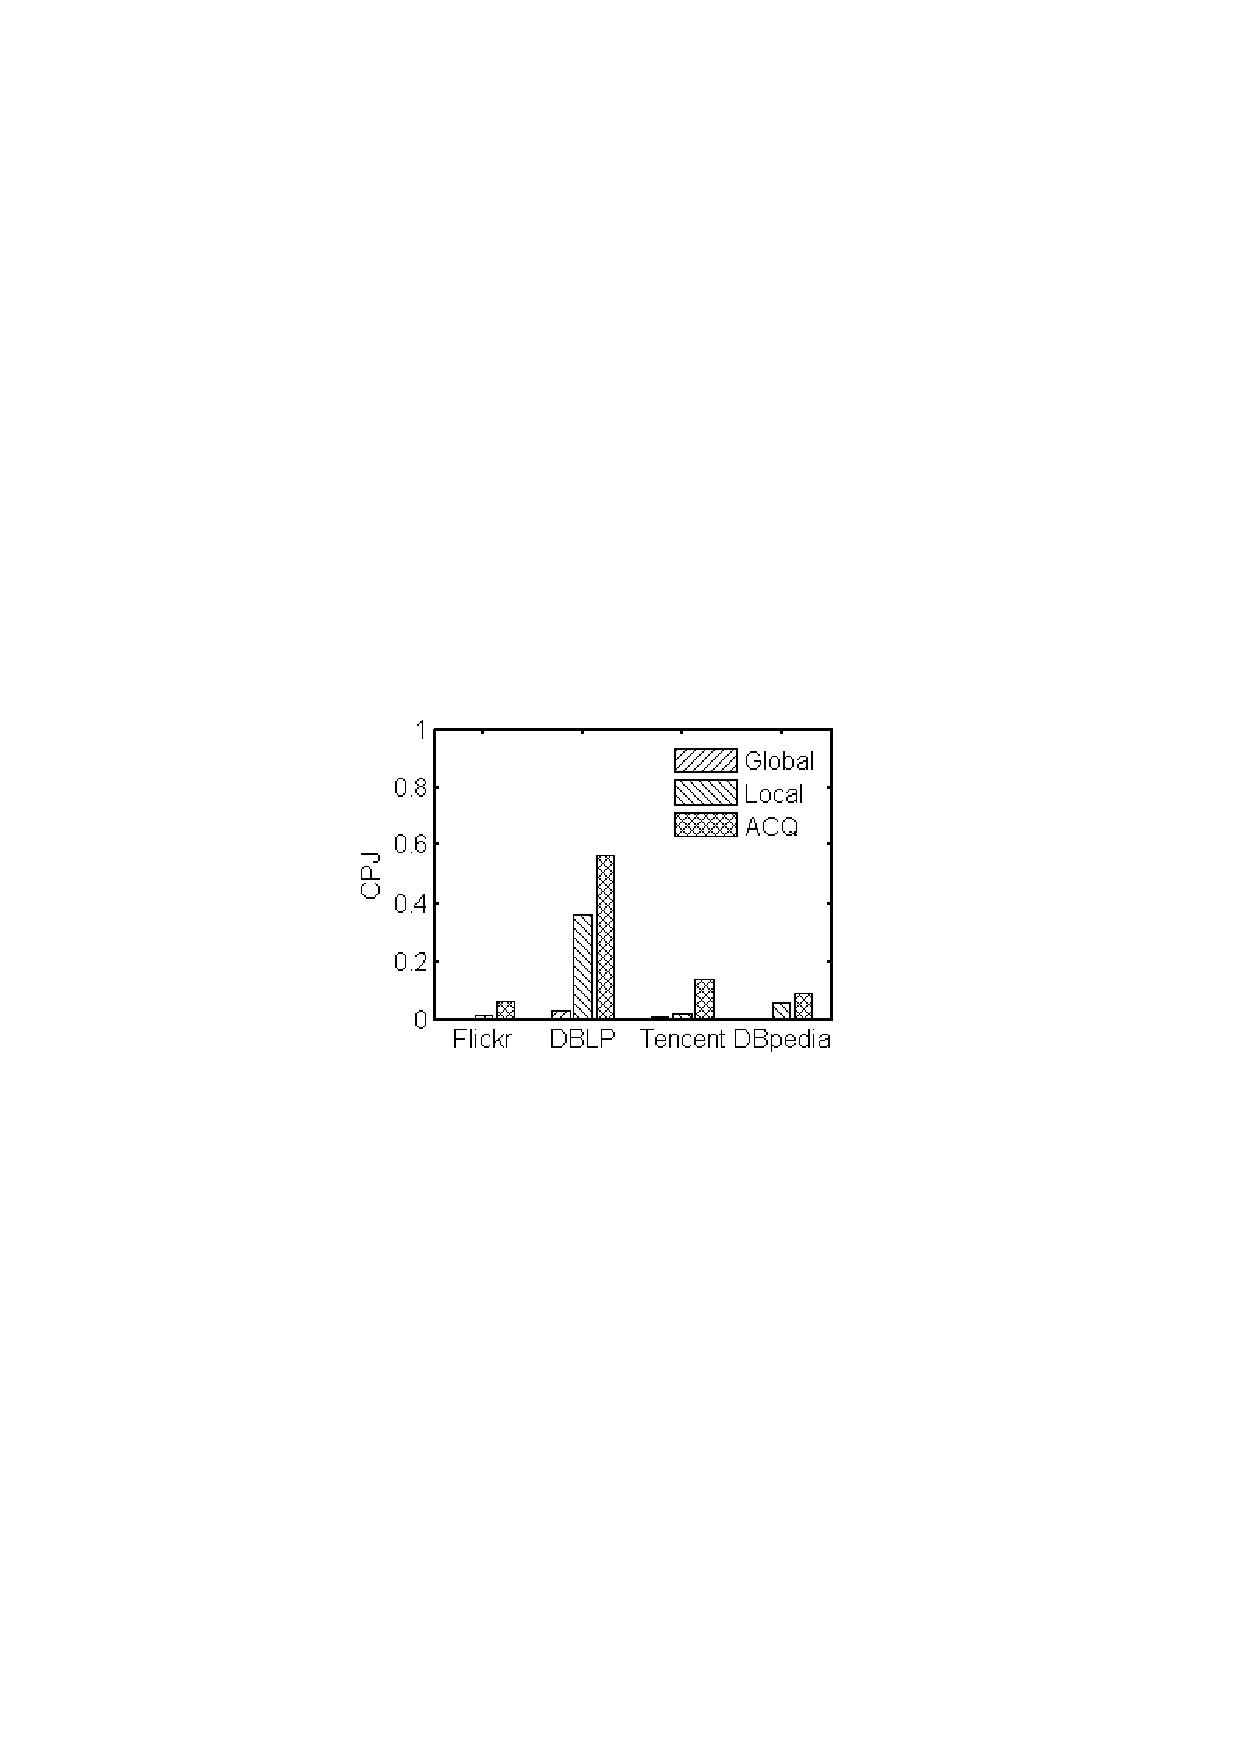
\includegraphics[width=.40\columnwidth]{figures/cpj}
            \label{fig:cpf}
        }
    }
    \caption{Comparing with community search methods.}
    \label{fig:search-comp}
\end{figure}

\subsubsection{A Case Study}
\label{caseStudy}

We next perform a case study on the DBLP dataset, in which we consider two renowned researchers in database and data mining: Jim Gray and Jiawei Han. We use $k=4$ here. We use {\tt Cod50K} to represent {\tt CODICIL} for further analysis.
We mainly consider the input query keyword set $S$, keywords and sizes of communities.

{\bf 1. Effect of $S$.} Figure~\ref{fig:jiawei} shows two ACs of Jiawei (AC-labels are shown in the captions),
where the query keyword set $S$ are set as $\{$analysis, mine, data, information, network$\}$ and $\{$mine, data, pattern, database$\}$ respectively. These two groups of Jiawei's collaborators are involved in graph analysis (Figure~\ref{fig:jiawei1}) and pattern mining (Figure~\ref{fig:jiawei2}). Although these researchers all have close co-author relationship with Jiawei, the use of the input keyword set $S$ enables the identification of communities with different research themes.
For Jim, we can obtain similar results as discussed in Section~\ref{intro} (Figure~\ref{fig:jim}).
While for {\tt CODICIL}, it is not clear how to consider the keyword set $S$, and we thus do not show the results.

\begin{figure}[ht]
    \centering
    \mbox{
        \subfigure[$\{$analysis, data, information, network$\}$]{
            
\includegraphics[width=.40\columnwidth]{figures/jiawei1}
            \label{fig:jiawei1}
        }
        \hspace{2ex}
        \subfigure[$\{$mine, data, pattern, database$\}$]{
            
\includegraphics[width=.40\columnwidth]{figures/jiawei2}
            \label{fig:jiawei2}
        }
    }
    \caption{Jiawei Han's ACs.}
    \label{fig:jiawei}
\end{figure}

\begin{figure}[h]
    \centering
    \mbox{
        \subfigure[Jim Gray]{
            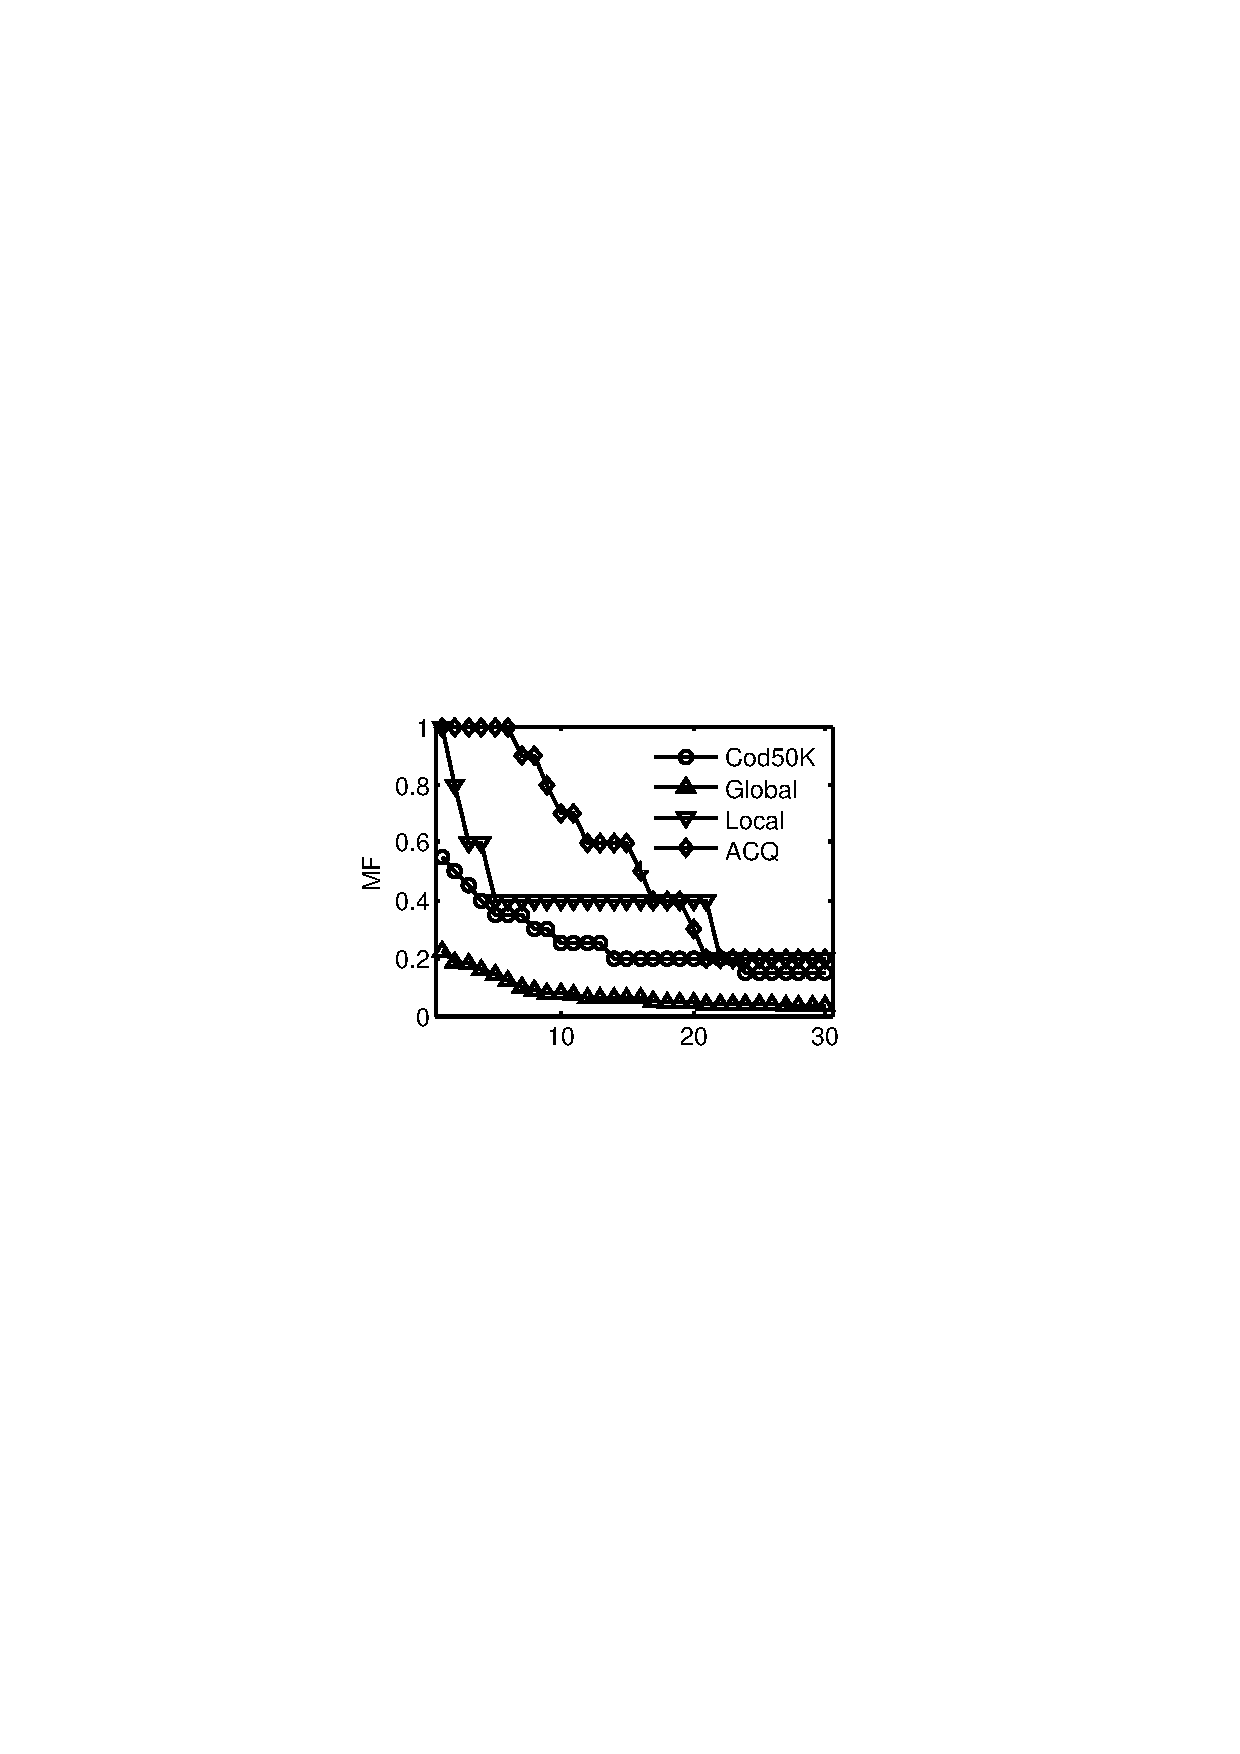
\includegraphics[width=.40\columnwidth]{figures/jim-mf}
            \label{fig:jimFreq30}
        }
        \hspace{2ex}
        \subfigure[Jiawei Han]{
            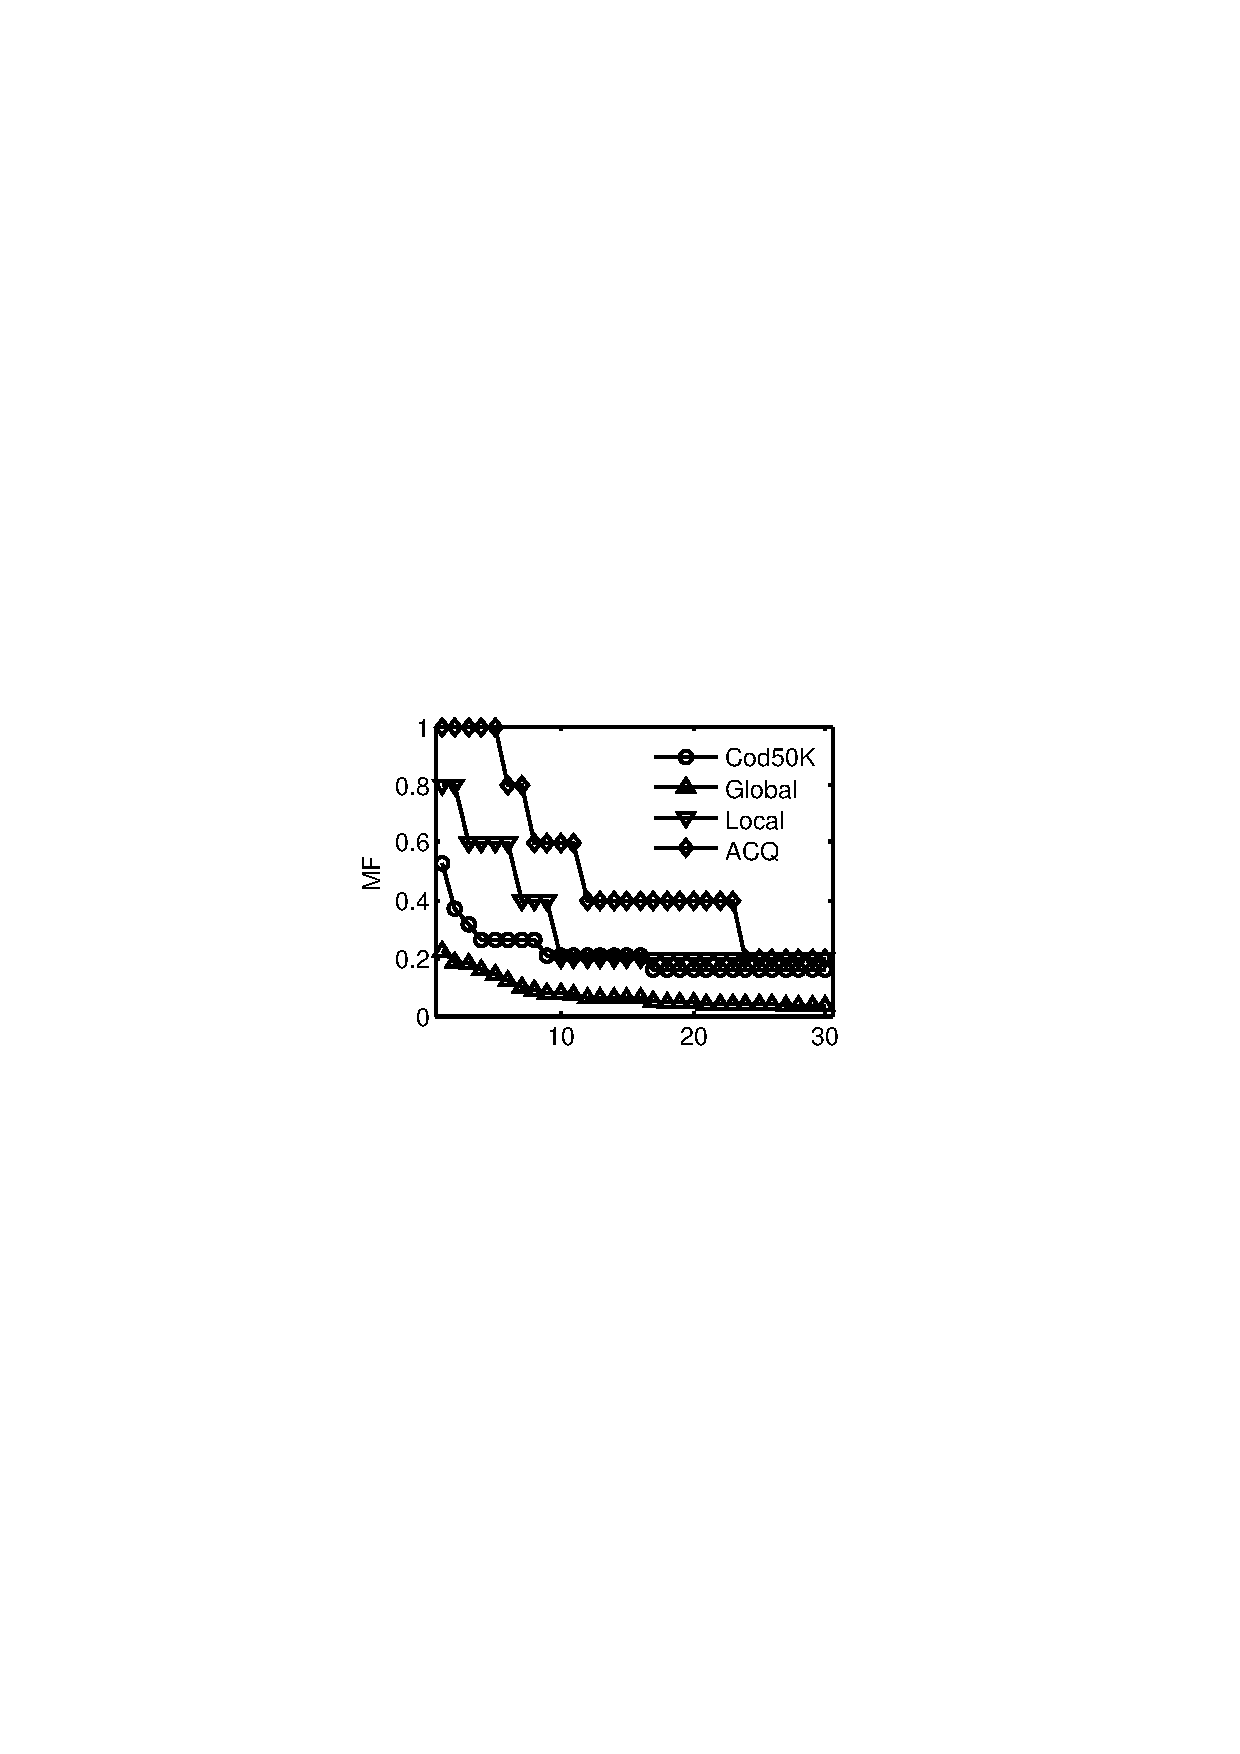
\includegraphics[width=.40\columnwidth]{figures/jiawei-mf}
            \label{fig:jiaweiFreq30}
        }
    }
    \caption{Frequency distribution of keywords.}\label{fig:freq50}
\end{figure}

\vspace{-0.2cm}
\begin{table}[h]
  \centering \footnotesize \caption {\# distinct keywords of communities.}
  \label{tab:kws}
  \begin{tabular}{c|c|c|c|c}
     \hline
          \bf{Researcher}            & {\tt Cod50K} &  \bf{{\tt Global}} & {\tt Local} & {\tt ACQ}\\
     \hline\hline
          Jim Gray   &     134       & 139,881      &     60     &    44    \\
     \hline
          Jiawei Han &     140       & 139,881      &     58     &    54\\
     \hline
  \end{tabular}
\end{table}

{\bf 2. Keyword analysis.} We analyze the frequency distribution of keywords in their communities.
Specifically, given a keyword $w_h$, we define the member frequency (MF) of $w_h$ as:
$MF({w_h}, C(q)) = \frac{1}{\mathcal{L}}\sum\limits_{i = 1}^\mathcal{L} {\frac{{{f_{i,h}}}}{{\left| {{C_i}} \right|}}}$.
The MF measures the occurrence of a keyword in $C(q)$. For each $C_q$ generated by an algorithm, we select 30 keywords with the highest MF values. We report the MF of each keyword in descending order of their MF values in Figure~\ref{fig:freq50}.
We see that {\tt ACQ} has the highest MF values for the top 20 keywords. Thus, the keywords associated with the communities generated by {\tt ACQ} tend to repeat among the community members.

The number of distinct keywords of {\tt ACQ} communities is also the fewest, as shown in Table~\ref{tab:kws}.
For example, the $k$-$\widehat{core}$ returned by {\tt Global} has over $139K$ distinct keywords,
about 2,300 times more than that returned by {\tt ACQ} (less than 60 keywords). While the semantics of the $k$-$\widehat{core}$ can be difficult to understand, the small number of distinct keywords of AC makes it easier to understand why the community is so formed. We further report the keywords with the 6 highest MF values in Jim and Jiawei's communities in Tables~\ref{tab:jim} and~\ref{tab:jiawei}. We can see that, words ``sloan'',  ``digital'', ``sky'', ``survey'', and ``sdss'' reflect that the community is likely about the SDSS project led by Jim. The top-6 keywords of Jiawei's AC are related to heterogenous networks. In contrast, the keywords of {\tt Global} and {\tt Local} tend to be less related to the query keyword set, and thus they cannot be used to characterize the communities specifically related to Jiawei.
Note that the top-6 keywords of {\tt Global} are the same for both Jim and Jiawei, as they are in the same $k$-$\widehat{core}$.
The overall results show that, {\tt ACQ} performs better than other methods.

\begin{table}[htp]
  \centering \footnotesize \caption {Top-6 keywords (Jim Gray).}
  \label{tab:jim}
  \begin{tabular}{c|l}
     \hline
          \bf{Algo.}   & \multicolumn{1}{c}{\textbf{Keywords}}\\
     \hline\hline
          {\tt Cod50K} & server, archive, sloan, digital, database\\
     \hline
          {\tt Global} & use, system, model, network, analysis, data\\
     \hline
          {\tt Local}  & database, system, multipetabyte, data, lsst, story\\
     \hline
          {\tt ACQ}    & sloan, digital, sky, data, sdss, server\\
     \hline
  \end{tabular}
\end{table}

\begin{table}[htp]
  \centering \footnotesize \caption {Top-6 keywords (Jiawei Han).}
  \label{tab:jiawei}
  \begin{tabular}{c|l}
     \hline
          \bf{Algo.}   & \multicolumn{1}{c}{\textbf{Keywords}}\\
     \hline\hline
          {\tt Cod50K} & information, mine, data, cube, text, network\\
     \hline
          {\tt Global} & use, system, model, network, analysis, data\\
     \hline
          {\tt Local}  & scalable, topical, text, phrase, corpus, mine\\
     \hline
          {\tt ACQ}    & mine, analysis, data, information, network, heterog\\
     \hline
  \end{tabular}
\end{table}



\textbf{3. Effect of $k$ on community size.}  We vary the value of $k$ and report the average size of communities in Figure~\ref{fig:size}. We can see that  the communities returned by {\tt Global} are extremely large (more than $10^5$), which can make them difficult for a query user to analyze. The community size of {\tt Local} increases sharply when $k$=8. In this situation, {\tt Local} returns the same community as {\tt Global}. The size of an AC is relatively insensitive to the change of $k$, as AC contains around a hundred vertices for a wide range of values of $k$.

\begin{figure}[ht]
    \centering
    \mbox{
        \subfigure[Jim Gray]{
            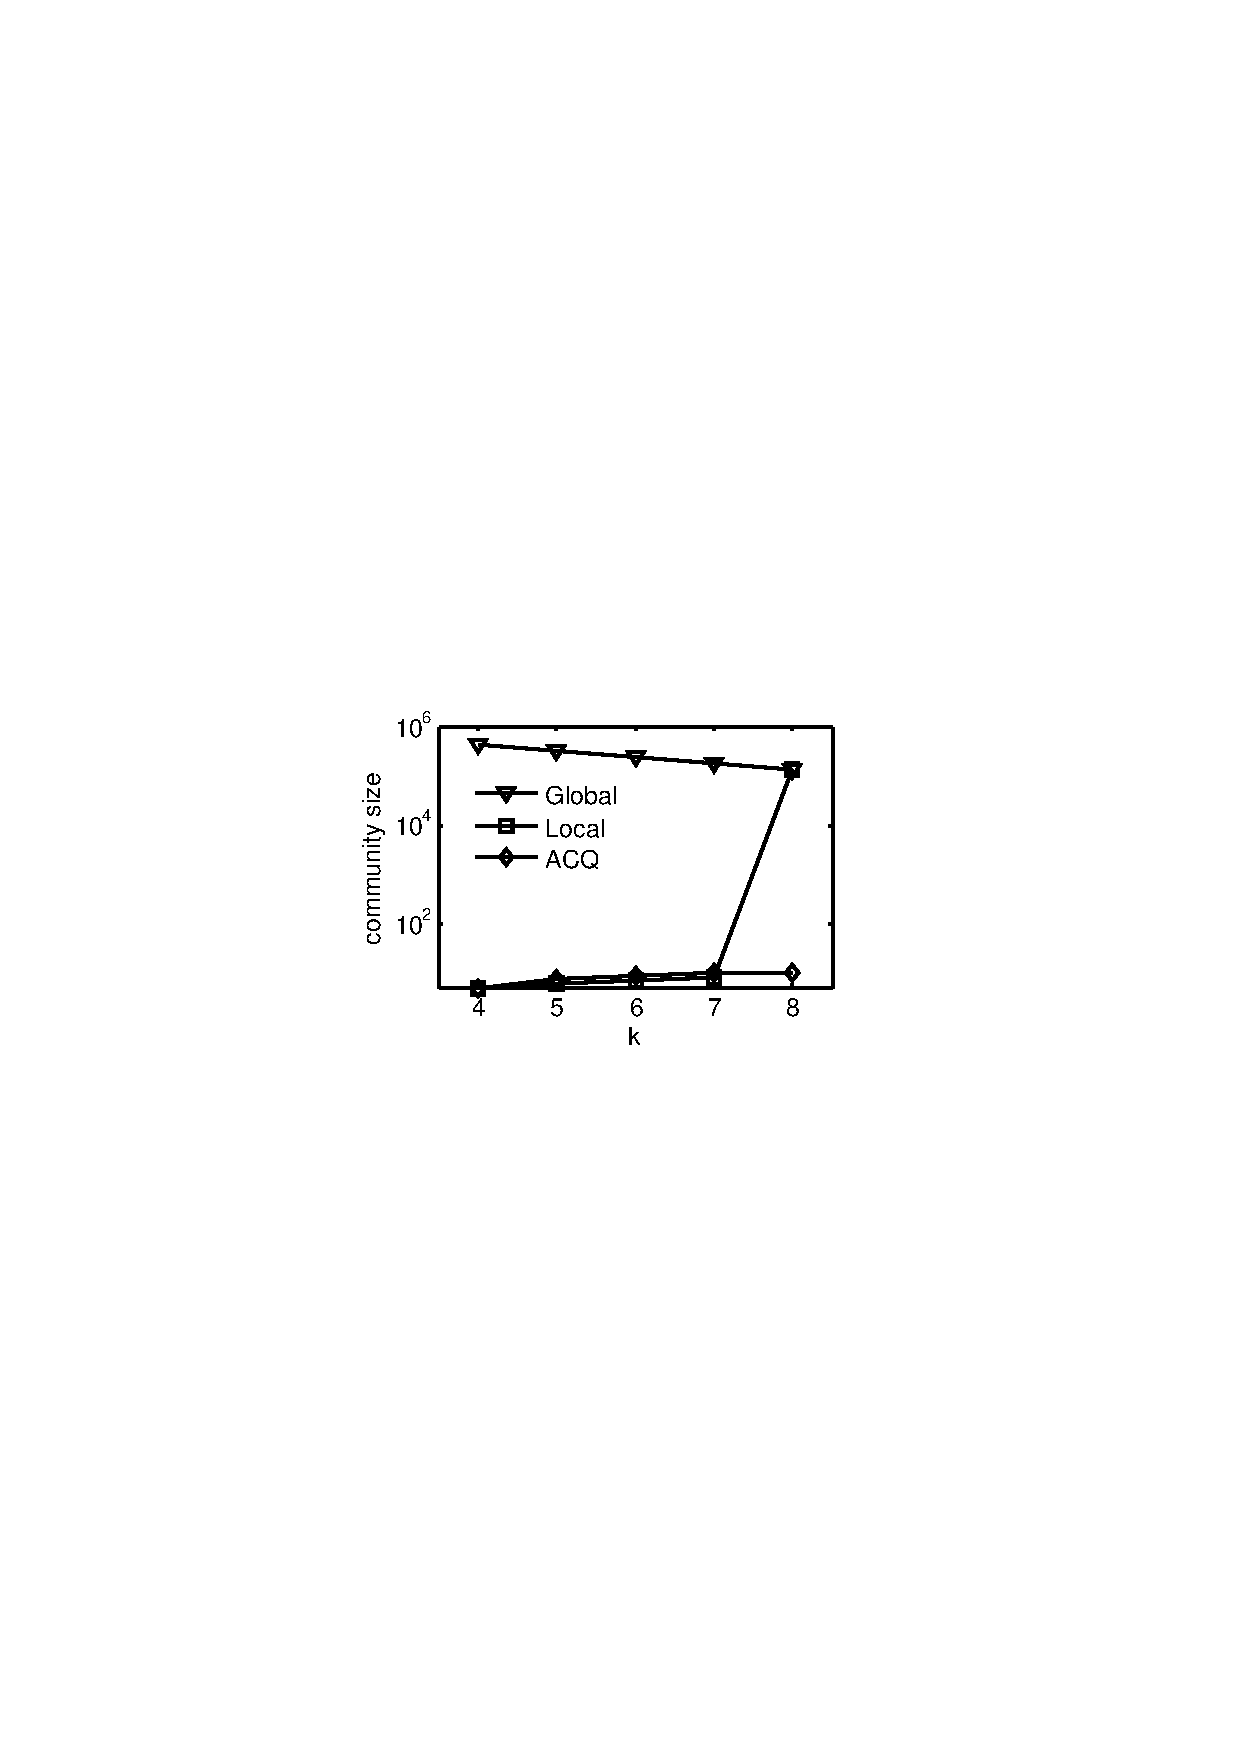
\includegraphics[width=.40\columnwidth]{figures/jim-size}
            \label{fig:jimSize}
        }
        \hspace{2ex}
        \subfigure[Jiawei Han]{
            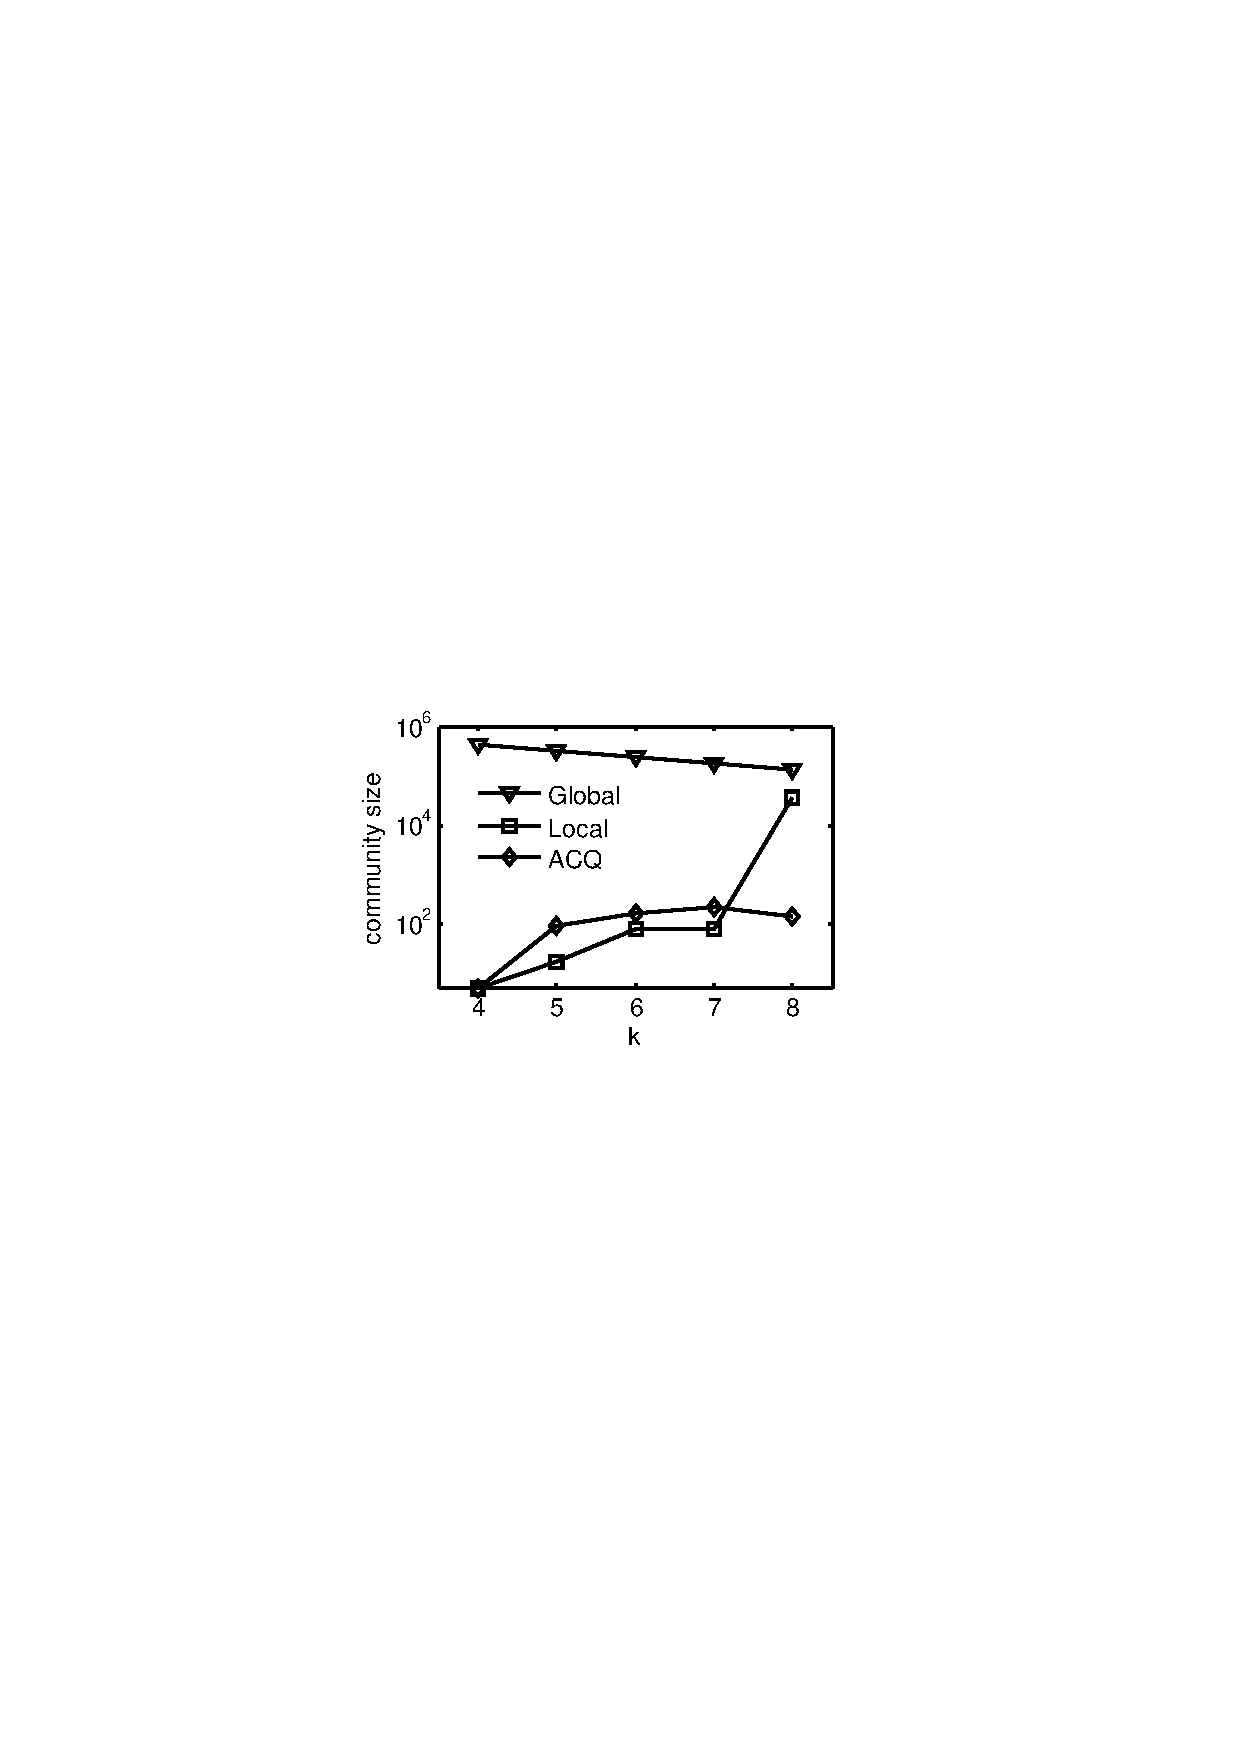
\includegraphics[width=.40\columnwidth]{figures/jiawei-size}
            \label{fig:jiaweiSize}
        }
    }
    \caption{Community size.}
    \label{fig:size}
\end{figure}




\subsection{Results on Efficiency}
\label{efficiency}

\begin{figure*}[htp]
\hspace*{-.4cm}
\centering
\begin{tabular}{c c c c}
  \begin{minipage}{3.76cm}
	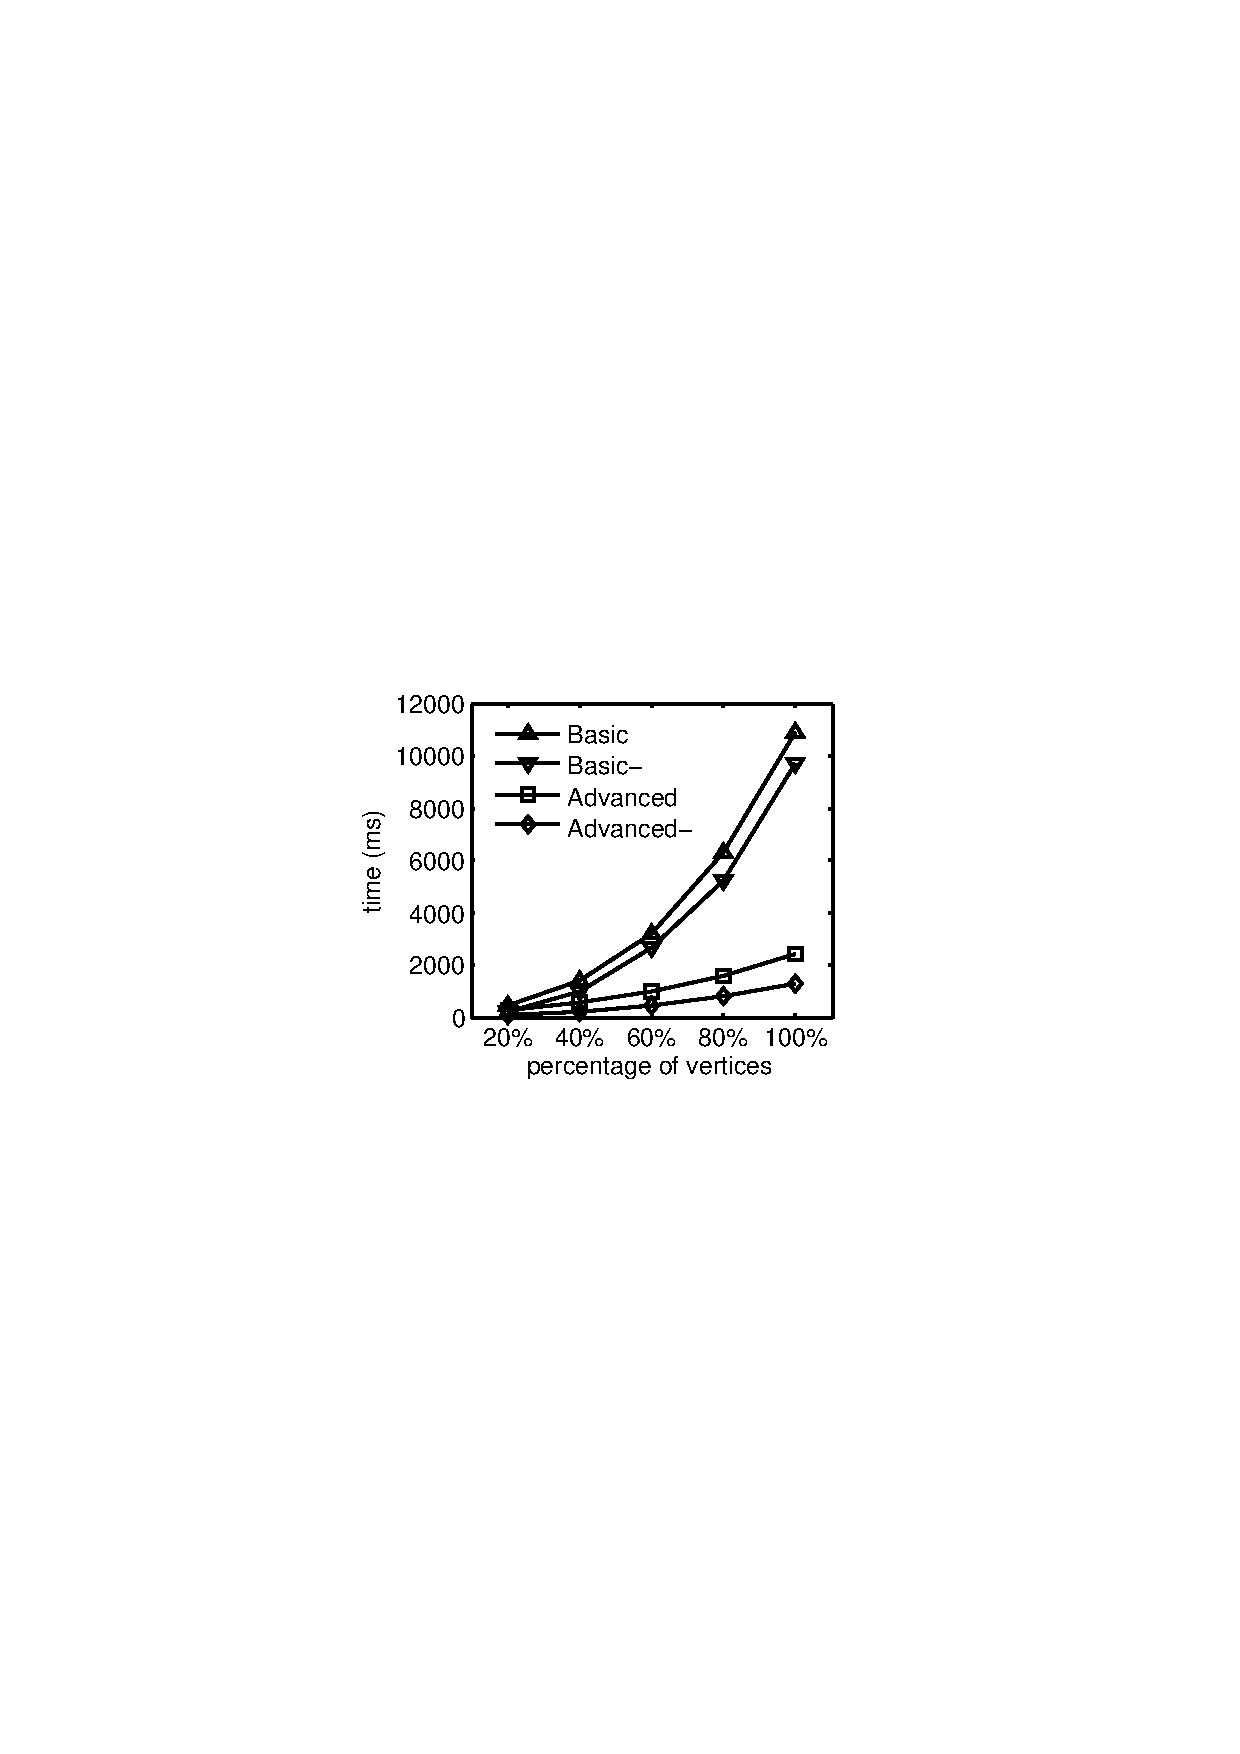
\includegraphics[width=3.725cm]{figures/flickr-index}
  \end{minipage}
  &
  \begin{minipage}{3.76cm}
	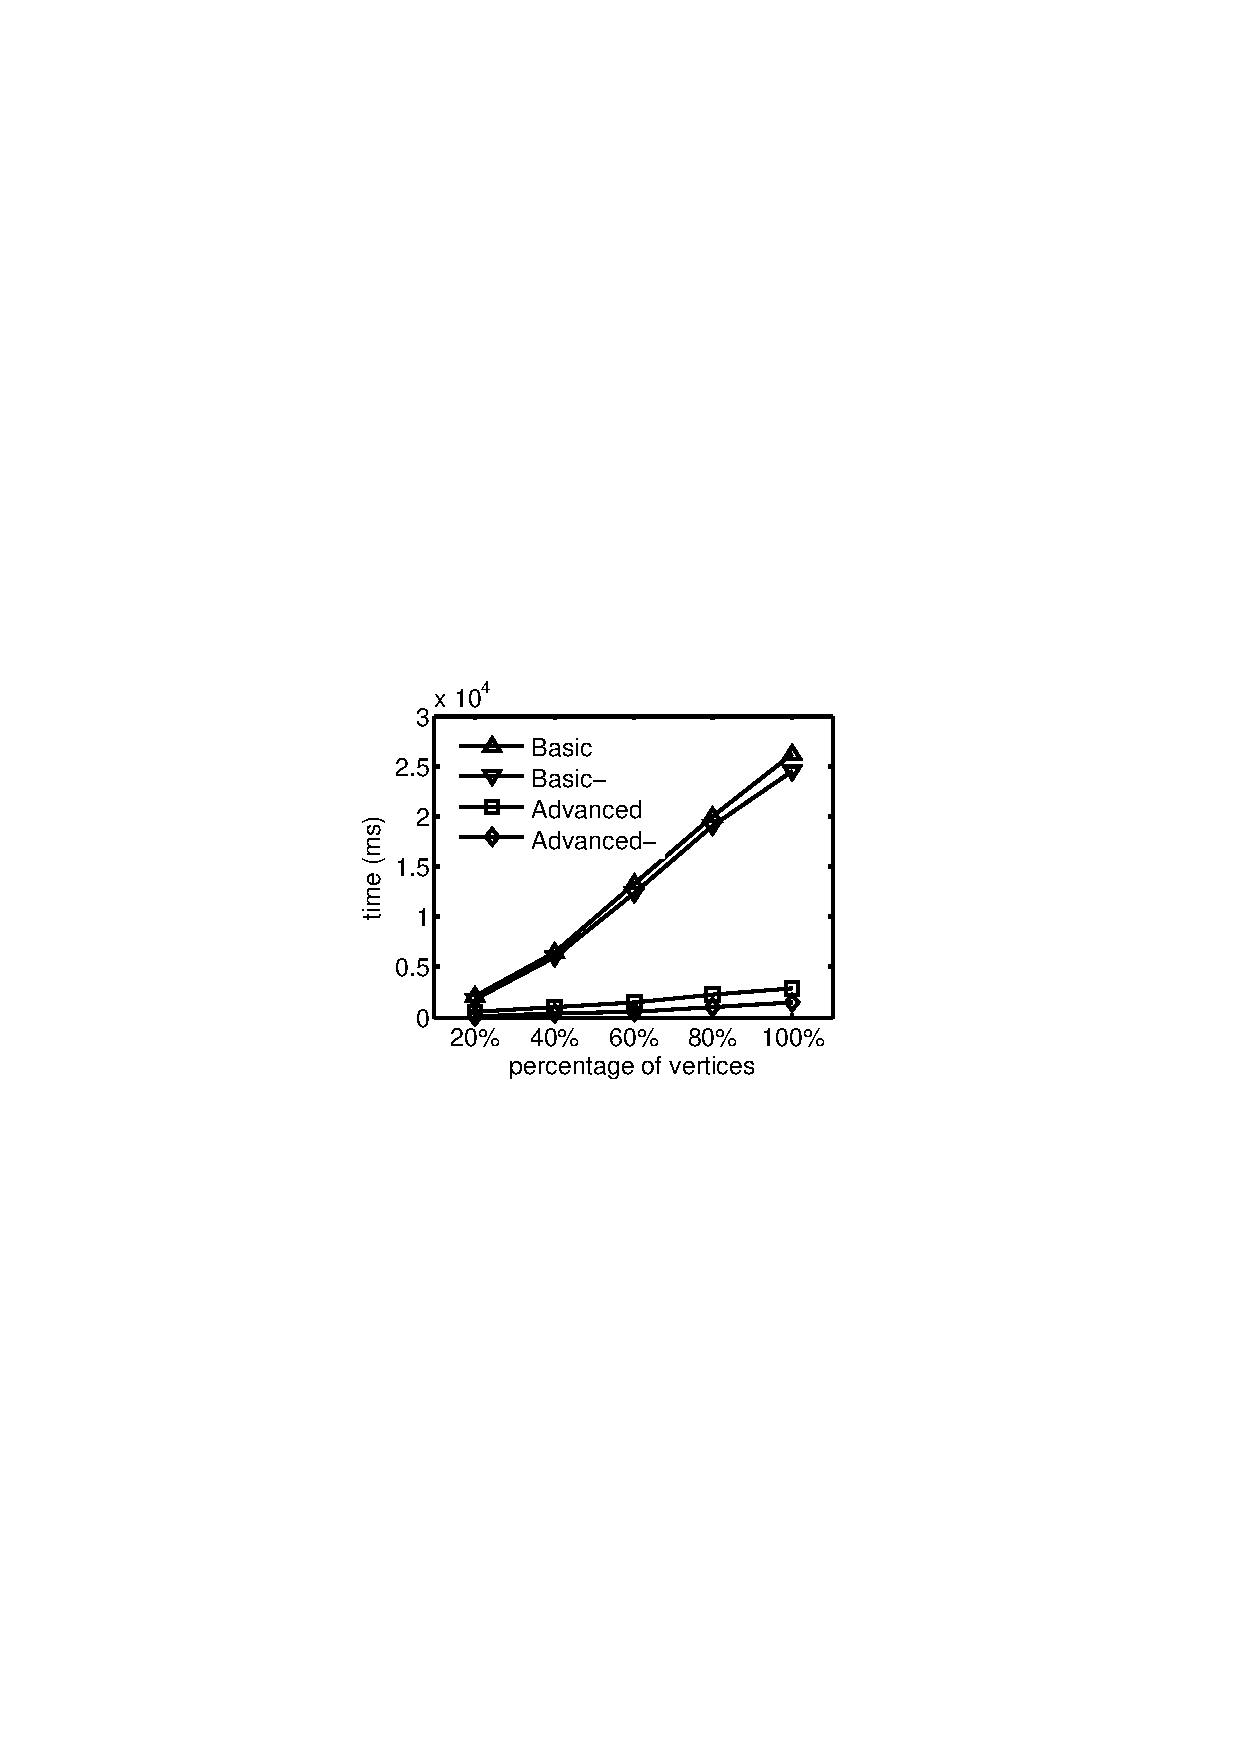
\includegraphics[width=3.725cm]{figures/dblp-index}
  \end{minipage}
  &
  \begin{minipage}{3.76cm}
	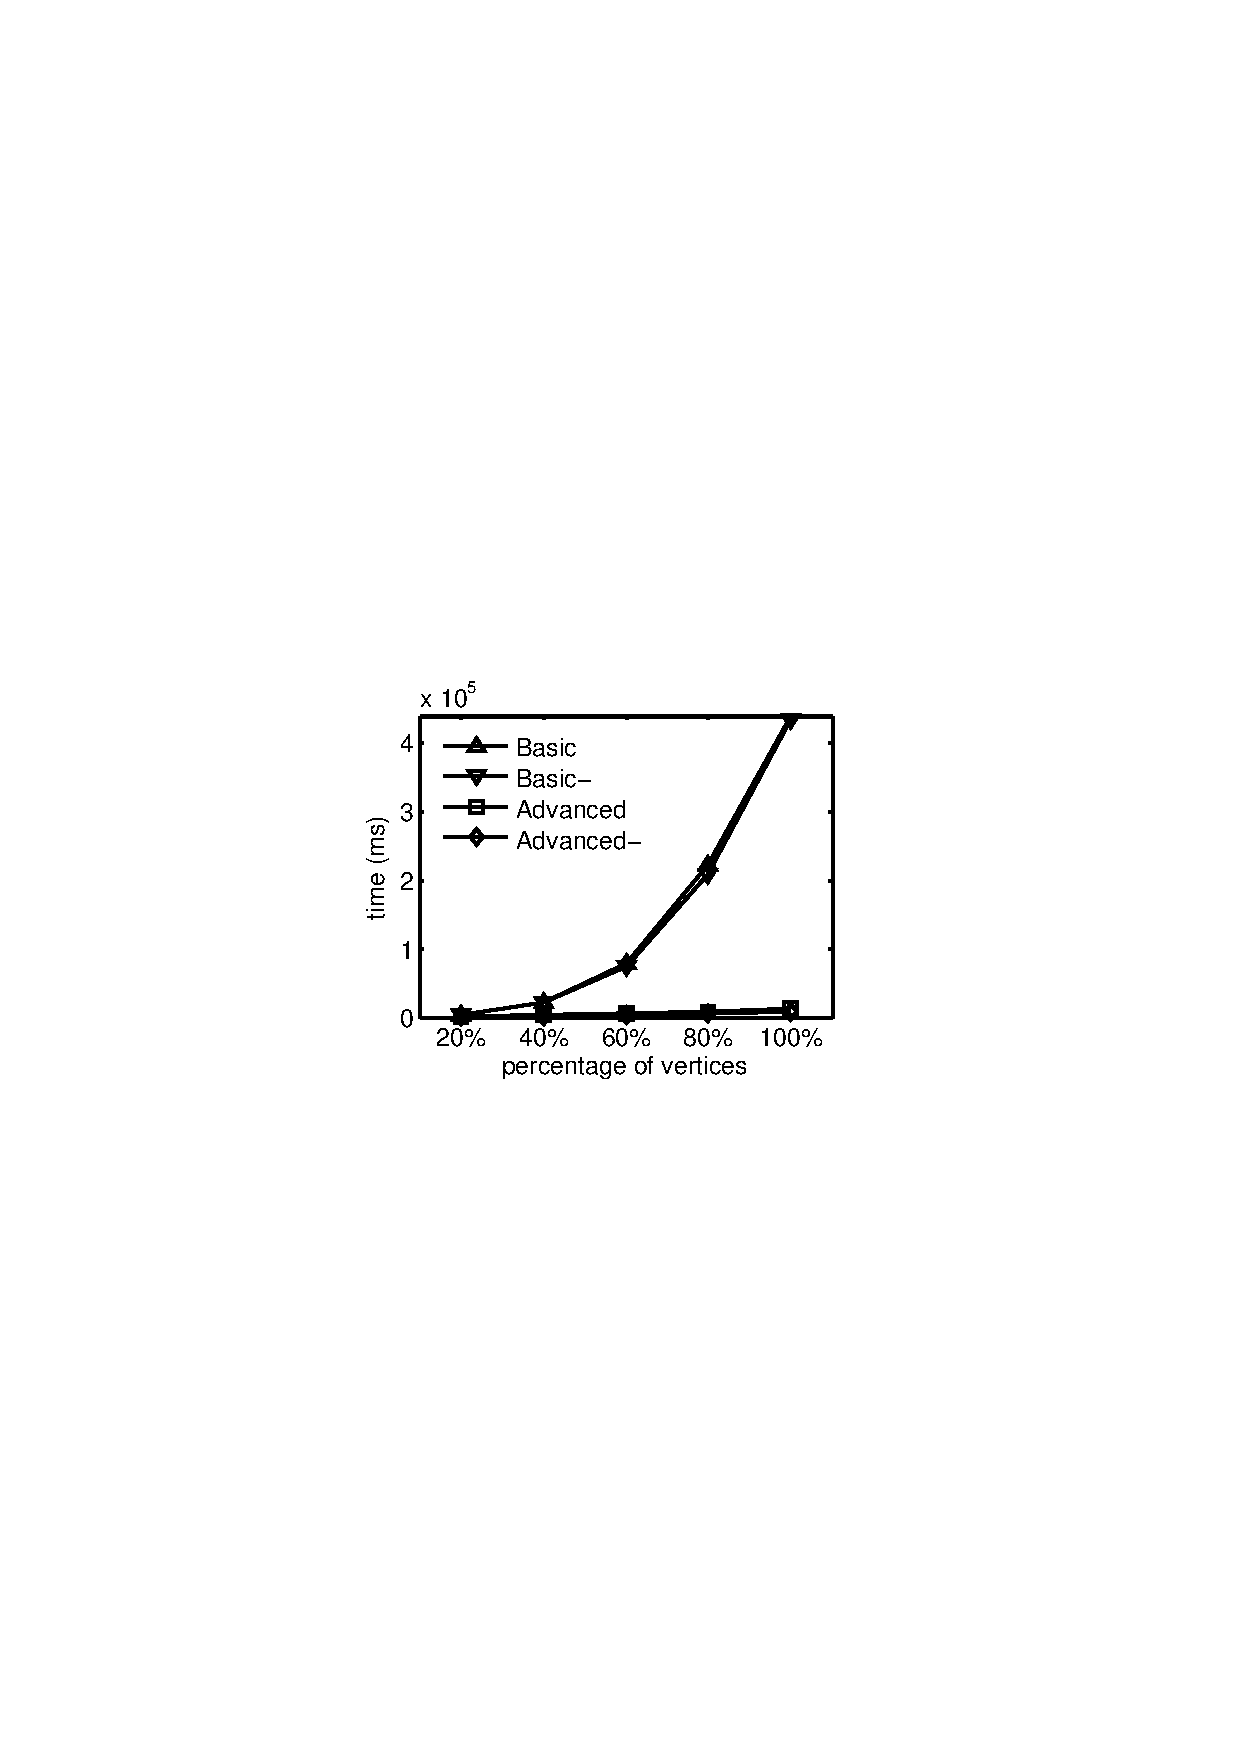
\includegraphics[width=3.725cm]{figures/tencent-index}
  \end{minipage}
  &
  \begin{minipage}{3.76cm}
	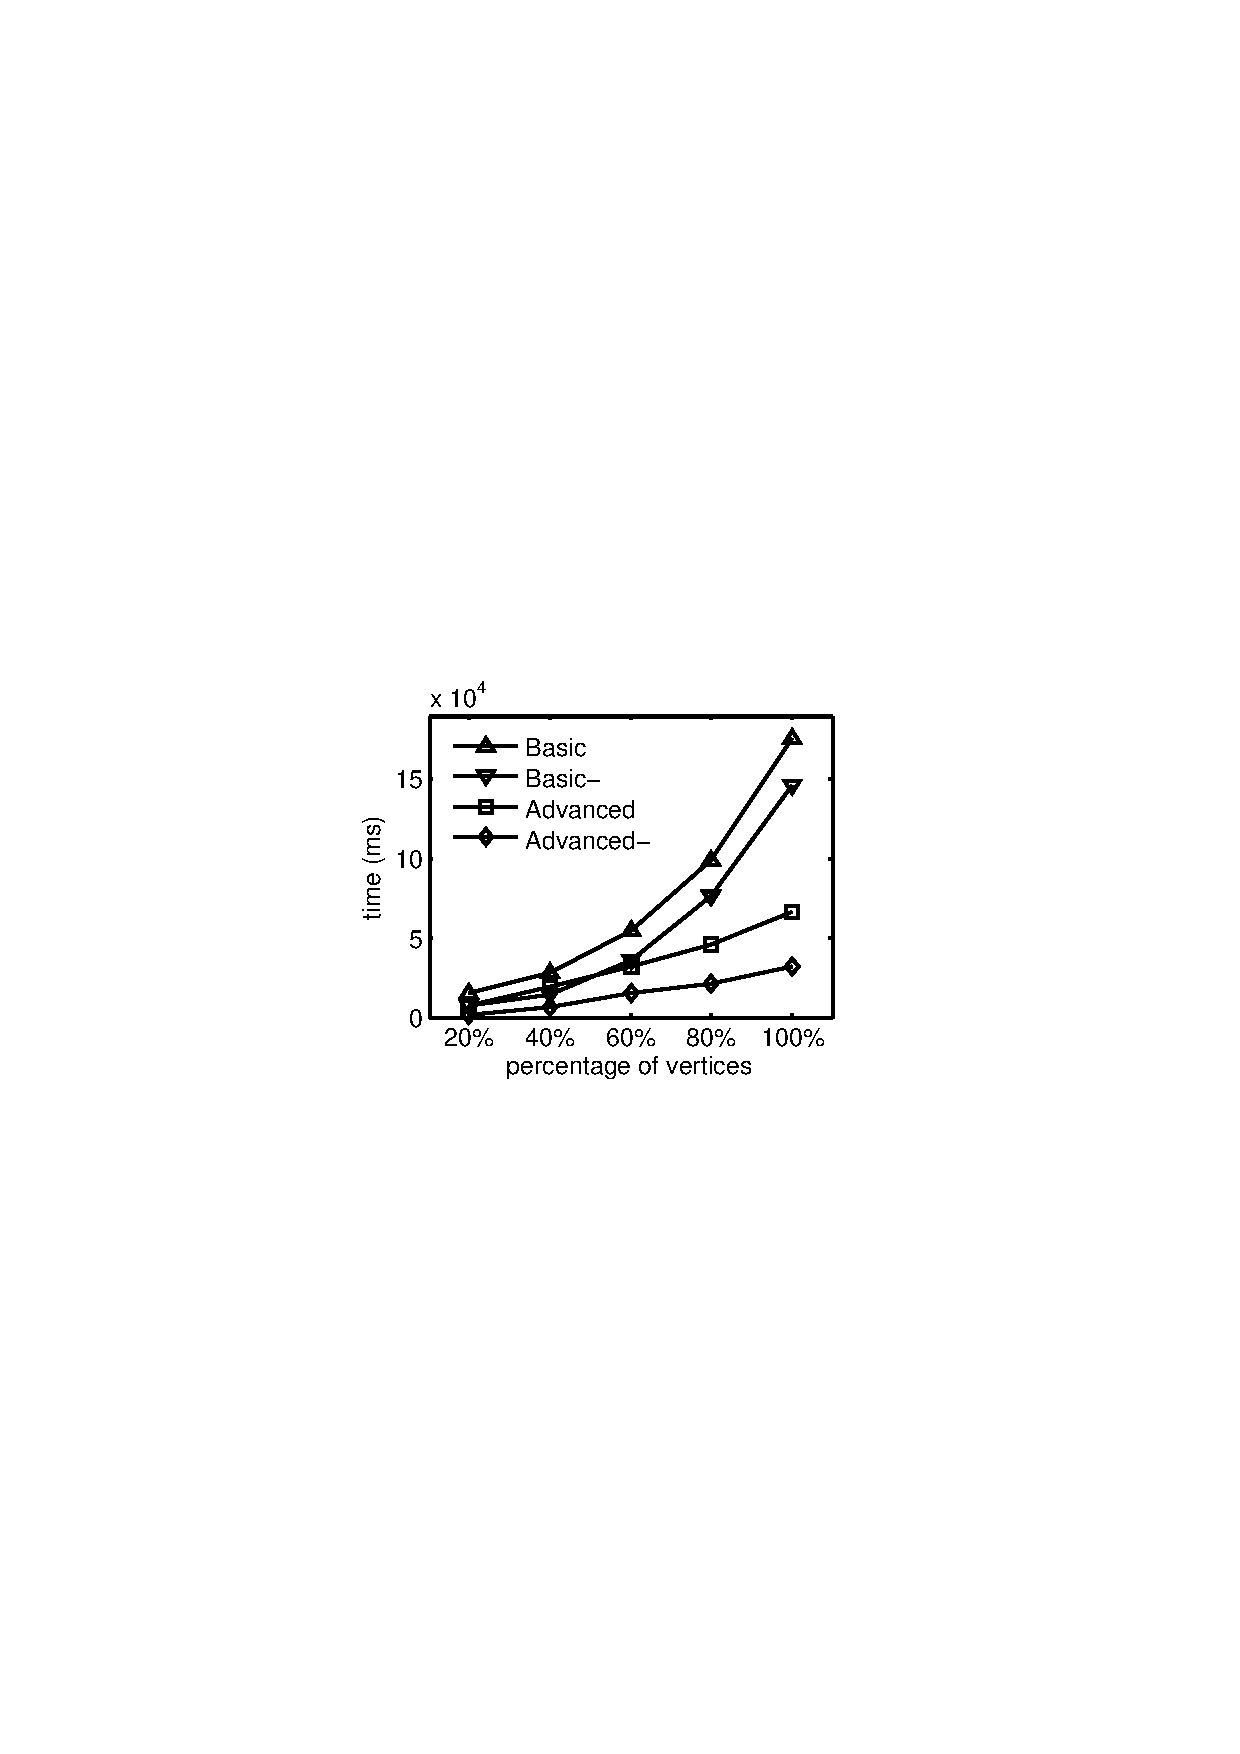
\includegraphics[width=3.725cm]{figures/dbpedia-index}
  \end{minipage}
  \\
  \small (a) Flickr (scalability)
  &
  \small (b) DBLP (scalability)
  &
  \small (c) Tencent (scalability)
  &
  \small (d) DBpedia (scalability)
\end{tabular}
\caption{Efficiency results of index construction.}
\label{fig:exp-index}
\end{figure*}



\begin{figure*}[htp]
\hspace*{-.4cm}
\centering
\begin{tabular}{c c c c}
  \begin{minipage}{3.76cm}
  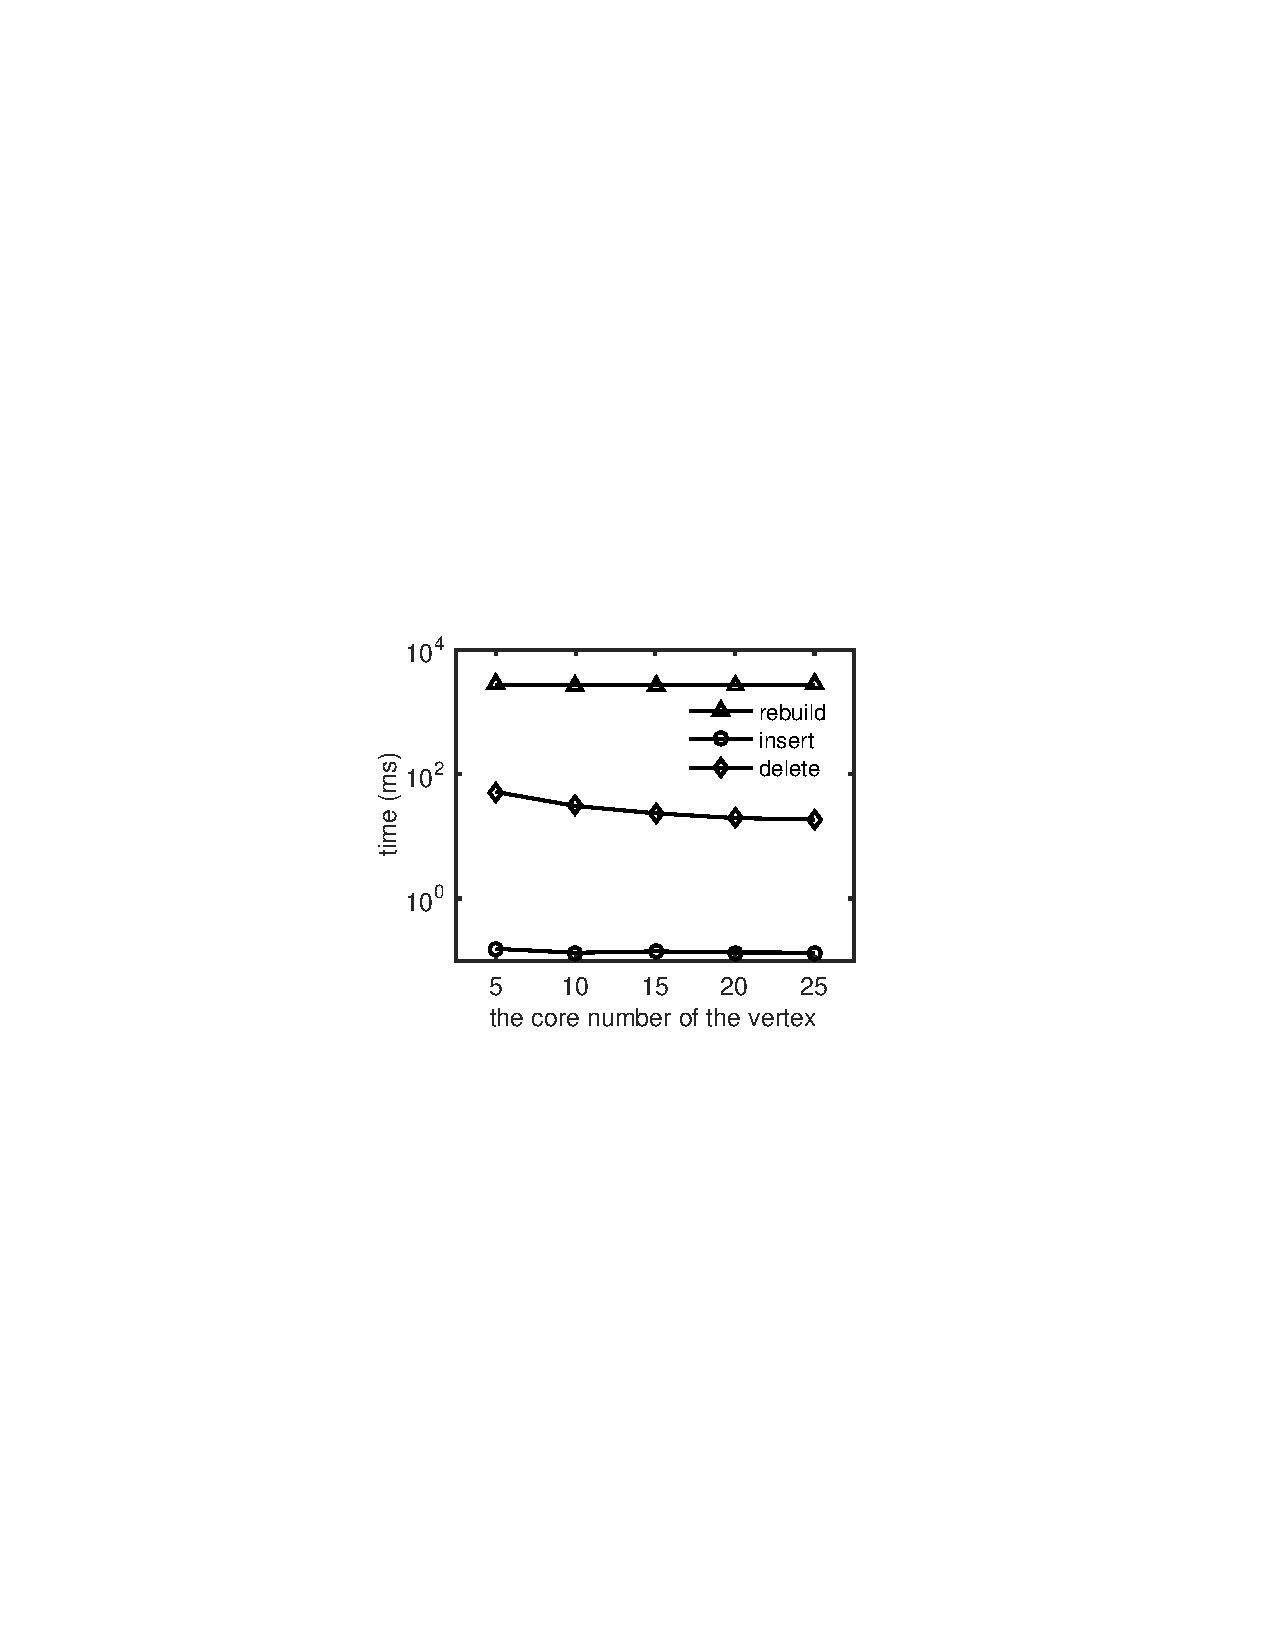
\includegraphics[width=3.725cm]{figures/flickrUpdate}
  \end{minipage}
  &
  \begin{minipage}{3.76cm}
  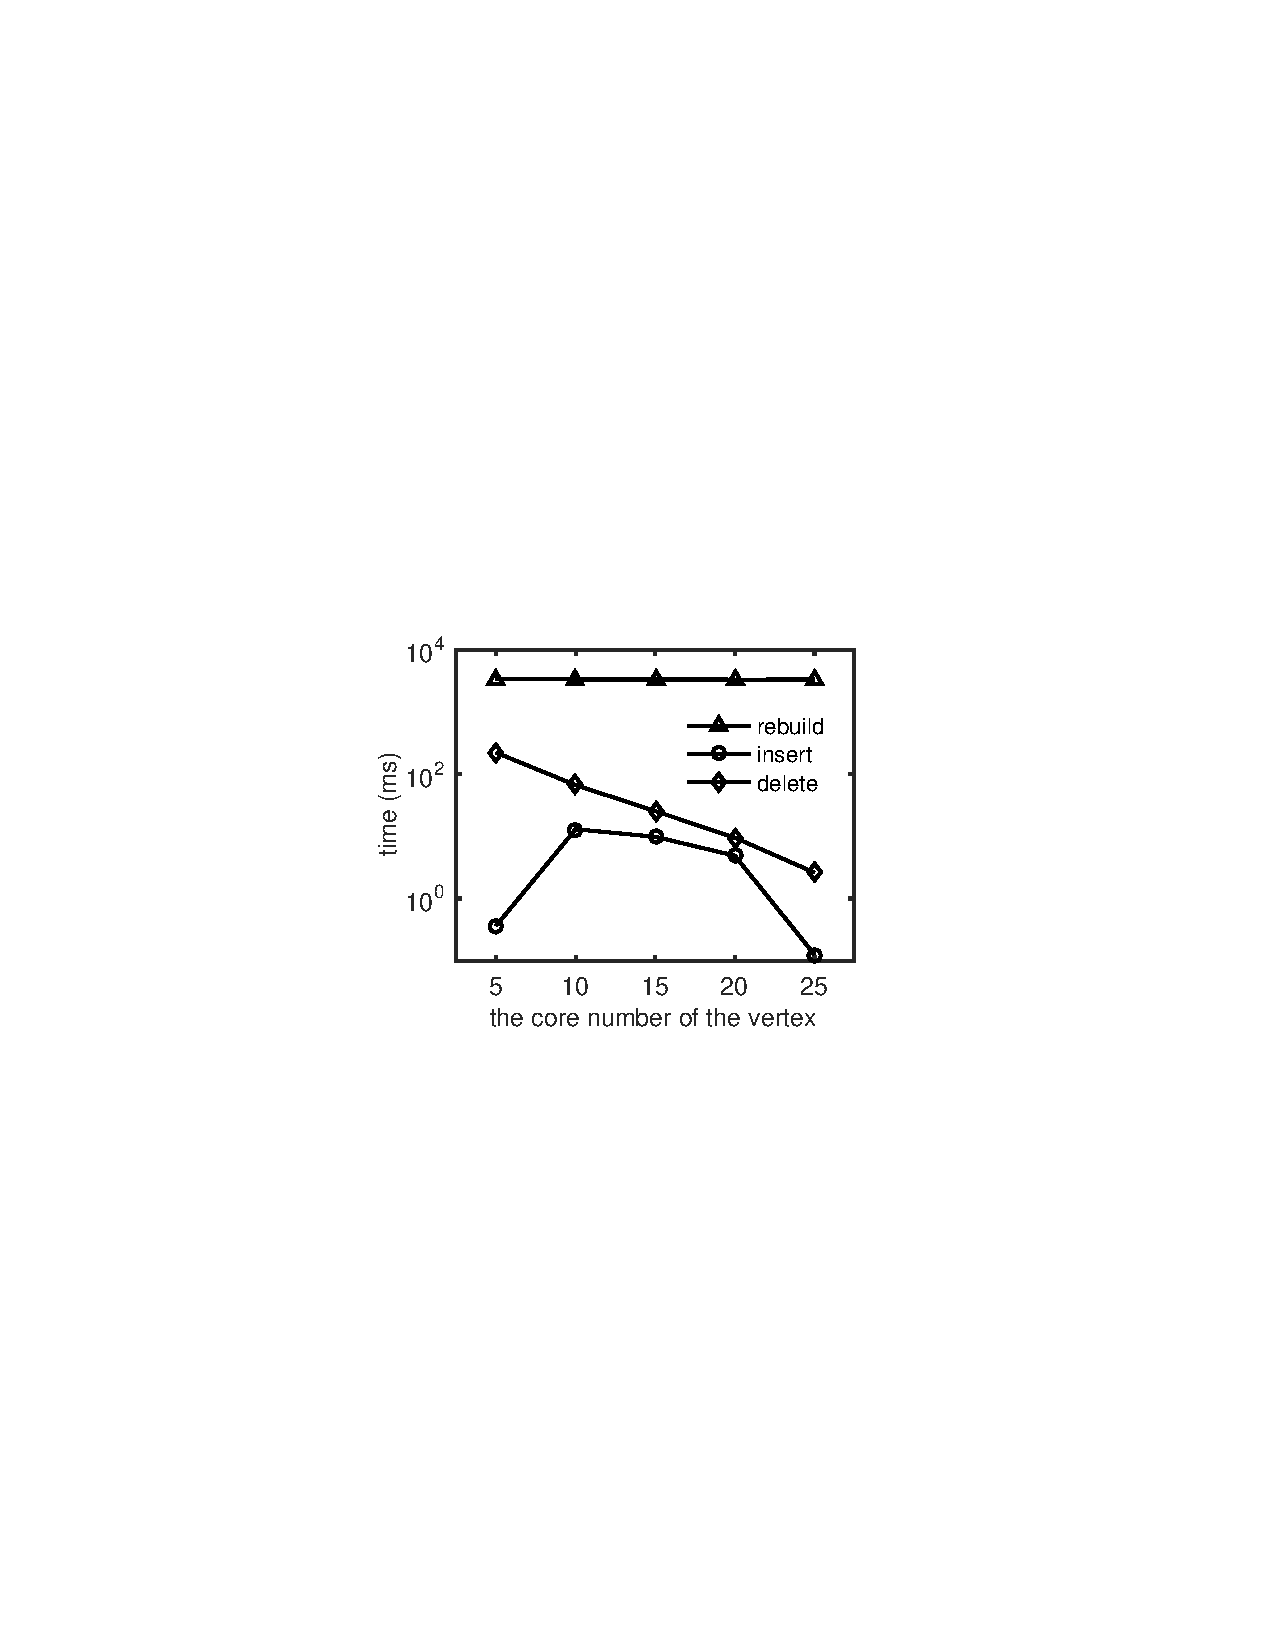
\includegraphics[width=3.725cm]{figures/dblpUpdate}
  \end{minipage}
  &
  \begin{minipage}{3.76cm}
  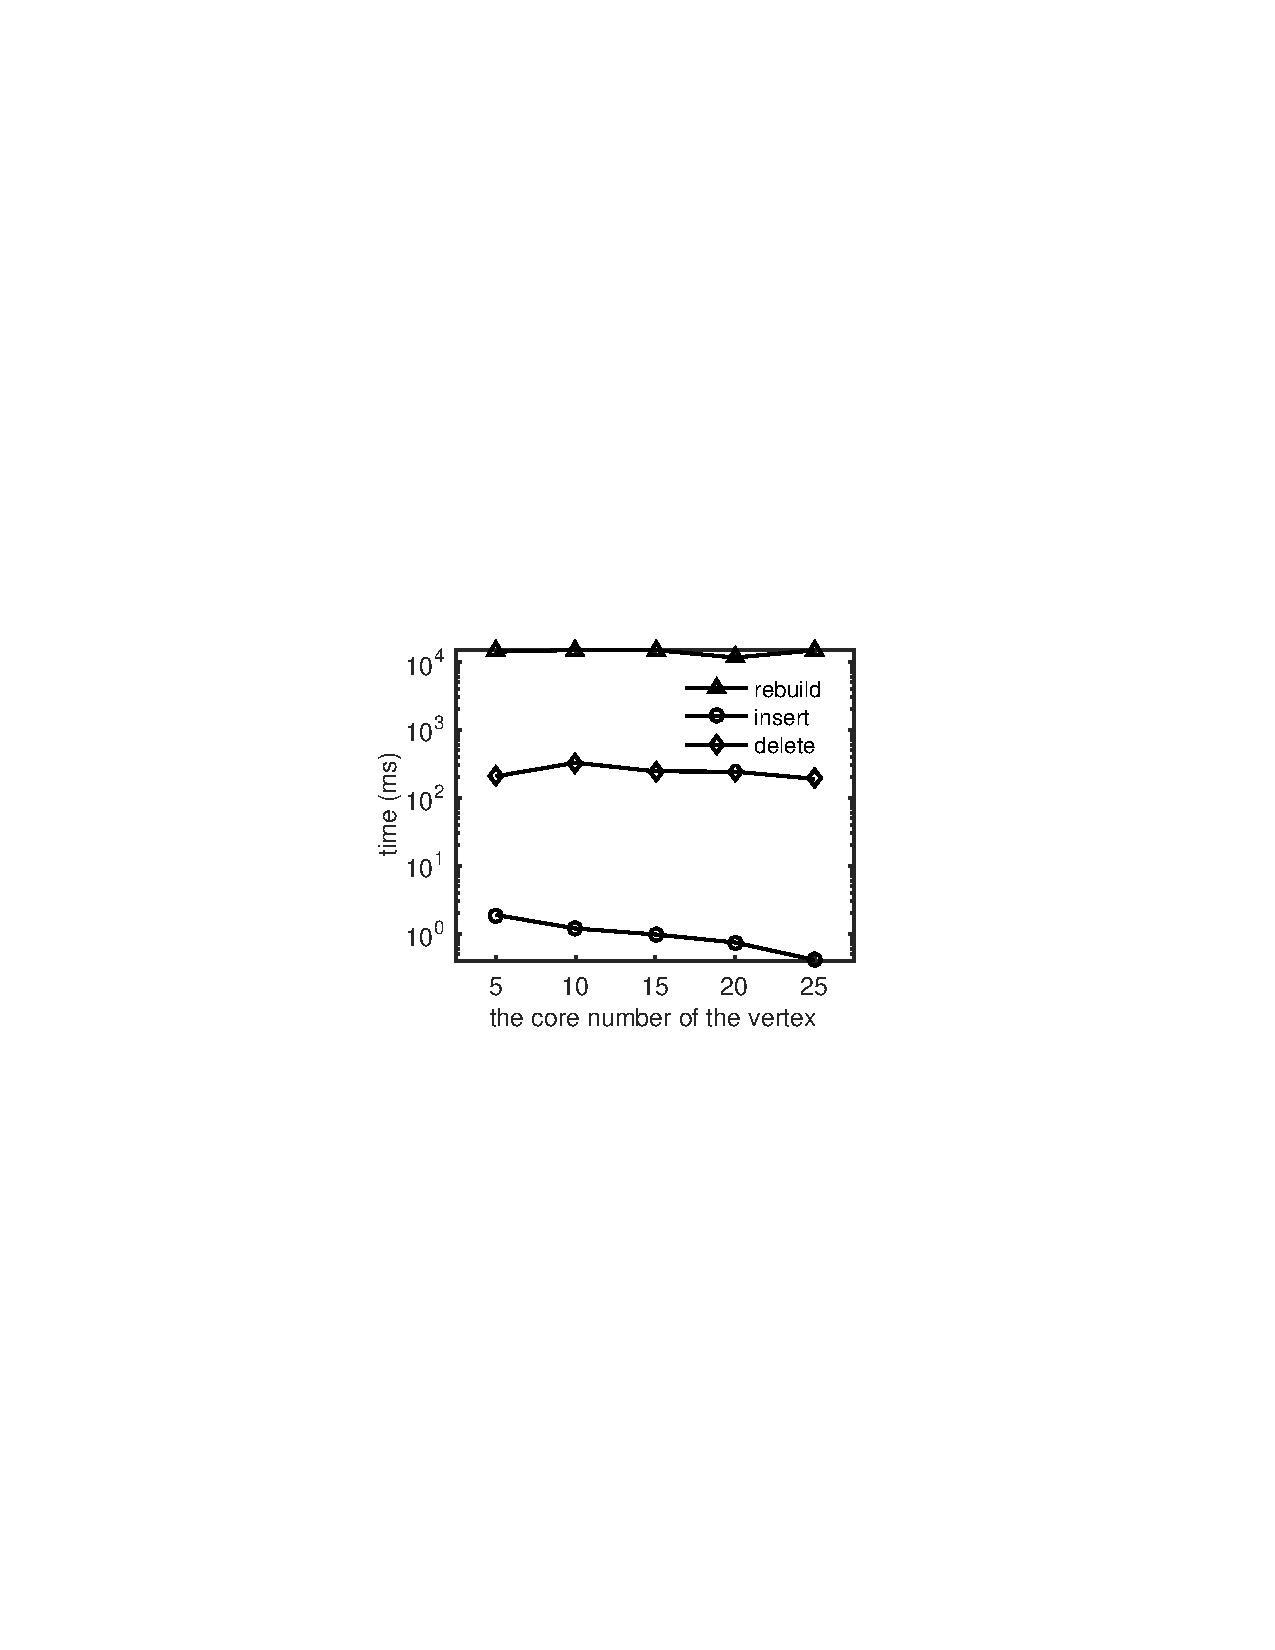
\includegraphics[width=3.725cm]{figures/tencentUpdate}
  \end{minipage}
  &
  \begin{minipage}{3.76cm}
  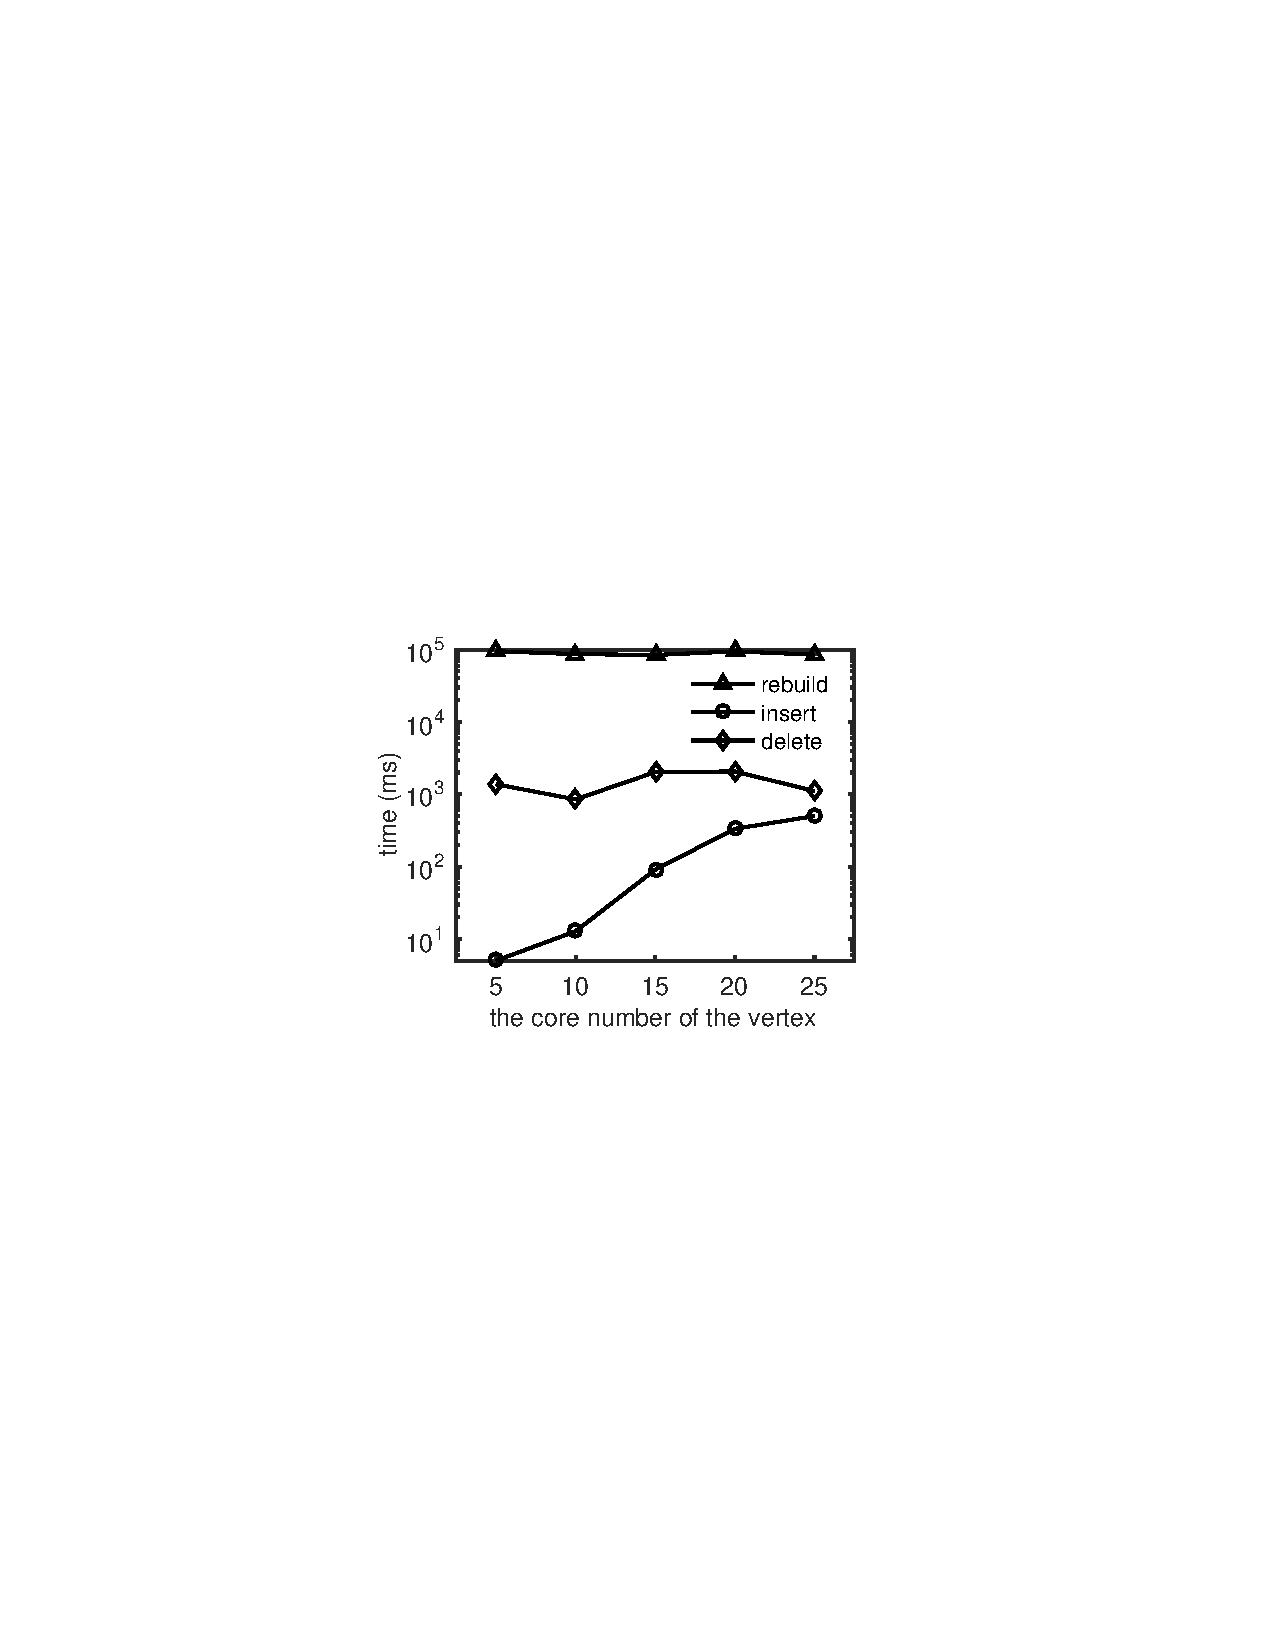
\includegraphics[width=3.725cm]{figures/dbpediaUpdate}
  \end{minipage}
  \\
  \small (a) Flickr (index maint.)
  &
  \small (b) DBLP (index maint.)
  &
  \small (c) Tencent (index maint.)
  &
  \small (d) DBpedia (index  maint.)
  \\
 \begin{minipage}{3.76cm}
  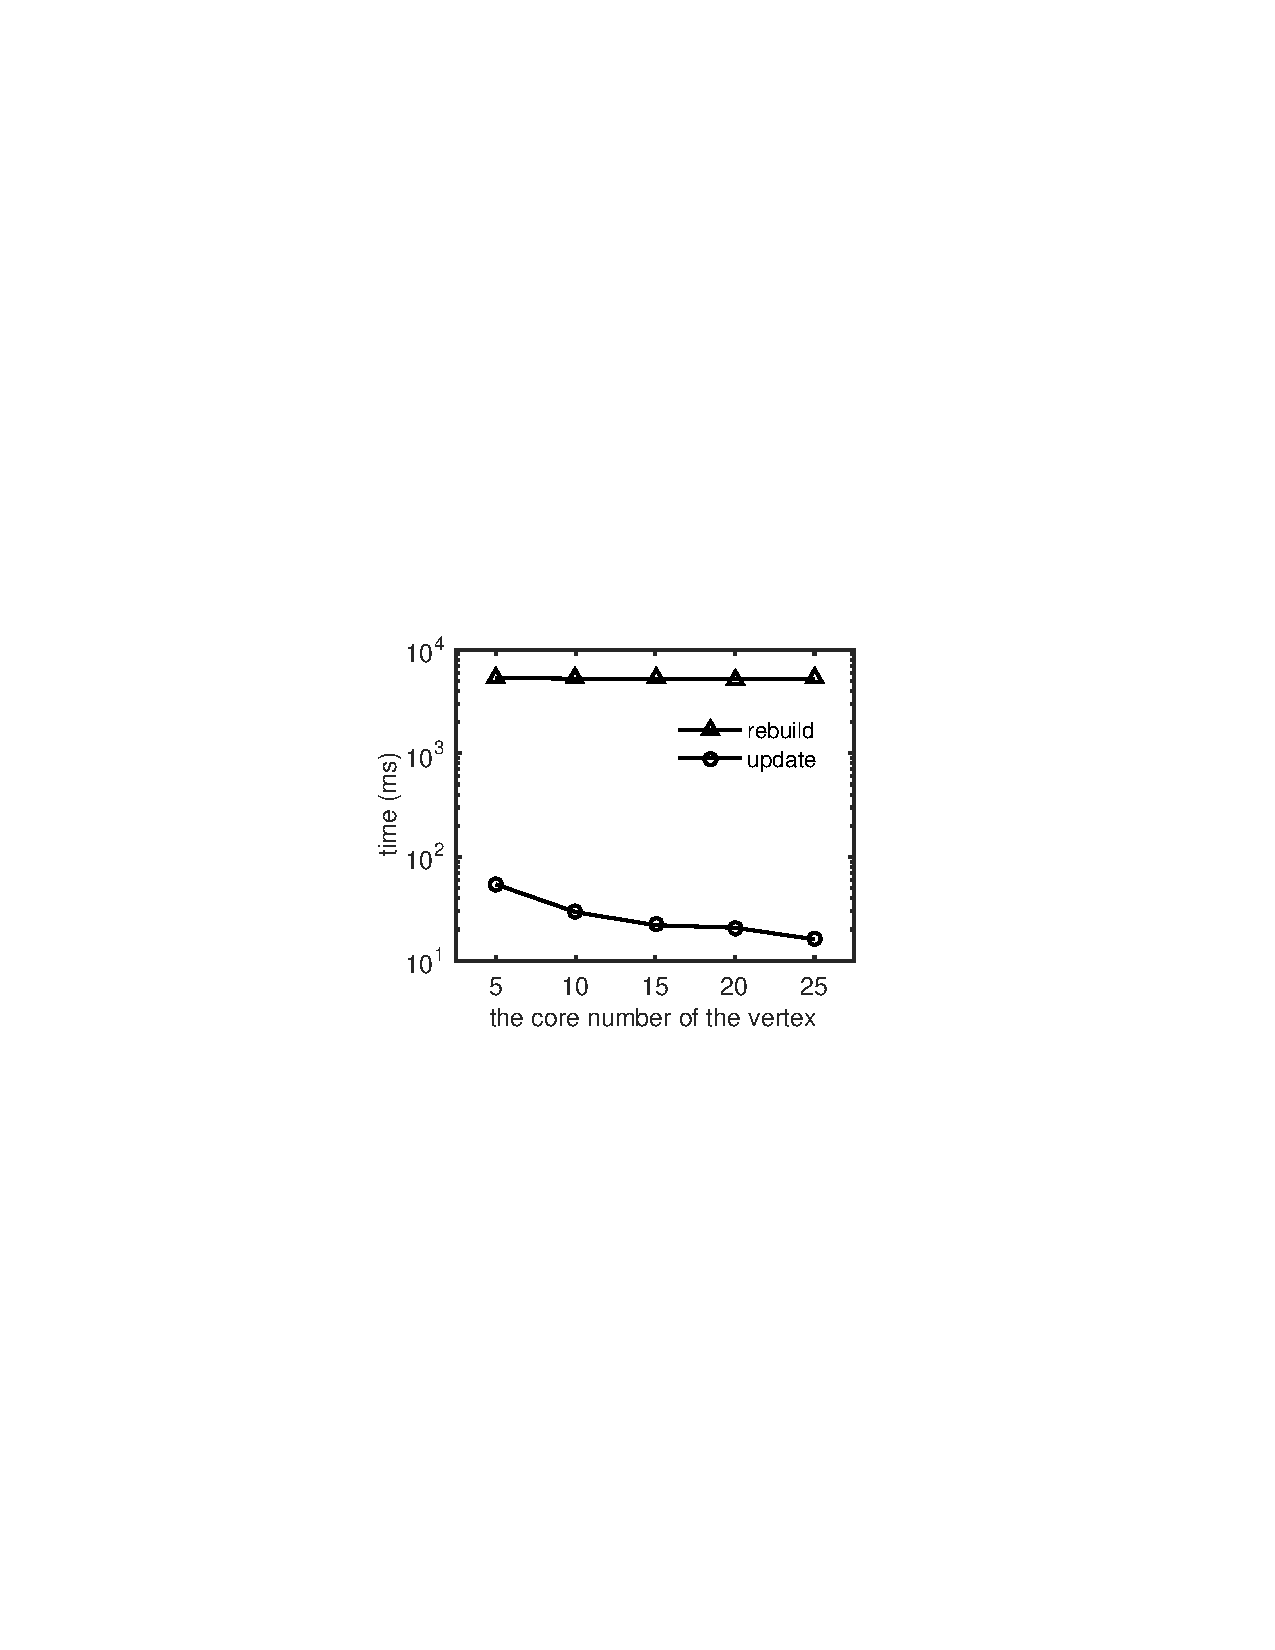
\includegraphics[width=3.725cm]{figures/flickrMix}
  \end{minipage}
  &
  \begin{minipage}{3.76cm}
  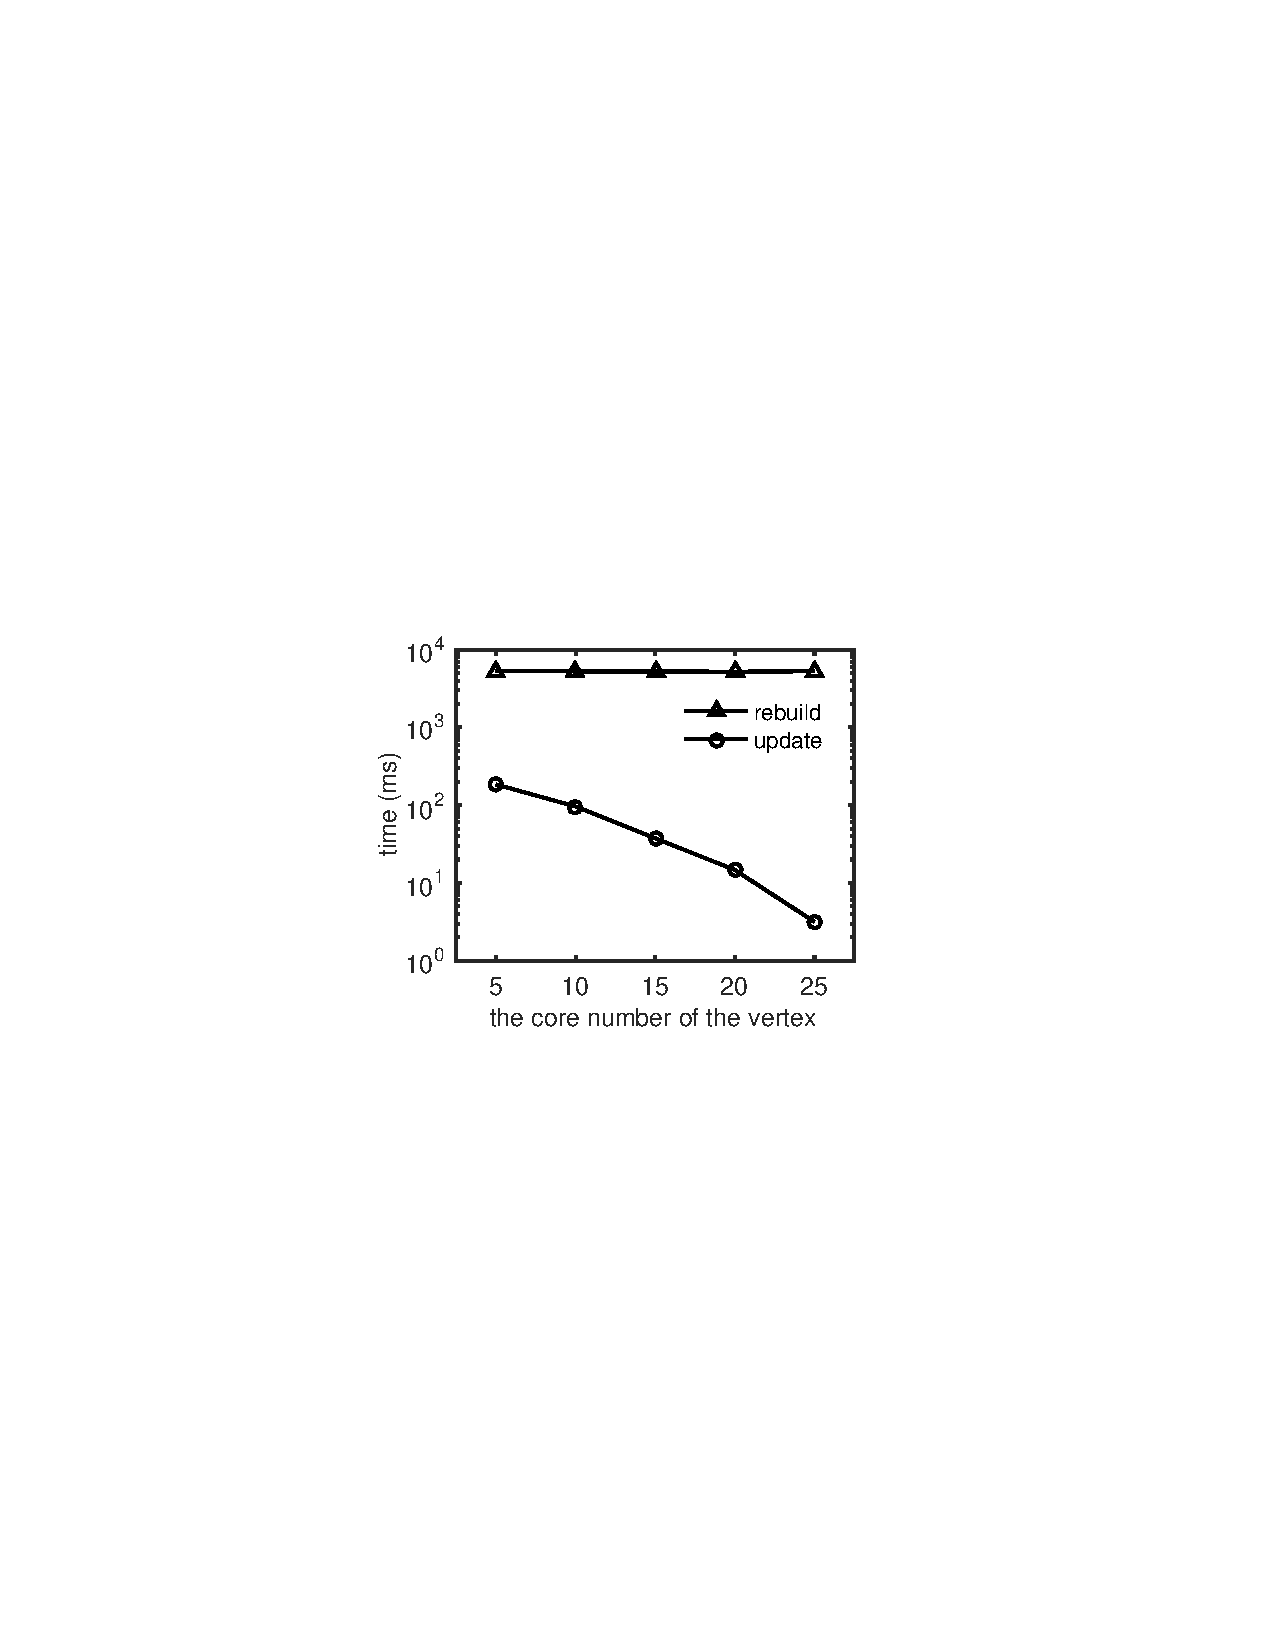
\includegraphics[width=3.725cm]{figures/dblpMix}
  \end{minipage}
  &
  \begin{minipage}{3.76cm}
  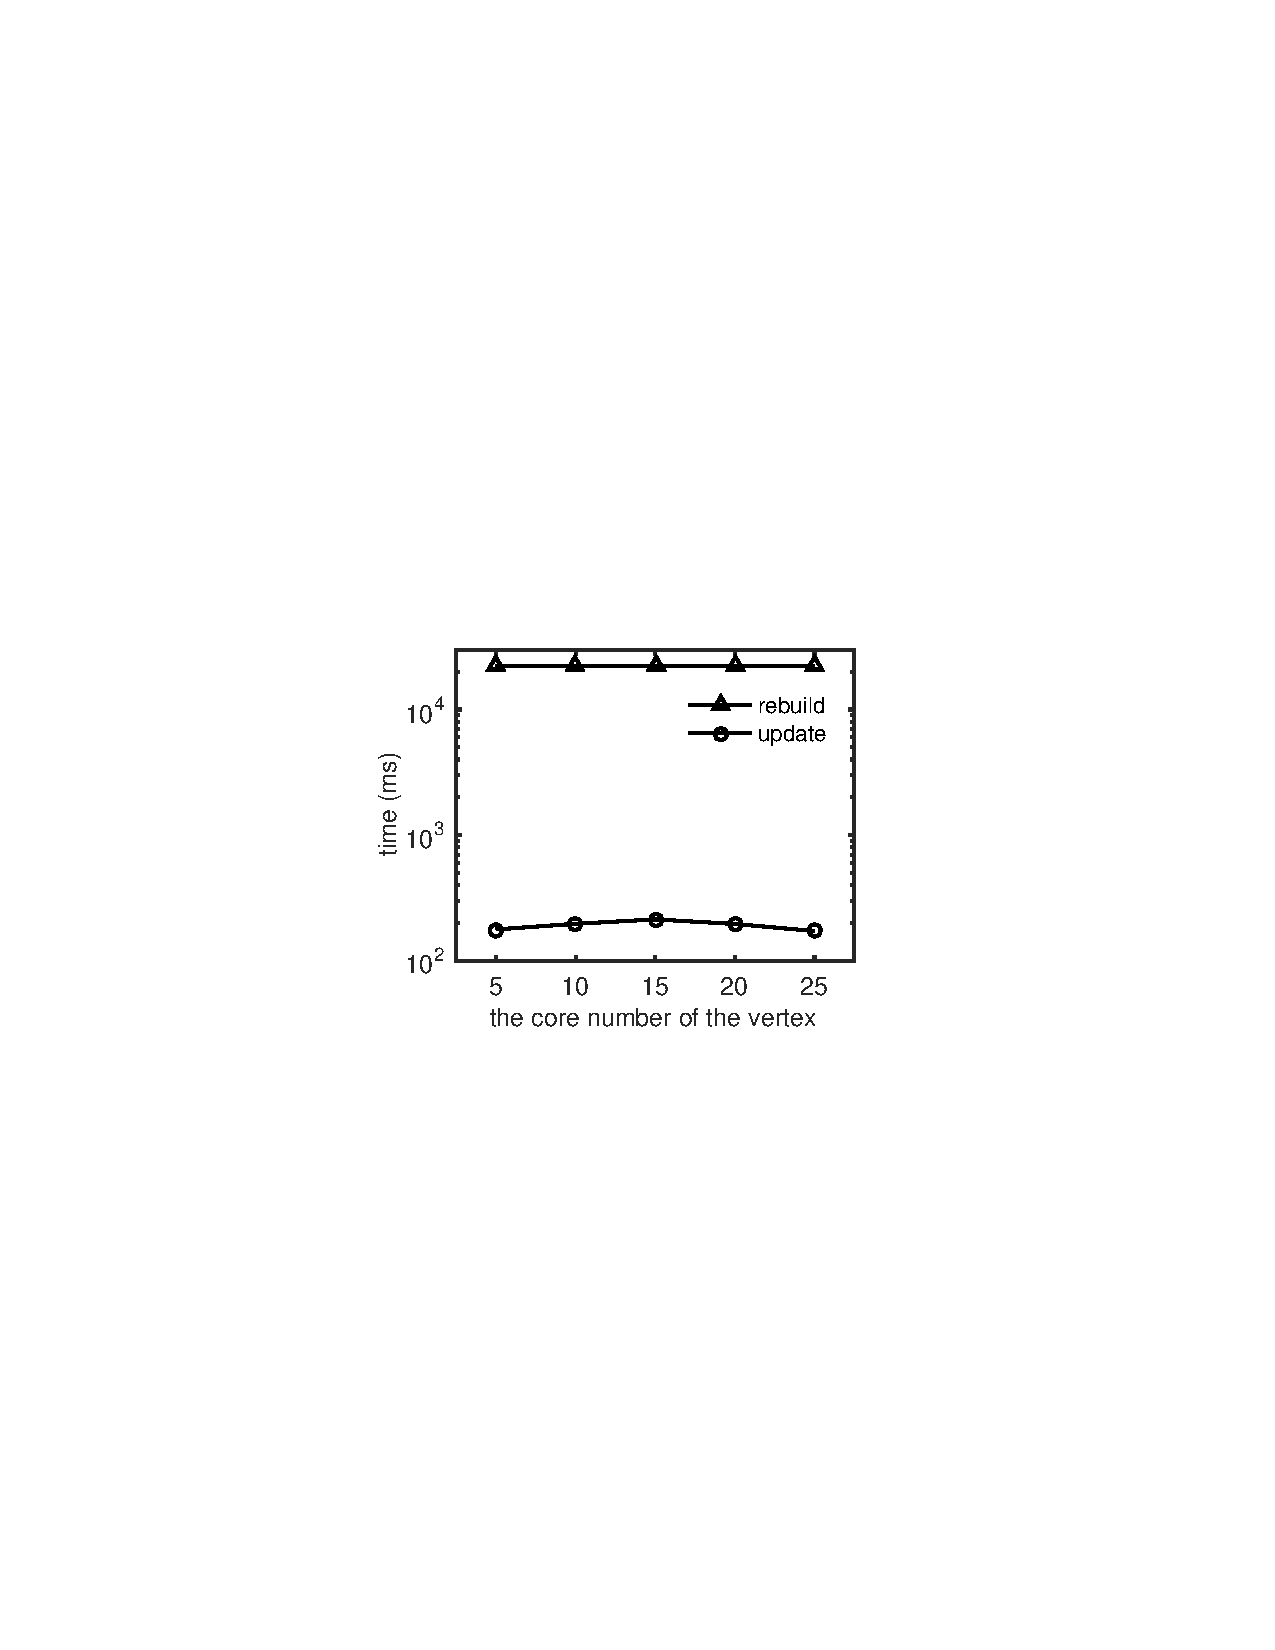
\includegraphics[width=3.725cm]{figures/tencentMix}
  \end{minipage}
  &
  \begin{minipage}{3.76cm}
  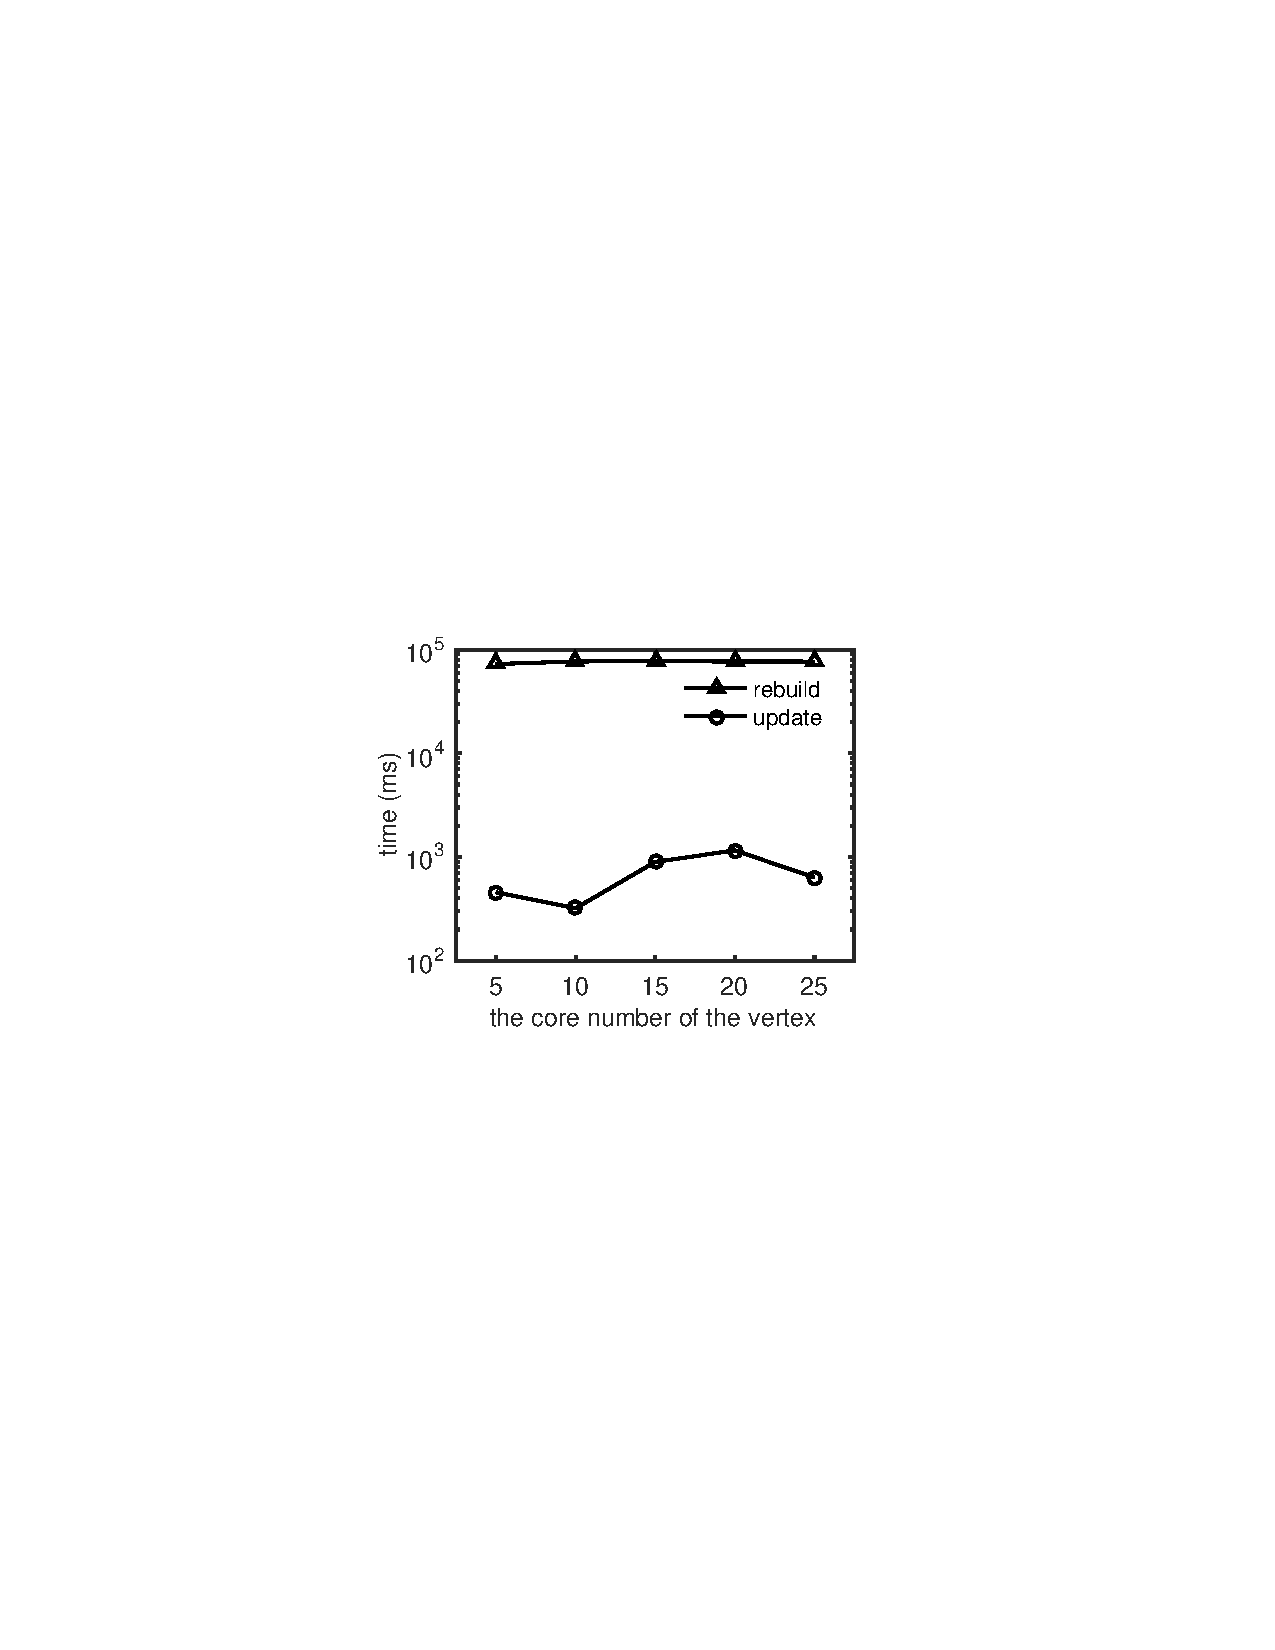
\includegraphics[width=3.725cm]{figures/dbpediaMix}
  \end{minipage}
  \\
  \small (e) Flickr (index maint.)
  &
  \small (f) DBLP (index maint.)
  &
  \small (g) Tencent (index maint.)
  &
  \small (h) DBpedia (index  maint.)
  \\
  &
 \begin{minipage}{3.325cm}
  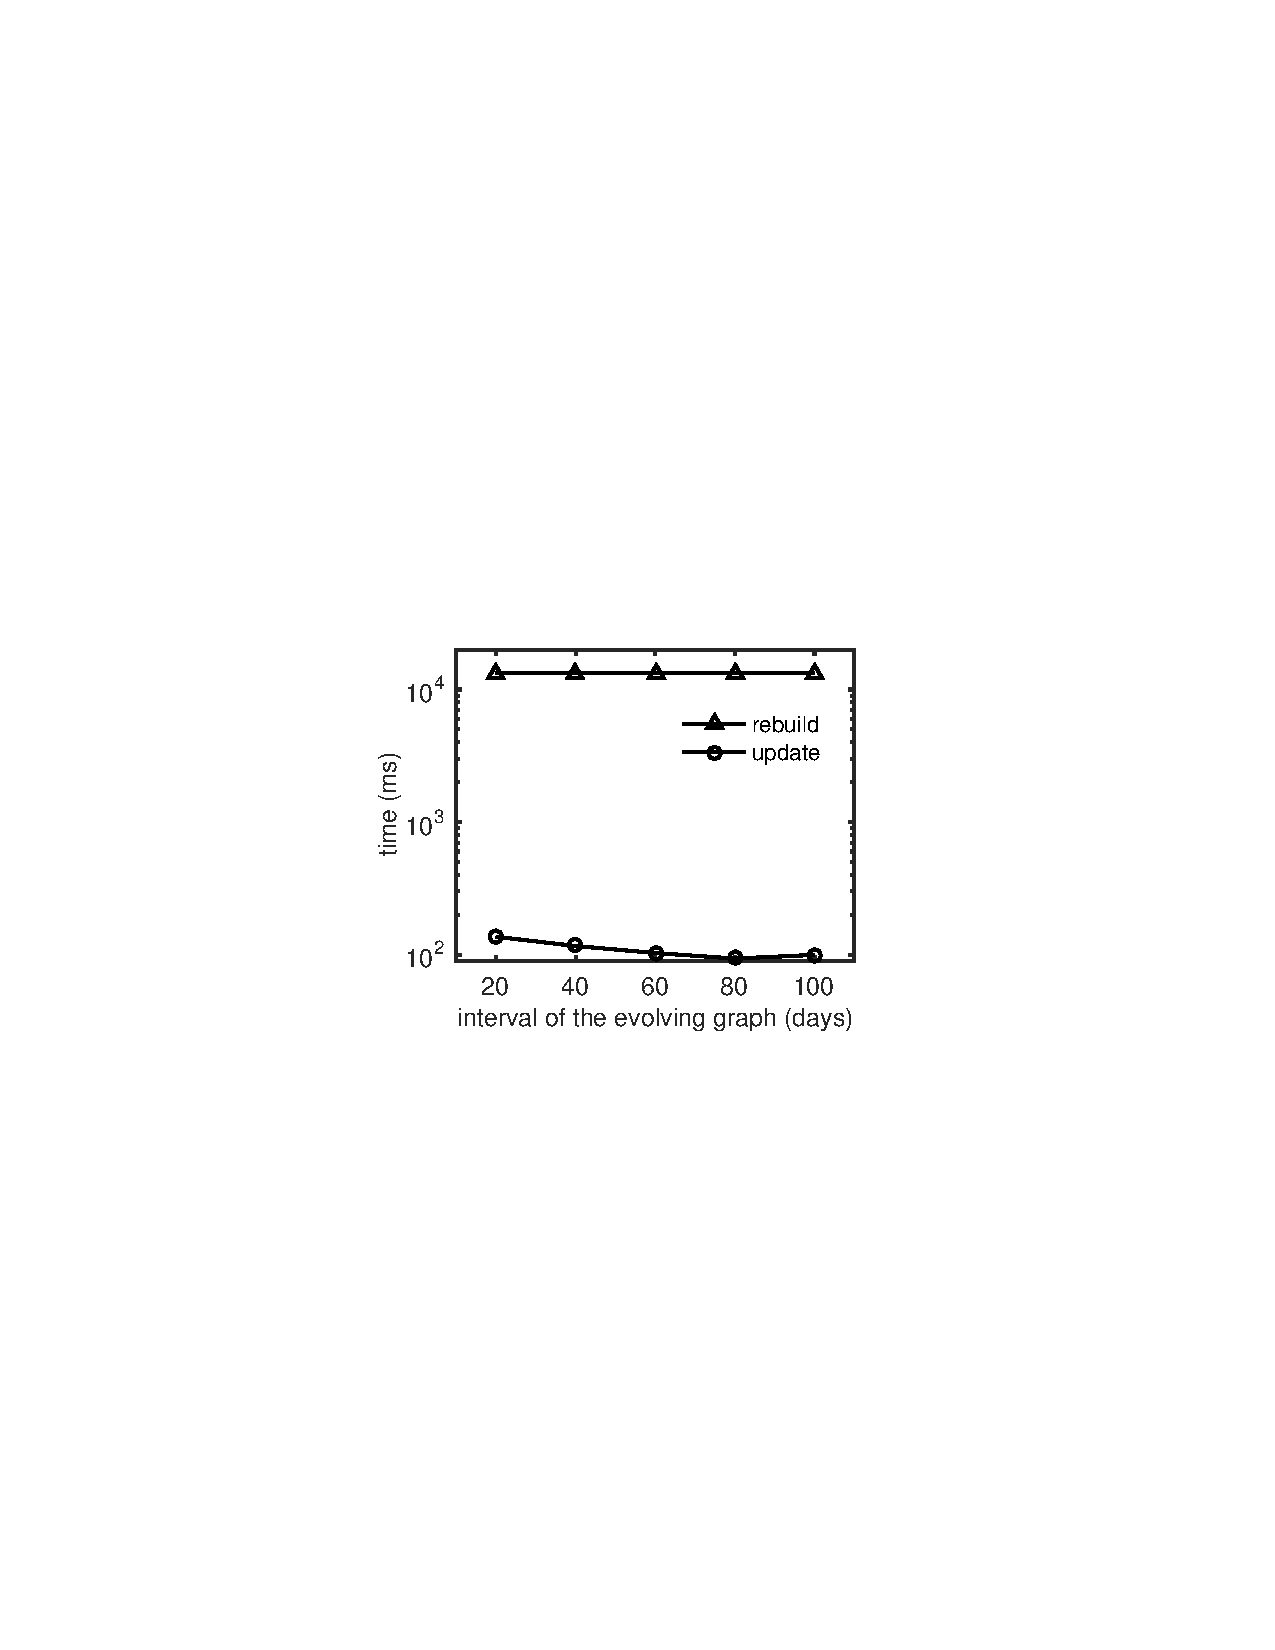
\includegraphics[width=3.725cm]{figures/DynamicFlickr}
  \end{minipage}
  &
  \begin{minipage}{3.325cm}
  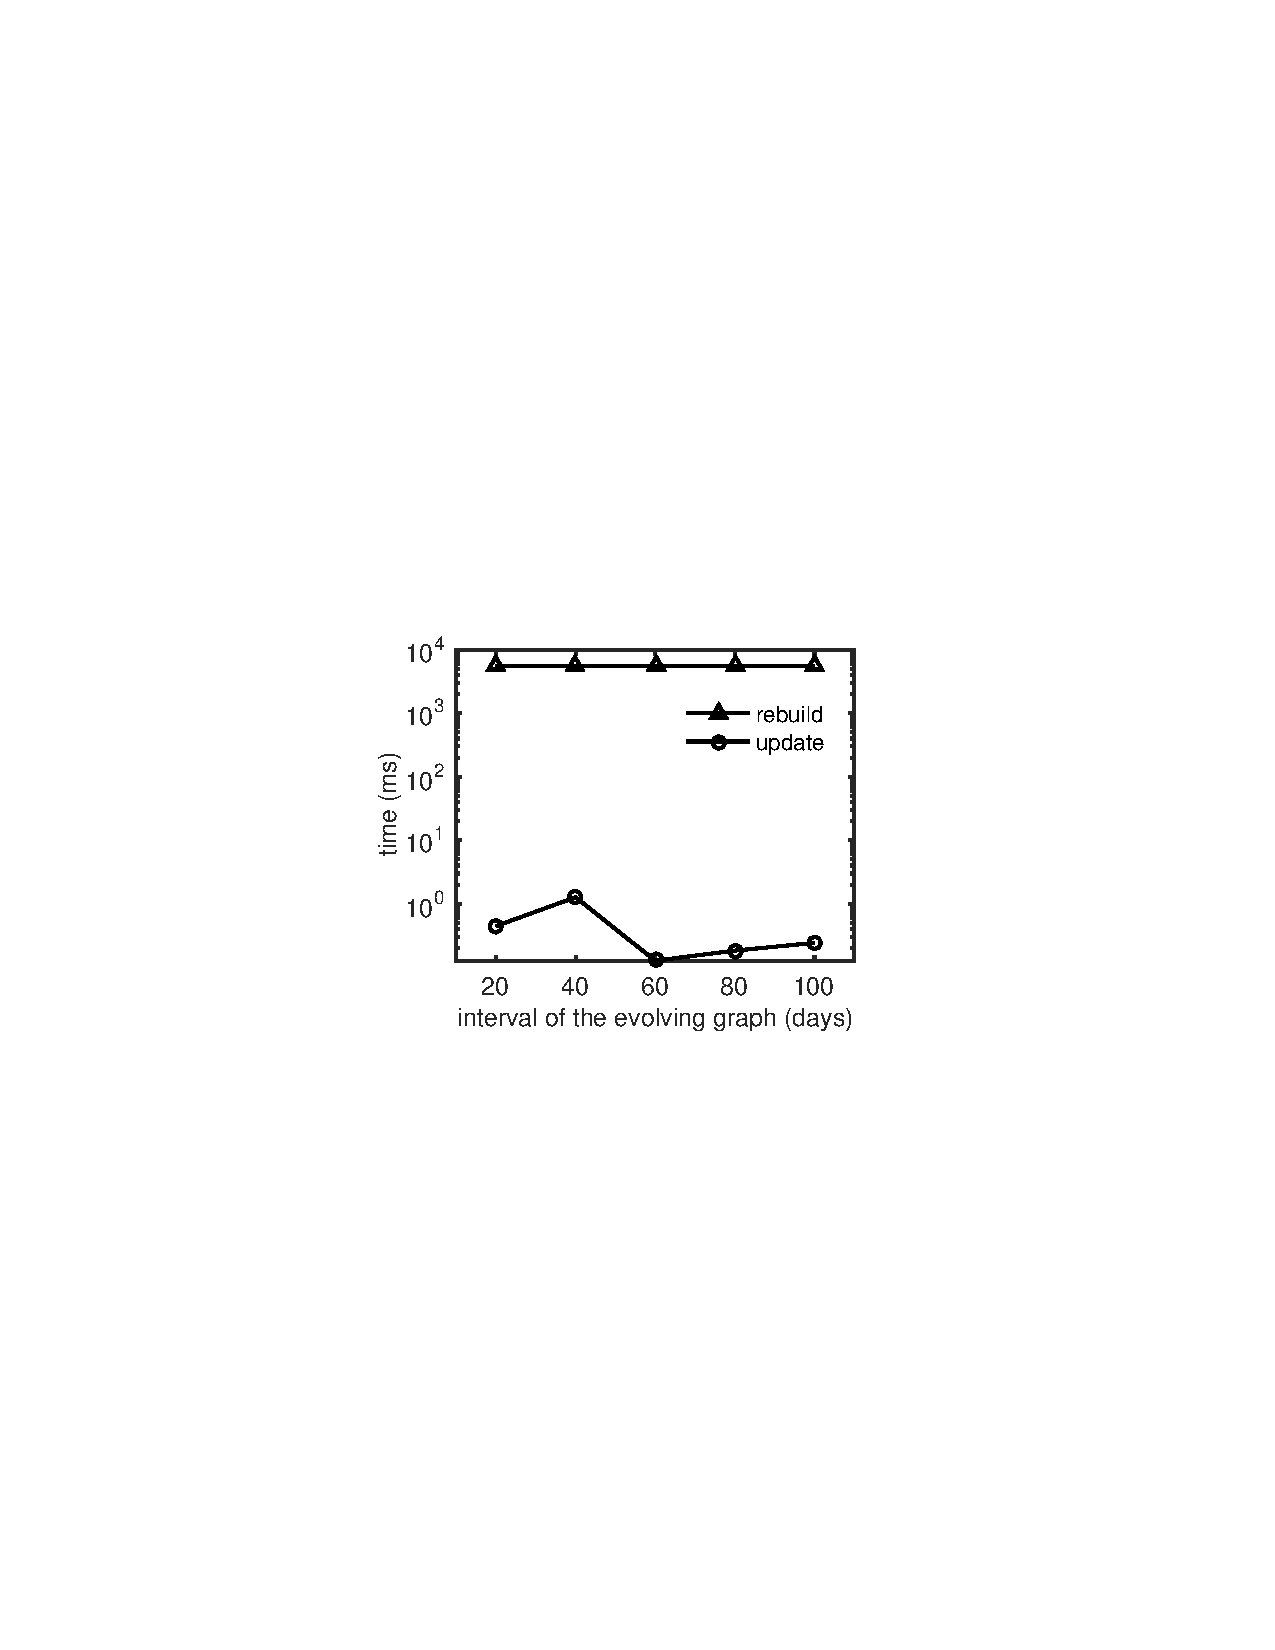
\includegraphics[width=3.725cm]{figures/DynamicYoutube}
  \end{minipage}
  \\
  &
  \small (i) DFlickr
  &
  \small (j) Youtube
  &
\\
\end{tabular}
\caption{Efficiency results of index maintenance.}
\label{fig:exp-indexMaintenance}
\end{figure*}


\begin{figure*}[htp]
\hspace*{-.4cm}
\centering
\begin{tabular}{c c c c}
      \begin{minipage}{3.725cm}
	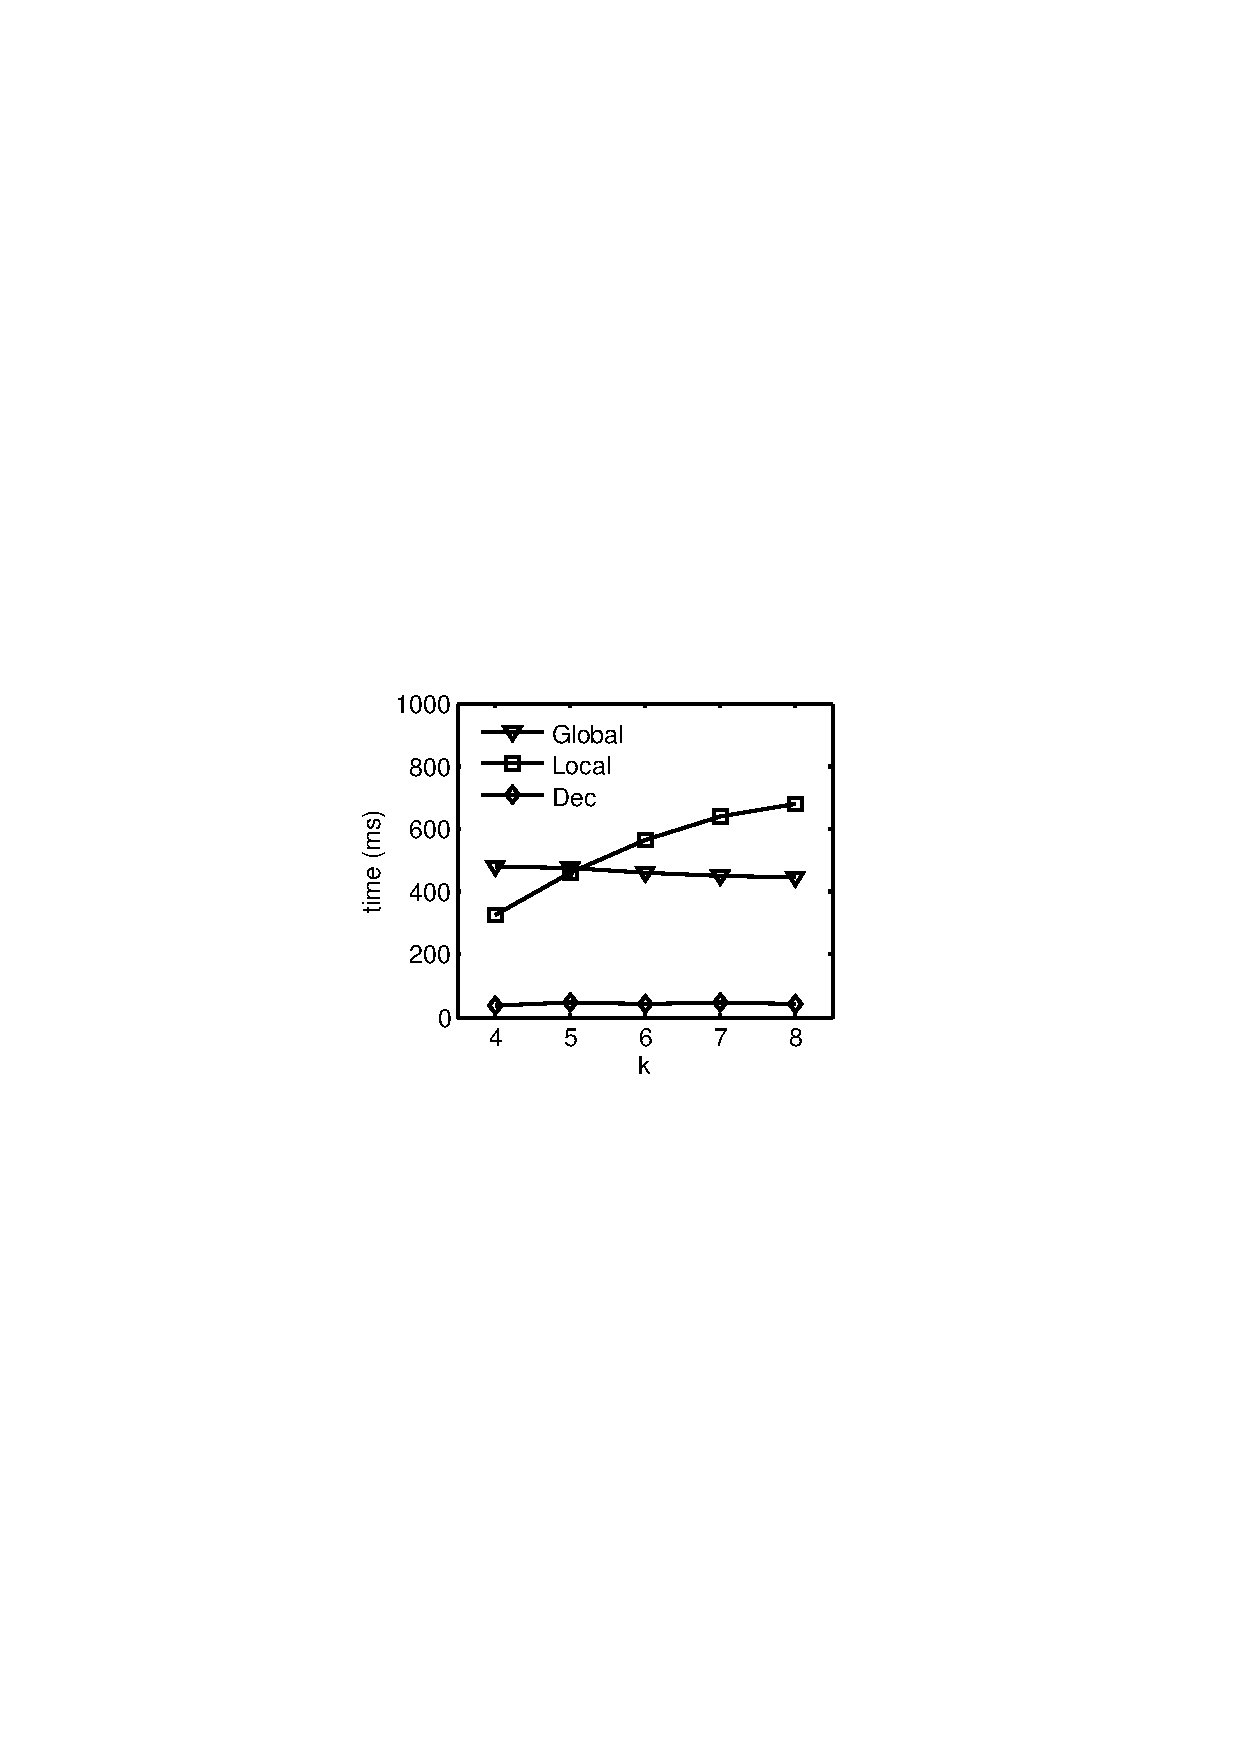
\includegraphics[width=3.725cm]{figures/flickr-comp}
  \end{minipage}
  &
  \begin{minipage}{3.725cm}
	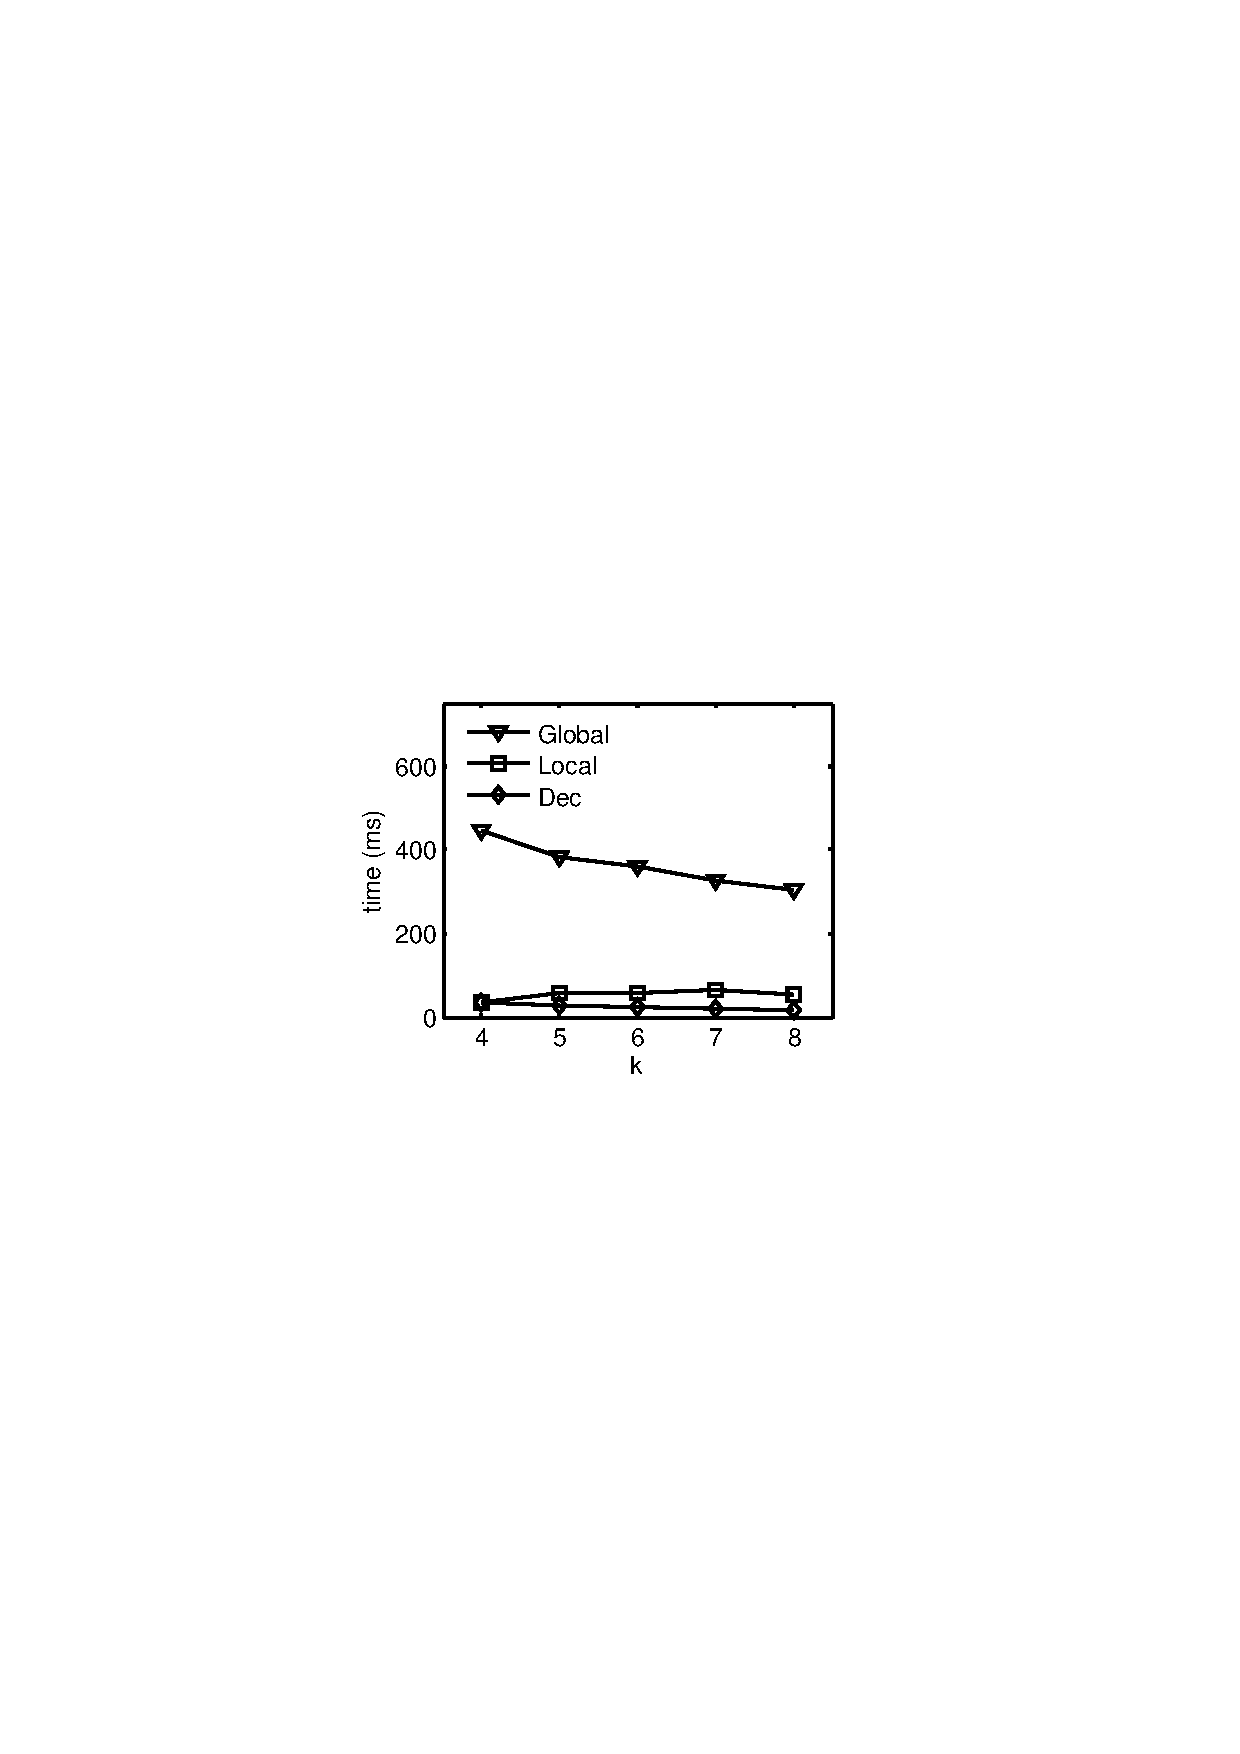
\includegraphics[width=3.725cm]{figures/dblp-comp}
  \end{minipage}
  &
  \begin{minipage}{3.725cm}
	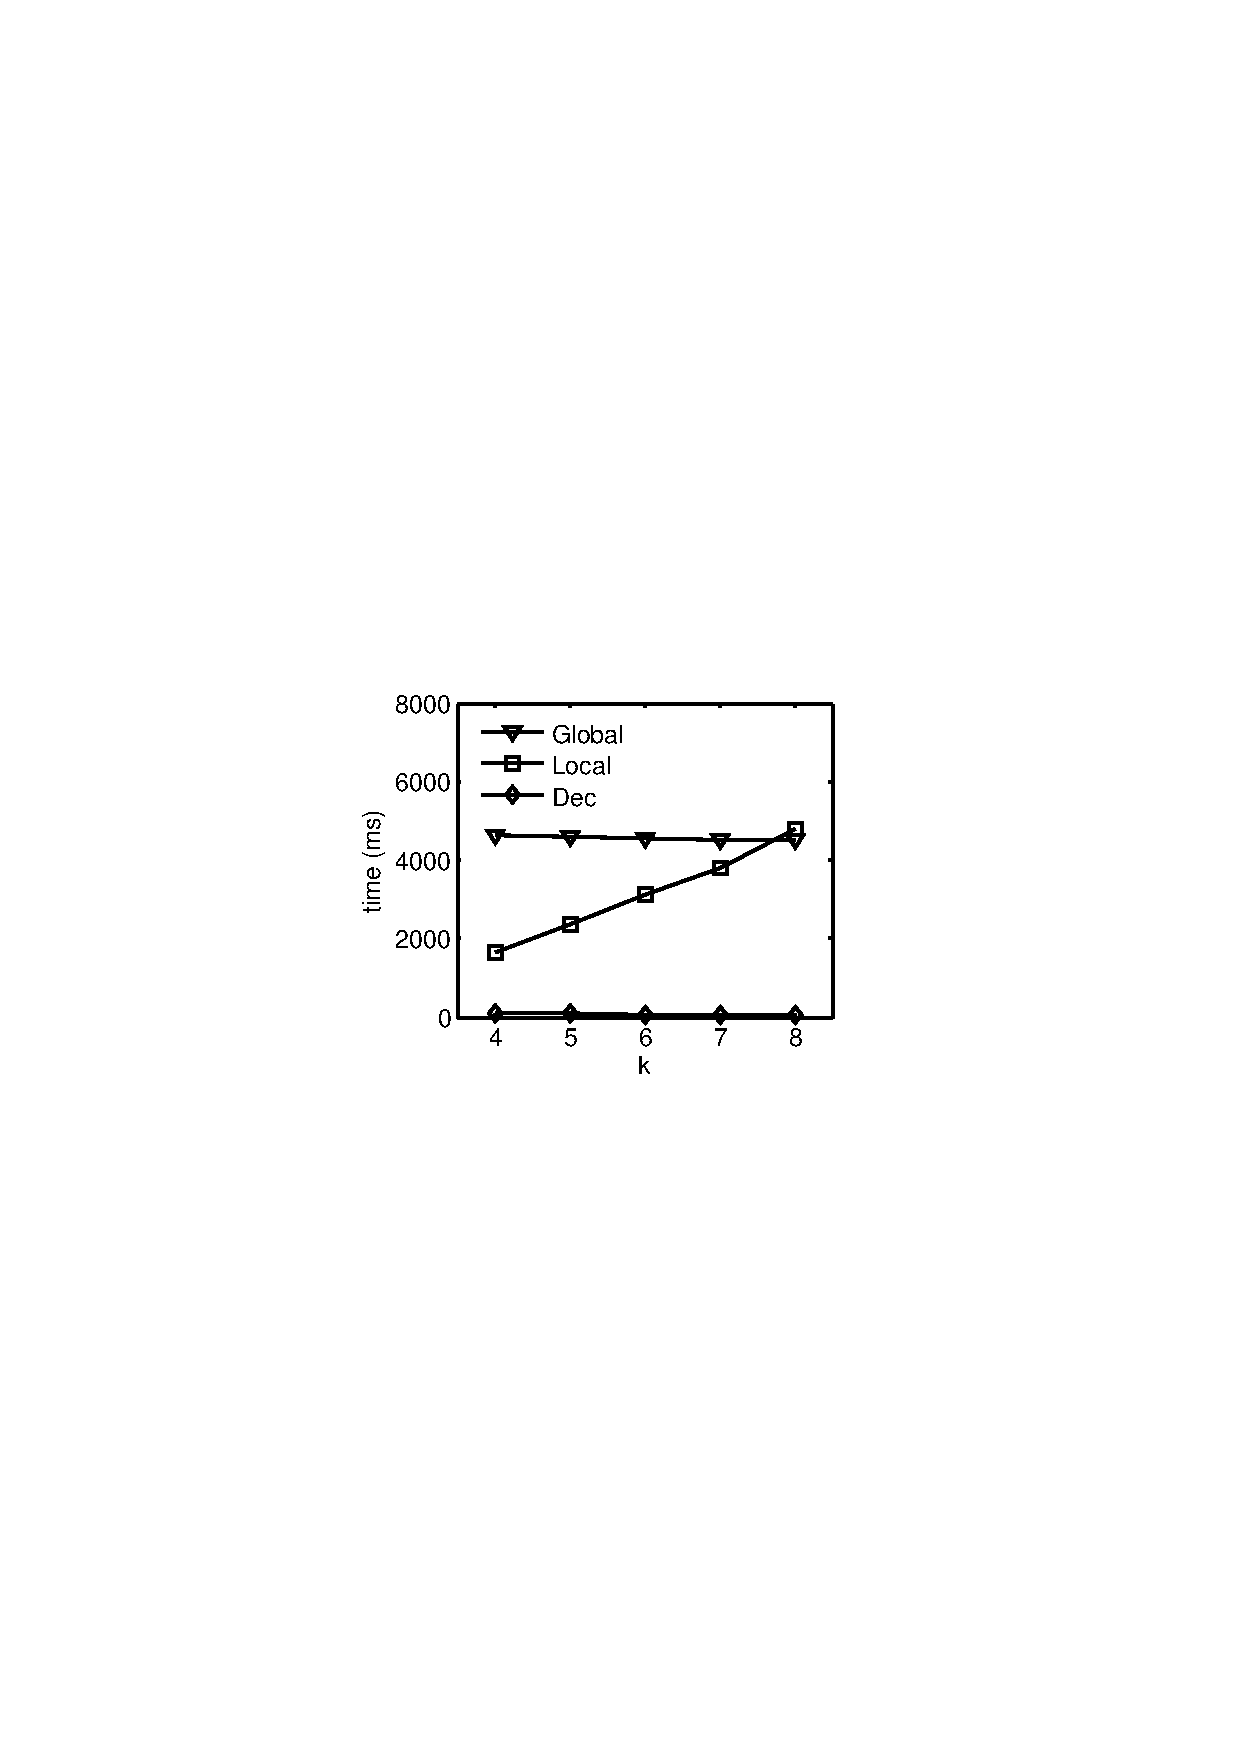
\includegraphics[width=3.725cm]{figures/tencent-comp}
  \end{minipage}
  &
  \begin{minipage}{3.725cm}
	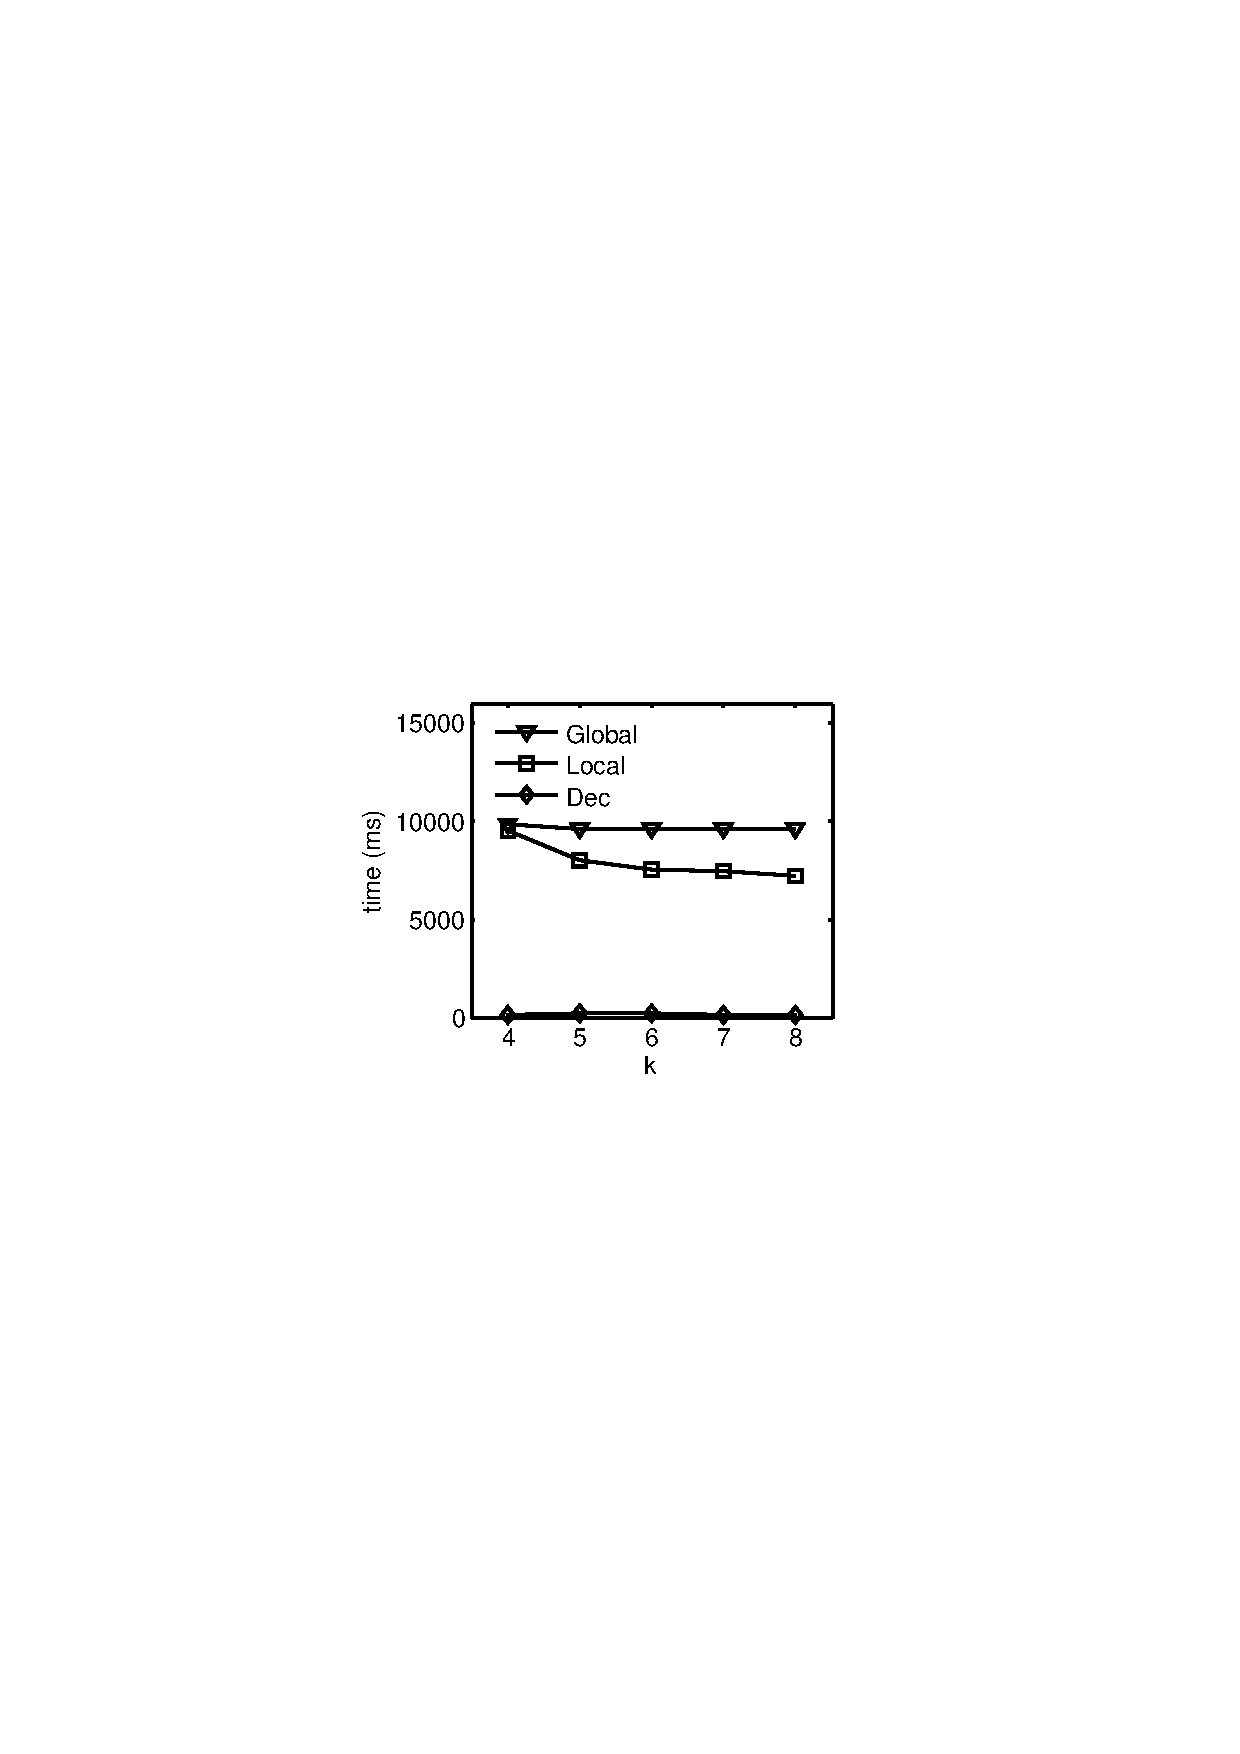
\includegraphics[width=3.725cm]{figures/dbpedia-comp}
  \end{minipage}
  \\
  \small (a) Flickr (efficiency)
  &
  \small (b) DBLP (efficiency)
  &
  \small (c) Tencent (efficiency)
  &
  \small (d) DBpedia (efficiency)
  \\

  \begin{minipage}{3.725cm}
	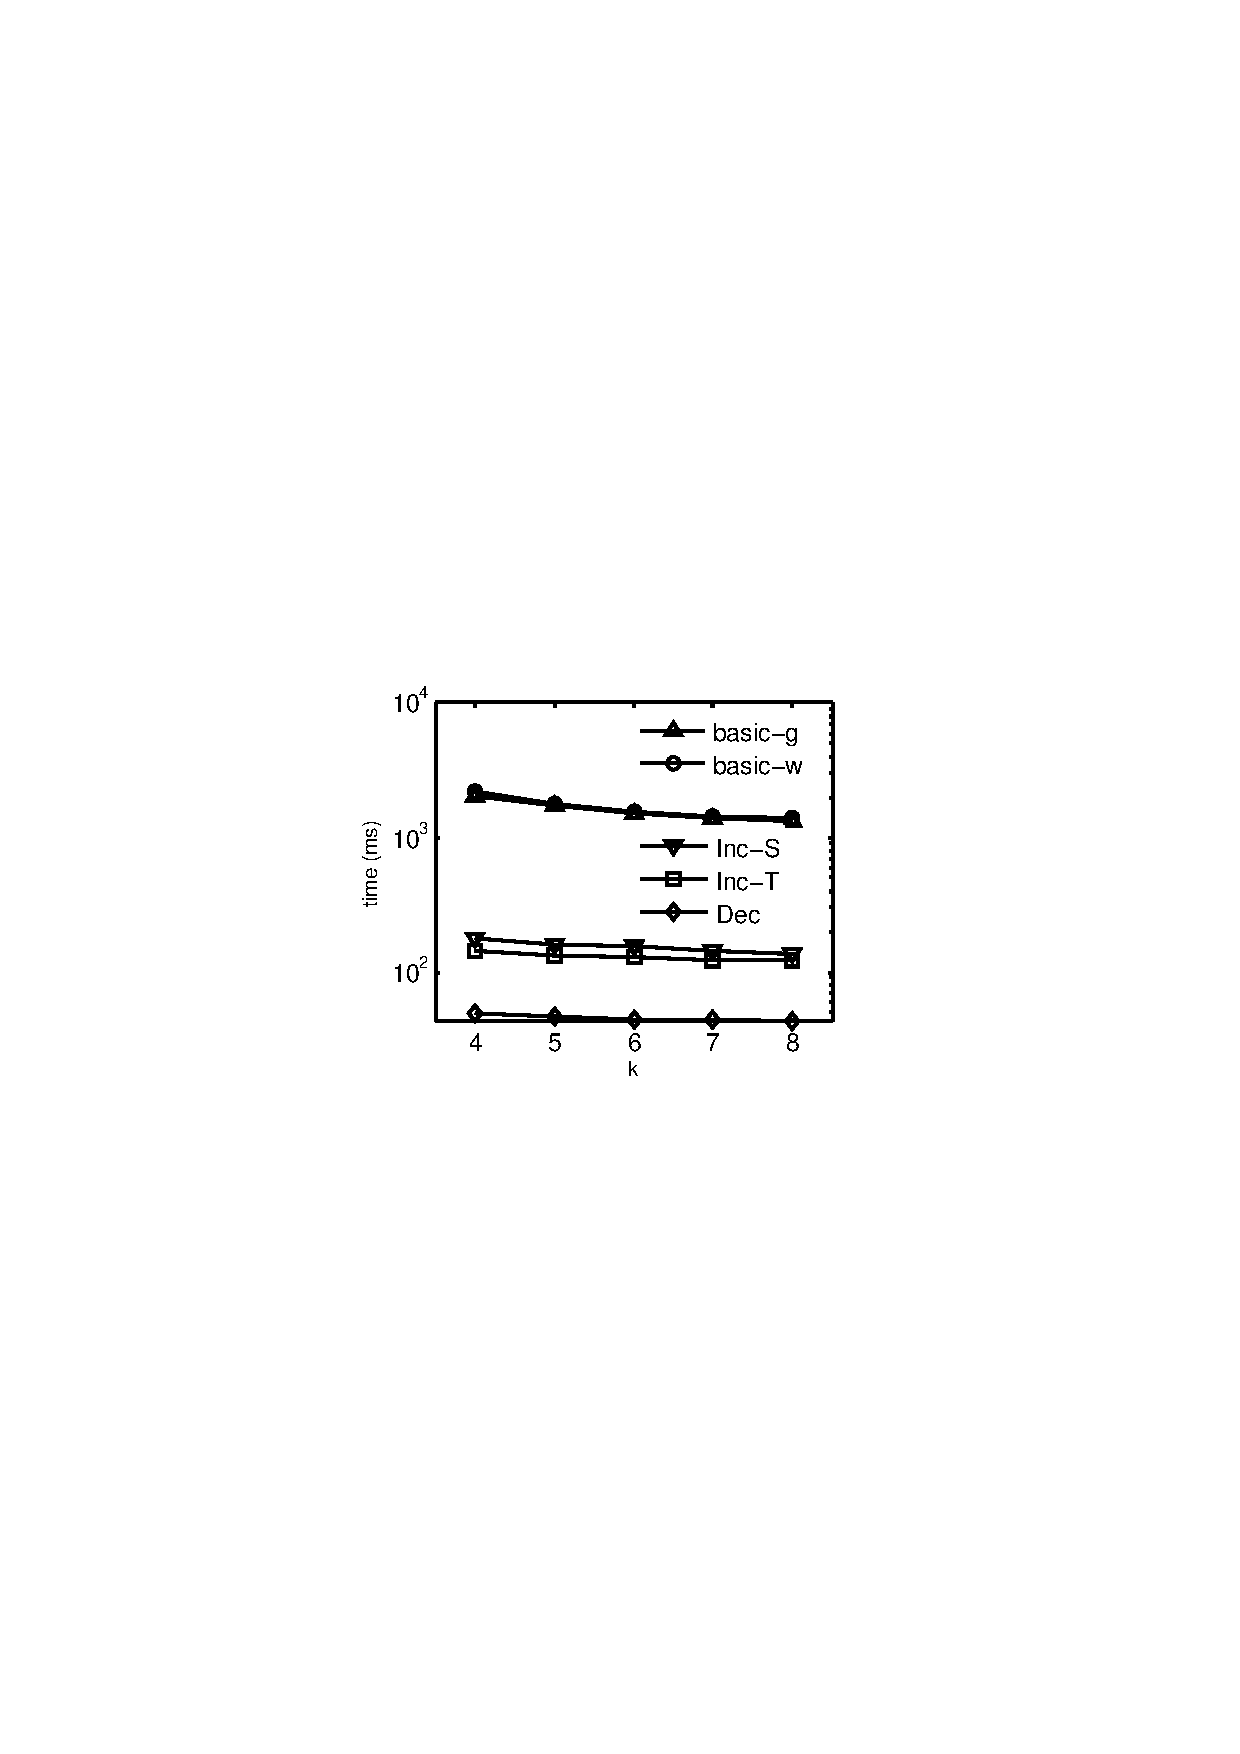
\includegraphics[width=3.725cm]{figures/flickr-k}
  \end{minipage}
  &
  \begin{minipage}{3.725cm}
	\includegraphics[width=3.725cm]{figures/dblp-k}
  \end{minipage}
  &
  \begin{minipage}{3.725cm}
	\includegraphics[width=3.725cm]{figures/tencent-k}
  \end{minipage}
  &
  \begin{minipage}{3.725cm}
	\includegraphics[width=3.725cm]{figures/dbpedia-k}
  \end{minipage}
  \\
  \small (e) Flickr (effect of $k$)
  &
  \small (f) DBLP (effect of $k$)
  &
  \small (g) Tencent (effect of $k$)
  &
  \small (h) DBpedia (effect of $k$)
  \\

  \begin{minipage}{3.725cm}
	\includegraphics[width=3.725cm]{figures/flickr-keyword}
  \end{minipage}
  &
  \begin{minipage}{3.725cm}
	\includegraphics[width=3.725cm]{figures/dblp-keyword}
  \end{minipage}
  &
  \begin{minipage}{3.725cm}
	\includegraphics[width=3.725cm]{figures/tencent-keyword}
  \end{minipage}
  &
  \begin{minipage}{3.725cm}
	\includegraphics[width=3.725cm]{figures/dbpedia-keyword}
  \end{minipage}
  \\
  \small (i) Flickr (keyword scalab.)
  &
  \small (j) DBLP (keyword scalab.)
  &
  \small (k) Tencent (keyword scalab.)
  &
  \small (l) DBpedia (keyword scalab.)
  \\

  \begin{minipage}{3.725cm}
	\includegraphics[width=3.725cm]{figures/flickr-keyword}
  \end{minipage}
  &
  \begin{minipage}{3.725cm}
	\includegraphics[width=3.725cm]{figures/dblp-keyword}
  \end{minipage}
  &
  \begin{minipage}{3.725cm}
	\includegraphics[width=3.725cm]{figures/tencent-keyword}
  \end{minipage}
  &
  \begin{minipage}{3.725cm}
	\includegraphics[width=3.725cm]{figures/dbpedia-keyword}
  \end{minipage}
  \\
  \small (m) Flickr (vertex scalab.)
  &
  \small (n) DBLP (vertex scalab.)
  &
  \small (o) Tencent (vertex scalab.)
  &
  \small (p) DBpedia (vertex scalab.)
  \\

  \begin{minipage}{3.725cm}
	\includegraphics[width=3.725cm]{figures/flickr-s}
  \end{minipage}
  &
  \begin{minipage}{3.725cm}
	\includegraphics[width=3.725cm]{figures/dblp-s}
  \end{minipage}
  &
  \begin{minipage}{3.725cm}
	\includegraphics[width=3.725cm]{figures/tencent-s}
  \end{minipage}
  &
  \begin{minipage}{3.725cm}
	\includegraphics[width=3.725cm]{figures/dbpedia-s}
  \end{minipage}
  \\
  \small (q) Flickr (set $S$)
  &
  \small (r) DBLP (set $S$)
  &
  \small (s) Tencent (set $S$)
  &
  \small (t) DBpedia (set $S$)
 \end{tabular}
\caption{Efficiency results of community search.}
\label{fig:exp-problem1}
\end{figure*}

For each dataset, we randomly select 20\%, 40\%, 60\% and 80\%
of its vertices, and obtain four subgraphs induced by these vertex sets.
For each vertex, we randomly select 20\%, 40\%, 60\% and 80\%
of its keywords, and obtain four keyword sets.

\textbf{1. Index construction.}
Figures~\ref{fig:exp-index}(a)-\ref{fig:exp-index}(d)
compare the efficiency of {\tt Basic} and {\tt Advanced}.
We study their main parts, which build the tree without considering keywords.
We denote them by {\tt Basic-} and {\tt Advanced-}.
Notice that {\tt Advanced} performs consistently faster, and scales better, than {\tt Basic}.
When the subgraph size increases, the performance gap between {\tt Advanced} and {\tt Basic} is enlarged.
Similar results can be observed between {\tt Advanced-} and {\tt Basic-}.
In addition, we also run the CD method {\tt CODICIL}, which takes 32 mins, 2 mins, 1 day, and 3+ days (we stop it after runing 3 days) to cluster the vertices of Flickr, DBLP, Tencent and DBpedia offline respectively.

{\color{blue}
\textbf{2. Index Maintenance.}
We first evaluate the performance of keyword update and the results show that the keyword update is very fast. The keyword insertion and deletion are around $10^6$ and $10^5$ times faster than rebuilding the index respectively.
Next, we show the performance of edge update on four static datasets in Figures~\ref{fig:exp-indexMaintenance}(a)-\ref{fig:exp-indexMaintenance}(h) by varying $k$.
In Figures~\ref{fig:exp-indexMaintenance}(a)-\ref{fig:exp-indexMaintenance}(b), we report the efficiency by separately performing edge insertion and deletion. Clearly, {\tt insertEdge} is $10^2$ to $10^5$ times faster than rebuilding the index,
and {\tt deleteEdge} is also around $10^2$ times faster than rebuilding index.
The main reason is that, inserting or deleting one edge only affects a small proportion of CL-tree nodes and their connectivity.
In other words, most of the nodes remain unaffected.
Moreover, the algorithm {\tt deleteEdge} is slower than {\tt insertEdge}. This is because, splitting tree nodes generally involves more computational cost than merging tree nodes.
In addition, we put all the insertion and deletion edges together, and report the efficiency by performing insertion and deletion for these edge with a random order. We report the results in Figures~\ref{fig:exp-indexMaintenance}(c)-\ref{fig:exp-indexMaintenance}(d),
where ``update" denotes our algorithms including both {\tt insertEdge} and {\tt deleteEdge}.
We can see that, the index update algorithm is still much faster than rebuilding the index.

The results on real dynamic graphs (DFlickr and Youtube datasets) are shown in Figures~\ref{fig:exp-indexMaintenance}(i)-\ref{fig:exp-indexMaintenance}(j).
It is obvious to observe that, the results on real dynamic graphs are similar to those on static graphs,
and our proposed algorithms are at least two orders of magnitude faster than rebuilding the CL-tree from scratch.
In summary, our proposed algorithms are efficient for maintaining the index for dynamic graphs.

%We can observe that the index maintenance algorithms are always much more efficient than rebuilding the CL-tree. In four static datasets, the curves of four real datasets are slightly different as the core number increases. For the edge insertion case, as shown in the Figure~\ref{fig:exp-indexMaintenance}(a)-\ref{fig:exp-indexMaintenance}(d), dynamically updating the tree index is $10^2$ to $10^5$ times faster than rebuilding the CL-tree. Note that our algorithms follows two main steps: (1) Compute vertices which may increase (decrease) the core numbers; (2) Update the tree index. And the reason for the phenomenon that it takes more time to as the core number increases, as shown in BDLP Figure~\ref{fig:exp-indexMaintenance}(b), is that the number of vertices whose core numbers range from 10 to 20 is relatively larger than others. As a result of that, we need to recursively compute the vertices which may increase the core numbers and, if necessary, update corresponding subtrees afterwards.
%
%For the edge deletion case, our index maintenance algorithm is around $10^2$ times faster than rebuilding. This is because besides computing vertices whose core numbers may decrease, after deleting an edge, the connectivity of vertices in one node is unknown, and therefore we have to reorganize all vetices in this node no matter what the core number is.
%
%In summary, as shown in the Figure~\ref{fig:exp-indexMaintenance}, dynamically updating edges is more efficient than rebuilding the tree from scratch. The trends of these curves reflect the scale and cohesiveness of vertices in real datasets. After the edge insertion or deletion, most parts of the tree remain unaffected and unchanged, and therefore the index dynamic maintenance is more effective and efficient.

}

\textbf{3. Efficiency of CS methods.}
Figures~\ref{fig:exp-problem1}(a)-\ref{fig:exp-problem1}(d) compares our best algorithm {\tt Dec} with existing CS methods. We see that {\tt Local} performs faster than {\tt Global} for most cases. Also, {\tt Dec}, which uses the CL-tree index, is the fastest.

\textbf{4. Effect of $k$.}
Figures~\ref{fig:exp-problem1}(e)-\ref{fig:exp-problem1}(h)
compare the query efficiency under different $k$.
A lower $k$ renders a larger subgraph, so as the time costs, for all the algorithms.
Note that {\tt basic-g} performs faster than {\tt basic-w}, but are slower than index-based algorithms.
{\tt Inc-T} performs better than {\tt Inc-S}, and {\tt Dec} performs the best.
The performance gaps decrease as $k$ increases.

\textbf{5. ACQ scalability w.r.t. keyword.}
Figures~\ref{fig:exp-problem1}(i)-\ref{fig:exp-problem1}(l) examine scalability over the fraction of keywords for each vertex. All the vertices are considered. The running times of the algorithms increase as more keywords are involved. {\tt Dec} performs the best.

\textbf{6. ACQ scalability w.r.t. vertex.}
Figures~\ref{fig:exp-problem1}(m)-\ref{fig:exp-problem1}(p) report the scalability over different fraction of vertices.
All the keywords of each vertex are considered. Again, {\tt Dec} scales the best.

\textbf{7. Effect of size of $S$.}
For each query vertex, we randomly select 1, 3, 5, 7 and 9 keywords to form the query keyword set $S$.
As {\tt Dec} performs better than {\tt Inc-S} and {\tt Inc-T}, we mainly compare {\tt Dec} with the baseline solutions. Figures~\ref{fig:exp-problem1}(q)-\ref{fig:exp-problem1}(t) show that the cost of all algorithms increase with the $|S|$. Also, {\tt Dec} is 1 to 3 order-of-magnitude faster than {\tt basic-g} and {\tt basic-w}.

\begin{figure*}[htb]
\setlength{\abovecaptionskip}{0.cm}
\setlength{\belowcaptionskip}{-1cm}
\hspace*{-.4cm}
\centering
\begin{tabular}{c c c c}
  \begin{minipage}{3.36cm}
	\includegraphics[width=3.325cm]{figures/flickrInverted}
  \end{minipage}
  &
  \begin{minipage}{3.36cm}
	\includegraphics[width=3.325cm]{figures/dblpInverted}
  \end{minipage}
  &
  \begin{minipage}{3.36cm}
	\includegraphics[width=3.325cm]{figures/tencentInverted}
  \end{minipage}
  &
  \begin{minipage}{3.36cm}
	\includegraphics[width=3.325cm]{figures/dbpediaInverted}
  \end{minipage}
  \\
  \small (a) Flickr
  &
  \small (b) DBLP
  &
  \small (c) Tencent
  &
  \small (d) DBpedia
\end{tabular}
\caption{Effect of InvertedList for {\tt Inc-S} and {\tt Inc-T}.}
\label{fig:exp-more-inverted}
\end{figure*}

\begin{figure*}[htb]
\setlength{\abovecaptionskip}{0.cm}
\setlength{\belowcaptionskip}{-1cm}
\hspace*{-.4cm}
\centering
\begin{tabular}{c c c c}
  \begin{minipage}{3.36cm}
	\includegraphics[width=3.325cm]{figures/flickrDecComp}
  \end{minipage}
  &
  \begin{minipage}{3.36cm}
	\includegraphics[width=3.325cm]{figures/dblpDecComp}
  \end{minipage}
  &
  \begin{minipage}{3.36cm}
	\includegraphics[width=3.325cm]{figures/tencentDecComp}
  \end{minipage}
  &
  \begin{minipage}{3.36cm}
	\includegraphics[width=3.325cm]{figures/dbpediaDecComp}
  \end{minipage}
  \\
  \small (a) Flickr
  &
  \small (b) DBLP
  &
  \small (c) Tencent
  &
  \small (d) DBpedia
\end{tabular}
\caption{Results on non-attributed graphs.}
\label{fig:exp-more-decComp}
\end{figure*}



\begin{figure*}[htb]
\hspace*{-.4cm}
\centering
\begin{tabular}{c c c c}
  \begin{minipage}{3.325cm}
  \includegraphics[width=3.725cm]{figures/flickrv1}
  \end{minipage}
  &
  \begin{minipage}{3.325cm}
  \includegraphics[width=3.725cm]{figures/dblpv1}
  \end{minipage}
  &
  \begin{minipage}{3.325cm}
  \includegraphics[width=3.725cm]{figures/tencentv1}
  \end{minipage}
  &
  \begin{minipage}{3.325cm}
  \includegraphics[width=3.725cm]{figures/dbpediav1}
  \end{minipage}
  \\
  \small (a) Flickr (ACQ-A)
  &
  \small (b) DBLP (ACQ-A)
  &
  \small (c) Tencent (ACQ-A)
  &
  \small (d) DBpedia (ACQ-A)
      \\
  \begin{minipage}{3.325cm}
  \includegraphics[width=3.725cm]{figures/flickrv2}
  \end{minipage}
  &
  \begin{minipage}{3.325cm}
  \includegraphics[width=3.725cm]{figures/dblpv2}
  \end{minipage}
  &
  \begin{minipage}{3.325cm}
  \includegraphics[width=3.725cm]{figures/tencentv2}
  \end{minipage}
  &
  \begin{minipage}{3.325cm}
  \includegraphics[width=3.725cm]{figures/dbpediav2}
  \end{minipage}
  \\
  \small (e) Flickr (ACQ-M)
  &
  \small (f) DBLP (ACQ-M)
  &
  \small (g) Tencent (ACQ-M)
  &
  \small (h) DBpedia (ACQ-M)
\\


\end{tabular}
\caption{Efficiency results of ACQ-A and ACQ-M.}
\label{fig:exp-variant}
\end{figure*}


\textbf{8. Effect of invertedList.}
To test the importance of invertedList, we have implemented {\tt Inc-S*} and {\tt Inc-T*}, which are respective variants of {\tt Inc-S} and {\tt Inc-T}, but without the invertedList structure at each CL-tree node. Figure~\ref{fig:exp-more-inverted} shows the results. We see that {\tt Inc-S} ({\tt Inc-T}) is 1 to 2 order of magnitude faster than {\tt Inc-S*} ({\tt Inc-T*}) on all the four datasets in our experiments.
The reason is that the keyword-checking operation mentioned in the above example is frequently performed in the ACQ search process. Thus, the invertedList, which improves the performance of this operation, allows the ACQ search to be conducted more efficiently.

\textbf{9. Non-attributed graphs.}
We have tested {\tt Dec} and {\tt Local} on non-attributed graphs. This is done by running these algorithms on our datasets, without using any of their associated keyword sets. As shown in Figure~\ref{fig:exp-more-decComp}, for Flickr, Tencent and DBpedia, {\tt Dec} is consistently faster than {\tt Local}. In {\tt Dec}, cores are organized into the CL-tree structure. Because the height of the CL-tree is not very high (lower than 405 for all datasets), the core-locating operation can be done quickly. For DBLP, {\tt Dec} is also  faster than {\tt Local}, except when $k$=4. In this dataset, a paper often has few (around 3 to 5) co-authors. Since an author may be closely related to a few co-authors, finding a 4-$\widehat {core}$ in {\tt Local} can be done efficiently through local expansion.  From these experiments, we conclude that {\tt Dec} can also be efficiently executed on non-attributed graphs.

{\color{blue}
\textbf{10. Effect of $\theta$ in ACQ-A.}
For each query vertex, we randomly select 10 keywords to form set $S$, set $\theta$ as 0.2, 0.4 0.6, 0.8 and 1.0,
and answer the query of Variant 1 using {\tt basic-g-v1}, {\tt basic-w-v1} and {\tt SWT}.
Figures~\ref{fig:exp-variant}(a)-\ref{fig:exp-variant}(d) show their efficiency.
We can see that {\tt SWT} outperforms the basic solutions consistently, as it uses the CL-tree index.

\textbf{11. Effect of $|Q|$ in ACQ-M.}
We randomly select five groups of query sets by varying the size of $Q$ from 2 to 6.
Each group has 200 query sets.
We run {\tt basic-g-v2}, {\tt basic-w-v2} and {\tt MDec} with these five groups of query sets,
and report efficiency in Figures~\ref{fig:exp-variant}(e)-\ref{fig:exp-variant}(h).
We can observe that, similar to the results of single query vertices, {\tt MDec} is at least two orders of magnitude faster than the baseline solutions which do not use the CL-tree index.
} 

\section{Conclusions}
\label{conclusion}

An AC is a community that exhibits structure and keyword cohesiveness. To facilitate ACQ evaluation, we develop the CL-tree index and its query algorithms. Our experimental results show that ACs are
easier to interpret than those of existing community detection/search methods,
and they can be ``personalized''. Our solutions are also faster than existing community search algorithms.

We will study the use of other measures of structure cohesiveness (e.g., $k$-truss, $k$-clique) and keyword cohesiveness (e.g., Jaccard similarity and string edit distance) in the ACQ definition.
We will also investigate how the directions of edges will affect the formation of an AC.
We will examine how graph pattern matching techniques~\cite{GPM-KDD2007,GPM-VLDB2010,GPM-PVLDB2015} can be extended to find ACs. An interesting research direction is to study how to automatically generate a meaningful graph pattern that reflects a real community, and how to use these patterns to find ACs.

% Old (Before Jun 5)
%In this paper, we examine the ACQ problem, which finds communities that exhibit both structure and keyword cohesiveness. To enable efficient ACQ, we develop the CL-tree index and its query algorithms.
%Our experimental results show that ACs are easier to interpret than those of existing community detection/search methods,
%and they can be ``personalized''. Our solutions are also faster than existing community search algorithms.
%In the future, we will investigate keyword cohesiveness in other community definitions (e.g., $k$-truss and $k$-clique). 




\bibliographystyle{abbrv}
\bibliography{ACQ}

\appendix

\section{Proofs of Lemmas}
\label{app:proof}

% go back to the original orders
\addtocounter{lemma}{-1}
\addtocounter{lemma}{-1}
\addtocounter{lemma}{-1}
\addtocounter{lemma}{-1}
\addtocounter{equation}{-1}
\addtocounter{equation}{-1}

\begin{lemma}[Anti-monotonicity]
  \label{lemma:apriori-app}
  Given a graph $G$, a vertex $q\in G$ and a set $S$ of keywords, if there exists a subgraph $G_k[S]$,
  then there exists a subgraph $G_k[S']$ for any subset $S'\subseteq S$.
\end{lemma}

\begin{proof}
Based on the definition of $G_k[S]$, each vertex of $G_k[S]$ contains $S$.
Consider a new keyword set $S'\subseteq S$.
We can easily conclude that,
each vertex of $G_k[S]$ contains $S'$ as well.
Also, note that $q\in G_k[S]$.
These two properties imply that there exists one subgraph of $G$,
namely $G_k[S]$, with core number at least $k$,
such that it contains $q$ and every vertex of it contains keyword set $S'$.
It follows that there exists such a subgraph with maximal size (\textit{i.e.}, $G_k[S']$).
\end{proof}

\begin{proposition}\label{prop:pre-app}
  For any keyword set $S$, and vertex $q$,
  if $G_k[S]$ exists, then $G_k[S]\subseteq G_k[S']$ for any subset $S'\subseteq S$.
\end{proposition}

\begin{proof}
Since $G_k[S]$ contains vertex $q$ and every vertex in $G_k[S]$ contains $S'$ (due to $S'\subseteq S$), then $G_k[S]\cup G_k[S']$ also contains vertex $q$ and every vertex in it contains $S'$. In addition, the core numbers of $G_k[S]$ and $G_k[S']$ are at least $k$, it follows that the core number of $G_k[S]\cup G_k[S']$ is at least $k$.
Based on the definition of $G_k[S']$, we have $G_k[S]\cup G_k[S']\subseteq G_k[S']$. It follows that $G_k[S]\subseteq G_k[S']$.
\end{proof}


\begin{lemma}
\label{lemma:coreDown-app}
  Given two subgraphs $G_k[S_1]$ and $G_k[S_2]$ of a graph $G$,
  for a new keyword set $S'$ generated from $S_1$ and $S_2$ (\textit{i.e.}, $S'=S_1\cup S_2$),
  if $G_k[S']$ exists, then it must appear in a $k$-$\widehat {core}$ with core number at least
  \begin{equation}
    max\{core_G[G_k[S_1]], core_G[G_k[S_2]]\}.
  \end{equation}
\end{lemma}

\begin{proof}
Since $S'$ is generated from $S_1$ and $S_2$, then $S_1\subseteq S'$ and $S_2 \subseteq S'$. Based on Proposition~\ref{prop:pre-app}, we have $G_k[S']\subseteq G_k[S_1]$. With such a containment relationship, it follows that $min\{core_G[v]|$ $v\in G_k[S_1]\}\leq min\{core_G[v]|v\in G_k[S']\}$. Hence, the core number of $G_k[S']$ is at least the core number of $G_k[S_1]$. Formally, $core_G[G_k[S_1]]$ $\leq core_G[G_k[S']]$. For the same reason, $core_G[G_k[S_2]]\leq core_G[G_k[S']]$. It directly follows the lemma.
\end{proof}



\begin{lemma}
\label{lemma:coreExist-app}
  Given a connected graph $G(V,E)$ with $n$=$|V|$ and $m$=$|E|$,
  if $m - n < \frac{{{k^2} - k}}{2} - 1$, there is no $k$-$\widehat {core}$ in $G$.
\end{lemma}

\begin{proof}
From Definition~\ref{def:kcore}, we can easily conclude that,
for any specific $k$, a $k$-$\widehat {core}$ has at least $k$+1 vertices.
Since each vertex in a specific $k$-$\widehat {core}$ has at least $k$ edges,
the minimum number of edges in a $k$-$\widehat {core}$ is $\frac{{(k + 1)k}}{2}$.

Consider a connected graph, which contains a $k$-$\widehat {core}$ and has the minimum number of edges,
where the $k$-core contains only $k+1$ vertices and
all the rest $n-(k+1)$ vertices are connected with this $k$-$\widehat {core}$.
The total number of edges is
\begin{equation}
\frac{{(k + 1)k}}{2} + \left[ {n - (k + 1)} \right] = m
\end{equation}

By simple transformation, we can conclude that,
if $m - n < \frac{{{k^2} - k}}{2} - 1$, there is no $k$-$\widehat {core}$ in $G$.
\end{proof}



\begin{lemma}
\label{lemma:kcoreIntersect-app}
  Given two keyword sets $S_1$ and $S_2$, if $G_k[S_1]$ and $G_k[S_2]$ exist, we have
  \begin{equation}
    G_k[S_1\cup S_2] \subseteq G_k[S_1]\cap G_k[S_2].
  \end{equation}
\end{lemma}

\begin{proof}
Based on Proposition~\ref{prop:pre-app} and $S_1\subseteq {S_1} \cup {S_2}$, we have ${G_k}[{S_1} \cup {S_2}]\subseteq {G_k}[{S_1}]$. For the same reason we have ${G_k}[{S_1} \cup {S_2}]\subseteq {G_k}[{S_2}]$. It directly follows the lemma.
\end{proof}


\section{Basic Solutions for ACQ}
\label{app:basic}

Algorithms~\ref{alg:basic-g} and~\ref{alg:basic-w} present {\tt basic-g} and {\tt basic-w} respectively.
The input of {\tt basic-g} is a graph $G$, a query vertex $q$, an integer $k$ and a set $S$.
It first generates a set, $\Psi$, of candidate keyword sets,
each of which contains a single keyword of $S$ (line 2).
Then, it finds the $k$-$\widehat {core}$, ${\mathcal C}_k$, containing $q$ from the graph $G$.
In the while loop (lines 4-14), it first initializes an empty set $\Phi$ (line 5),
which is used to collect all the qualified keyword sets.
Then for each candidate keyword set $S'\in \Psi$,
it finds $G[S']$ from ${\mathcal C}_k$ by considering the keyword constraint.
After that, it finds $G_k[S']$ from $G[S']$ (lines 7-8),
and put it into $\Phi$ if $G_k[S']$ exists (lines 9-10).
After checking all the candidate keyword sets in $\Psi$,
if there are at least one qualified keyword sets in $\Phi$,
it generates a new set $\Psi$ of larger candidate keyword sets
by calling \textsc{geneCand($\Phi$)} (see Appendix~\ref{app:geneCand})
and continues to checking longer candidate keyword sets in next loop;
otherwise, it stops and outputs all the communities of the latest verified keyword sets as the target ACs.


\begin{algorithm}[h]
\caption{Basic solution: {\tt basic-g}}
\label{alg:basic-g}
\footnotesize{
\algrenewcommand{\algorithmiccomment}[1]{\hskip3em$//$ #1}
\begin{algorithmic}[1]
    \Function{query($G$, $q$, $k$, $S$)}{}
        \State init $\Psi$ using $S$;
        \State find the $k$-$\widehat {core}$, ${\mathcal C}_k$, containing $q$ from $G$;
        \While {true}
            \State $\Phi\gets \emptyset$;
            \For {each $S'$ $\in \Psi$}
                \State find $G[S']$ from ${\mathcal C}_k$;
                \State find $G_k[S']$ from $G[S']$;
                \If {$G_k[S']$ exists}
                    \State $\Phi$.add($S'$);
                \EndIf
            \EndFor
            \If {$\Phi \ne \emptyset$}
                \State $\Psi\gets$ \Call{geneCand($\Phi$)}{};
            \Else
                \State break;
            \EndIf
        \EndWhile
        \State output the communities of keyword sets in $\Phi$;
    \EndFunction
\end{algorithmic}}
\end{algorithm}

Algorithm~\ref{alg:basic-w} presents the pseudocodes of {\tt basic-w}.
It follows the main steps of {\tt basic-g},
except that for each candidate keyword set $S'$,
it finds $G[S']$ from $G$ directly,
rather than from ${\mathcal C}_k$.

\begin{algorithm}[h]
\caption{Basic solution: {\tt basic-w}}
\label{alg:basic-w}
\footnotesize{
\algrenewcommand{\algorithmiccomment}[1]{\hskip3em$//$ #1}
\begin{algorithmic}[1]
    \Function{query($G$, $q$, $k$, $S$)}{}
        \State init $\Psi$ using $S$;
        \While {true}
            \State $\Phi\gets \emptyset$;
            \For {each $S'$ $\in \Psi$}
                \State find $G[S']$ from $G$;
                \State find $G_k[S']$ from $G[S']$;
                \If {$G_k[S']$ exists}
                    \State $\Phi$.add($S'$);
                \EndIf
            \EndFor
            \If {$\Phi \ne \emptyset$}
                \State $\Psi\gets$ \Call{geneCand($\Phi$)}{};
            \Else
                \State break;
            \EndIf
        \EndWhile
        \State output the communities of keyword sets in $\Phi$;
    \EndFunction
\end{algorithmic}}
\end{algorithm}


\section{Candidate Generation}
\label{app:geneCand}

Given a set $\Phi$ of qualified keyword sets,
Algorithm~\ref{alg:geneCand} generates new candidate keyword sets incrementally
by linking each pair of keyword sets.
We first initialize $\Psi$ as an empty set (line 2).
Then for each pair, $S_i$ and $S_j$, of keyword sets in $\Phi$,
we sort their keywords.
If they differ only at the last keyword,
then we generate a new keyword set $S'$=$S_i\cup S_j$,
by a union operation (lines 3-6).
According to Lemma~\ref{lemma:apriori},
if any subset of $S'$ does not appear in $\Phi$, we prune $S'$;
otherwise, we regard it as a candidate and add it into $\Psi$ (lines 7-8).
Finally, we return $\Psi$ as the results (line 9).

\begin{algorithm}[h]
\caption{Generate candidate keyword sets}
\label{alg:geneCand}
\footnotesize{
\algrenewcommand{\algorithmiccomment}[1]{\hskip3em$//$ #1}
\begin{algorithmic}[1]
    \Function{geneCand($\Phi$)}{}
        \State $\Psi\gets \emptyset$;
        \For {each $S_i$ $\in \Phi$}
            \For {each $S_j$ $\in \Phi$}
                \If {$S_i$ and $S_j$ differs at the last keyword}
                    \State initialize $S'$=$S_i\cup S_j$;
                    \If {$S'$ cannot be pruned by Lemma~\ref{lemma:apriori}}
                        \State $\Psi$.add($S'$);
                    \EndIf
                \EndIf
            \EndFor
        \EndFor
        \State \Return $\Psi$;
    \EndFunction
\end{algorithmic}}
\end{algorithm}


\section{Anchored Union-find}
\label{app:auf}

Algorithm~\ref{alg:unionFindAppendix} presents
the four functions of the anchored union-find (AUF) data structure.
\begin{algorithm}[h]
\caption{Functions on the AUF data structure}
\label{alg:unionFindAppendix}
\footnotesize{
\algrenewcommand{\algorithmiccomment}[1]{\hskip3em$//$ #1}
\begin{algorithmic}[1]
    \Function{makeSet($x$)}{}
        \State $x.parent\gets x$;
        \State $x.rank\gets 0$;
        \State $x.anchor\gets x$;
    \EndFunction
    \Function{find($x$)}{}
        \If {$x.parent$=$x$}
            \State $x.parent\gets$ \Call{find($x.parent$)}{};
        \EndIf
        \State \Return $x.parent$;
    \EndFunction
    \Function{union($x$, $y$)}{}
        \State $xRoot\gets$  \Call{find($x$)}{};
        \State $yRoot\gets$  \Call{find($y$)}{};
        \If {$xRoot$=$yRoot$}
            \Return;
        \EndIf
        \If {$xRoot.rank<yRoot.rank$}
            \State $xRoot.parent\gets yRoot$;
        \ElsIf {$xRoot.rank>yRoot.rank$}
            \State $yRoot.parent\gets xRoot$;
        \Else
            \State $yRoot.parent\gets xRoot$;
            \State $xRoot.rank\gets xRoot.rank$ + 1;
        \EndIf
    \EndFunction
    \Function{updateAnchor($x$, $core_G[\text{ }]$, $y$)}{}
        \State $xRoot\gets$ \Call{find($x$)}{};
        \If {$core_G[xRoot.anchor]>core_G[y]$}
            \State $xRoot.anchor\gets y$;
        \EndIf
    \EndFunction
\end{algorithmic}}
\end{algorithm}

The functions \textsc{find} and \textsc{union} are exactly the same
as that of the classical union-find data structure~\cite{unionFind}.
For function \textsc{makeSet}, the only change made on the classical \textsc{makeSet}
is that, it adds a line of code for initializing $x.anchor$ as $x$ (line 4).
The function \textsc{updateAnchor} is used to update the anchor vertex of $x$'s representative vertex.
It first finds $x$'s representative vertex by calling \textsc{find} (line 21).
Then, if the core number of $x$' representative vertex is larger than that of the current input vertex $y$,
it updates the anchor vertex of $x$'s representative vertex as $y$.

\textbf{Complexity analysis.}
The time complexities of functions \textsc{find} and \textsc{union} are $O(\alpha(n))$~\cite{unionFind},
where $\alpha(n)$ is less than 5 for all practical values of $n$.
In function \textsc{makeSet}, since initializing $x.anchor$ can be done in $O(1)$,
the time complexity of \textsc{makeSet} is still $O(1)$.
In function \textsc{updateAnchor}, as \textsc{find} can be completed in $O(\alpha(n))$
and updating anchor can be completed in $O(1)$,
the total time cost of function \textsc{updateAnchor} is $O(\alpha(n))$. 

\section{Basic Algorithm of Variants}
\label{app:algoOfVariant}

\chen{
\textbf{1. Variant 1.}
Algorithms with out index denoted as {\tt basic-g-v1} and {\tt basic-w-v1}.
Their detail pseudocodes are presented in Algorithms~\ref{alg:basic-g-v1} and~\ref{alg:basic-w-v1}.

\begin{algorithm}[h]
\caption{Query algorithm: {\tt basic-g-v1}}
\label{alg:basic-g-v1}
\footnotesize{
\algrenewcommand{\algorithmiccomment}[1]{\hskip3em$//$ #1}
\begin{algorithmic}[1]
    \Function{query($G$, $q$, $k$, $S$)}{}
        \State find the $k$-$\widehat {core}$, ${\mathcal C}_k$, containing $q$ from $G$;
        \State collect a set $V'$ of vertices containing share at least $|S|\times \theta$ keywords from ${\mathcal C}_k$;
        \State find $G[S]$ from the subgraph induced by $V'$;
        \State find $G_k[S]$ from $G[S]$;
        \State output $G_k[S]$ as the target AC.
    \EndFunction
\end{algorithmic}}
\end{algorithm}

\begin{algorithm}[h]
\caption{Query algorithm: {\tt basic-w-v1}}
\label{alg:basic-w-v1}
\footnotesize{
\algrenewcommand{\algorithmiccomment}[1]{\hskip3em$//$ #1}
\begin{algorithmic}[1]
    \Function{query($G$, $q$, $k$, $S$)}{}
        \State collect a set $V'$ of vertices containing share at least $|S|\times \theta$ keywords from $G$;
        \State find $G[S]$ from the subgraph induced by $V'$;
        \State find $G_k[S]$ from $G[S]$;
        \State output $G_k[S]$ as the target AC.
    \EndFunction
\end{algorithmic}}
\end{algorithm}




\textbf{2. Variant 2.}
Algorithm {\tt basic-g-v2}, {\tt basic-w-v2} are extended from {\tt basic-g} and {\tt basic-w}. 
Detailed pseudocodes are attached in Algorithm~\ref{alg:basic-g-v2} and Algorithm~\ref{alg:basic-w-v2}.



\begin{algorithm}[h]
\caption{Query algorithm: {\tt basic-g-v2}}
\label{alg:basic-g-v2}
\footnotesize{
\algrenewcommand{\algorithmiccomment}[1]{\hskip3em$//$ #1}
\begin{algorithmic}[1]
    \Function{query($G$, $Q$, $k$, $S$)}{}
        % \State $S$ = $( \bigcap\limits_{i=0}^{n-1}W(q_i))\cap S$;
        \State $S$ = $( \bigcap_{i=0}^{n-1}W(q_i))\cap S$;
        \State $q \gets$ first vertex $q_0$ in $Q$;
        \State init $\Psi$ using $S'$;
        \State find the $k$-$\widehat {core}$, ${\mathcal C}_k$, containing $q$ from $G$;
        \While {true}
            \State $\Phi\gets \emptyset$;
            \For {each $S'$ $\in \Psi$}
                \State find $G[S']$ from ${\mathcal C}_k$;
                \State find $G_k[S']$ from $G[S']$;
                \If {$G_k[S']$ exists}
                    \State $\Phi$.add($S'$);
                \EndIf
            \EndFor
            \If {$\Phi \ne \emptyset$}
                \State $\Psi\gets$ \Call{geneCand($\Phi$)}{};
            \Else
                \State break;
            \EndIf
        \EndWhile
        \State find the target ACs which contains $Q$ from communities of keyword sets in $\Phi$;
    \EndFunction
\end{algorithmic}}
\end{algorithm}

\begin{algorithm}[h]
\caption{Query algorithm: {\tt basic-w-v2}}
\label{alg:basic-w-v2}
\footnotesize{
\algrenewcommand{\algorithmiccomment}[1]{\hskip3em$//$ #1}
\begin{algorithmic}[1]
    \Function{query($G$, $Q$, $k$, $S$)}{}
        % \State $S$ = $( \bigcap\limits_{i=0}^{n-1}W(q_i))\cap S$;
        \State $S$ = $( \bigcap_{i=0}^{n-1}W(q_i))\cap S$;
        \State $q \gets$ first vertex $q_0$ in $Q$;
        \State init $\Psi$ using $S'$;
        \While {true}
            \State $\Phi\gets \emptyset$;
            \For {each $S'$ $\in \Psi$}
                \State find $G[S']$ from $G$;
                \State find $G_k[S']$ from $G[S']$;
                \If {$G_k[S']$ exists}
                    \State $\Phi$.add($S'$);
                \EndIf
            \EndFor
            \If {$\Phi \ne \emptyset$}
                \State $\Psi\gets$ \Call{geneCand($\Phi$)}{};
            \Else
                \State break;
            \EndIf
        \EndWhile
        \State find the target ACs which contains $Q$ from communities of keyword sets in $\Phi$;
    \EndFunction
\end{algorithmic}}
\end{algorithm}

}

\end{document}

%\begin{thebibliography}{}
%\bibitem{RefJ}
%Author, Article title, Journal, Volume, page numbers (year)
%\bibitem{RefB}
%Author, Book title, page numbers. Publisher, place (year)
%\end{thebibliography} 